\chapter{\bf{Measurement of }\boldmath{\bmumu}\bf{ branching fractions}}
\label{sec:BFanalysis}
This chapter presents the measurements of the \bdmumu and \bsmumu branching fractions, focusing in more detail on the parts of the analysis that are also used for the measurement of the \bsmumu \el in Chapter~\ref{sec:lifetimemeasurement}. Section~\ref{sec:BFAnalysisStrategy} gives an overview of the analysis strategy and a description of how the \bmumu yield is extracted from the data is given in Section~\ref{sec:signalPdfs}. The estimation of the background decays that must be understood for the \BF measurements is detailed in Section~\ref{sec:backgrounds} and the normalisation procedure to convert the number of observed \bmumu decays into the branching fractions is explained in Section~\ref{sec:Normalisation}. Finally, the results are presented in Section~\ref{sec:BFResults}. 
The \bsmumu effective lifetime measurement uses the mass distributions of signal and background decays and the expected yields described in Sections~\ref{sec:signalPdfs} and \ref{sec:backgrounds}. 
%The work presented in this Chapter was performed by the \bmumu LHCb analysis group and is published here~\cite{}. My contribution was  maintaining the stripping selection used for this analysis and providing the ROOT files for contained the data and simulated events needed for the analysis development and measurements. %Could go here or in the declaration?

\section{Analysis strategy} 
\label{sec:BFAnalysisStrategy}
The \bmumu branching fractions, $\mathcal{B}$(\bmumu), are defined as the fraction of \bsd mesons which decay into two muons.
In reality, not every \bmumu decay produced in $pp$ collisions will be within the LHCb detector acceptance or be reconstructed and pass the selection criteria of Chapter~\ref{selection_chapter}. Therefore, the number of observed \bmumu decays at LHCb is reduced by the efficiency, $\epsilon$, of the detector, trigger, reconstruction and selection criteria.
The \bmumu branching fractions are measured as
\begin{equation}
\mathcal{B}(B^{0}_{(s)} \to \mu^{+} \mu^{-}) = \frac{\mathcal{N}_{B^{0}_{(s)} \to \mu \mu}}{\mathcal{N}_{B^{0}_{(s)}}} = \frac{ \mathcal{N}^{obs}_{B^{0}_{(s)} \to \mu \mu}}{ \epsilon \mathcal{N}_{B^{0}_{(s)}}}
\label{eq:BFdef}
\end{equation}
where $\mathcal{N}_{B^{0}_{(s)} \to \mu \mu}$ is the total number of \bmumu decays that occur, $\mathcal{N}_{B^{0}_{(s)}}$ is the total number of \bsd mesons and $\mathcal{N}^{obs}_{B^{0}_{(s)} \to \mu \mu}$ is the number of observed \bmumu decays.


The number of \bsd mesons produced can be calculated from the integrated luminosity, $\mathcal{L}_{int}$, and the \bbbar production cross-section, $\sigma_{b \bar{b}}}$, via
\begin{equation}
\mathcal{N}_{B^{0}_{(s)}} = 2 \times \mathcal{L}_{int} \times \sigma_{b \bar{b}} \times f_{d(s)}, 
\label{eq:NumberB}
\end{equation}
where $f_{d(s)}$ is the hadronisation factor, giving the probability for a $b$ or $\bar{b}$ quark to form a \bd (\bs) or a $\overline{B}^{0}$ ($\overline{B}^{0}_{s}$) meson. The factor of 2 arises because no distinction is made between the \bsd and the $\overline{B}^{0}_{(s)}$. Although the number of \bsd mesons can be computed in this way the measured cross-section is not precisely known and neither are the hadronisation factors. Therefore, in order to achieve more precise \BFm, an alternative approach is used. Another decay with a well known branching fraction is used to normalise the observed number of \bmumu decays and obtain the branching fractions. The normalisation channel can be chosen in such a way to allow several uncertainties associated with the measurement to cancel in the normalisation process. The extraction of $\mathcal{B}$(\bmumu) from the number of observed decays is therefore %Since this luminoscity part isn't used in the measurement it could be left out!
\begin{equation}
\begin{split}
\mathcal{B}(B^{0}_{(s)} \to \mu^{+} \mu^{-}) &= \mathcal{B}_{norm} \cdot \frac{f_{norm}}{f_{d(s)}} \cdot \frac{\epsilon_{norm}}{\epsilon_{B^{0}_{(s)} \to \mu \mu}} \cdot \frac{\mathcal{N}^{obs}_{B^{0}_{(s)} \to \mu \mu}}{\mathcal{N}^{obs}_{norm}} \\
&= \alpha_{d(s)} \cdot \mathcal{N}_{obs}_{B^{0}_{(s)} \to \mu \mu},
\end{split}
\label{eq:BFnorm}
\end{equation}
%What about the production cross section? It that necessary?
where $norm$ indicates the normalisation channel. The normalisation factors can be combined into one normalisation parameter $\alpha_{d(s)}$ for each of the \bs and \bd decays. The normalisation procedure removes the uncertainty from $\sigma_{b \bar{b}}$, the systematic uncertainties in the efficiencies cancel out in the ratio, as well as uncertainties on $f_{d(s)}$ depending on the choice of the normalisation channel. 
Therefore, to measure the \BFs in this way the number of \bmumu decays in data and the normalisation parameters $\alpha_{d(s)}$ must be measured. 

The number of \bmumu decays in data is found by performing a simultaneous unbinned extended maximum likelihood fit~\cite{Brun:1997pa,James:1975dr} to the dimuon invariant mass distribution of \bmumu candidates in data in four global BDT bins. For this measurement data from Run~1 and Run~2 are kept separate in the fit, therefore the simultaneous fit is performed over 8 categories; four BDT bins for each run.
The BDT bin boundaries used in the fit are
\begin{equation}
[0.25, 0.4, 0.5, 0.6, 1.0].
\label{eq:BDTbins}
\end{equation}
Pseudoexperiments based on the expected number of signal and background decays in different BDT bin configurations were performed to determine the binning choice that gave the best fit stability and sensitivity to the \bmumu branching fractions. The bins were optimised for the \bdmumu sensitivity because this decay is yet to be observed.
Candidates with BDT values between 0 and 0.25 are not included in the fit because this bin is dominated by backgrounds from random combinations of muons in the event. The inclusion of this bin does not improve the branching fraction sensitivity and reduces the stability of the fit. %The highest BDT is the largest due to the excellent performance of the BDT at removing background decays. Table/Figure X, shows the number of \bmumu candidates in data passing the selection described in Chapter X with dimuon mass greater that 5447 \mevcc. At high BDT values there are very few candidates therefore a wide bin is used for high BDT values to ensure there are enough candidates in high mass regions to ensure a stable, accurate fit.

The candidates in data that pass the selection criteria described in Chapter~\ref{selection_chapter} consist of background as well as signal decays. Therefore in order to find the number of \bmumu decays from the simultaneous fit information is needed about both the signal and background. For the fit, the mass \pdf of \bmumu decays must be know as well as the BDT \pdf, which described the fraction of \bmumu decays expected in each BDT bin. The evaluation of the \bmumu mass and BDT \pdfs in Run 1 and Run 2 data are described in Section~\ref{sec:signalPdfs}. The backgrounds present in the data must be modelled in the mass fit, therefore the mass \pdfs and expected yields of the backgrounds in each BDT bin must be evaluated for Run 1 and Run 2 data. The backgrounds included in the fit are described in Section~\ref{sec:backgrounds} along with the mass \pdfs and expected yields for each background. 




The normalisation parameters are evaluated for two different normalisation decays and are then combined to measure the \bmumu \BFs. 
A normalisation decay is chosen to be as similar as possible to \bmumu decays, in order to reduce systematic uncertainties introduced by different detection and selection efficiencies between the signal and normalisation channels. Furthermore, the chosen decay needs to be abundant and have a precisely measured \BF so that the precision of the \bmumu branching fraction measurements are not limited by the uncertainties of the normalisation channel. Two decays are chosen as normalisation channels: \bujpsik, where \jpsimumu; and \bdkpi. Both decays have large, precisely measured branching fractions and are similar to \bmumu decays in complementary ways. The \bujpsik decay has a very similar trigger efficiency due to the two muons from the \jpsi, although the extra particle in the final state leads to different selection and reconstruction efficiencies. The \bdkpi decay has a very similar topology to \bmumu, therefore the selection and reconstruction efficiencies will be similar, but the trigger efficiency for hadrons is quite different to muons.  

The normalisation factors $\alpha_{d(s)}$ for \bdmumu and \bsmumu decays are evaluated independently for each normalisation channel and year of data taking, the factors are combined to produce an overall normalisation factor for Run 1 and Run 2. The evaluation of the normalisation factors is described in Section~\ref{sec:Normalisation}.
As mentioned in Chapter~\ref{selection_chapter}, the analysis is performed as a `blind' analysis and the mass regions $\pm$ 80 \mevcc either side of the \bs and \bd mass peaks are not revealed until each step in the analysis procedure has been finalised. 
%Through out this chapter many fits are performed, assume they are all unbinned \ml fits unless otherwise stated. 
\section[\bmumu mass and BDT \pdfs]{\boldmath{\bmumu} mass and BDT \pdfs}
\label{sec:signalPdfs}

\subsection{Mass \pdfs}
The mass \pdfs for \bdmumu and \bsmumu decays are modelled by a Crystal Ball function~\cite{Skwarnicki:1986xj}. A Crystal Ball function is a Gaussian function that has a power-law tail on the low mass side to model radiative energy loss in the final state. The parameters defining the function are: the mean, $\mu$; and resolution, $\sigma,$ of the Gaussian; the slope of the exponential, $n$; and a parameter $\alpha$, defined in terms of $\sigma$, that determines the transition point between the Gaussian and the exponential function. 

The signal shape parameters are evaluated in the following ways:
\begin{itemize}
\item $\mu$ - the means of \bd and \bs decays are evaluated separately from fits to \bdkpi and \bskk decays;
\item $\sigma$ - the resolution is interpolated from the resolutions of quarkonia resonances. The resolutions for the \jpsi, $\Psi (2S)$ and $\Upsilon(1, 2, 3S)$ decaying into two muons are measured from fits to data. The \bd and \bs resolutions are interpolated from the power-law relationship between quarkonia mass and resolution and using the mean \bd and \bs values from \bdkpi and \bskk decays, respectively; and
\item $n$ and $\alpha$ - these parameters are evaluated from the mass spectrum of \bdmumu and \bsmumu simulated decays where the mass distributions are smeared to have the same resolution as that measured from the quarkonia decays in data.
\end{itemize}

All parameters are evaluated separately for the \bd and \bs for the Run~1 and Run~2 data sets. The resulting parameter values are given in Tables~\ref{tab:signalpdfRun1} and~\ref{tab:signalpdfRun2} and the mass fits are shown in Figures~\ref{fig:means}, \ref{fig:quarkonia} and \ref{fig:interp}.
%The difference in the mean values for Run~1 and Run~2 parameters arises from .... The PDG values for the masses are 5366.83 $\pm$ 0.22 \mevcc for the \bs and 5279.62 $\pm$ 0.15 \mevcc.
The systematic uncertainties on the means come from varying the particle identification cuts used to separate the different \bhh decays and the systematic uncertainties on the $\sigma$ come from the mass windows chosen for the quarkonia mass fits and the chosen mass fit model. The same mass \pdfs are used for all BDT bins because \bmumu decays are distributed uniformly across the BDT output range.
\begin{table}[tbp]
\begin{center}
\begin{tabular}{lcc}
 \toprule \toprule
Parameter & \bdmumu & \bsmumu \\  \midrule
$\mu$ (\mevcc) &5284.73 $\pm$ 0.15_{stat} $\pm$ 0.27_{syst} & 5372.05 $\pm$ 0.16_{stat} $\pm$ 0.36_{syst} \\ 
$\sigma$ (\mevcc) & 22.68 $\pm$ 0.05_{stat} $\pm$ 0.39_{syst} &23.07 $\pm$ 0.05_{stat} $\pm$ 0.39_{syst}\\
$n$& 1.141 $\pm$ 0.026 & 1.156 $\pm$ 0.013 \\
$\alpha$ & 2.054 $\pm$ 0.013 & 2.053 $\pm$ 0.007 \\  \bottomrule \bottomrule
\end{tabular}
\vspace{0.7cm}
\caption{Parameter values for Crystal Ball functions used to describe the \bmumu mass \pdfs in Run 1 data.}
\label{tab:signalpdfRun1}
\end{center}
\vspace{-1.0cm}                                                                                                                  
\end{table}

\begin{table}[tbp]
\begin{center}
\begin{tabular}{lcc}
 \toprule \toprule
Parameter & \bdmumu & \bsmumu \\  \midrule
$\mu$ (\mevcc) &5279.95 $\pm$ 0.13_{stat} $\pm$ 0.08_{syst} & 5367.34 $\pm$ 0.14_{stat} $\pm$ 0.35_{syst} \\ 
$\sigma$ (\mevcc) & 22.46 $\pm$ 0.08_{stat} $\pm$ 0.41_{syst} &22.85 $\pm$ 0.08_{stat} $\pm$ 0.42_{syst}\\
$n$& 1.118 $\pm$ 0.014 & 1.110 $\pm$ 0.017 \\
$\alpha$ & 2.063 $\pm$ 0.007 & 2.062 $\pm$ 0.008 \\
 \bottomrule \bottomrule
\end{tabular}
\vspace{0.7cm}
\caption{Parameter values for Crystal Ball functions used to describe the \bmumu mass \pdfs in Run 2 data.}
\label{tab:signalpdfRun2}
\end{center}
\vspace{-1.0cm}
\end{table}


\begin{figure}[tbp]
    \centering
     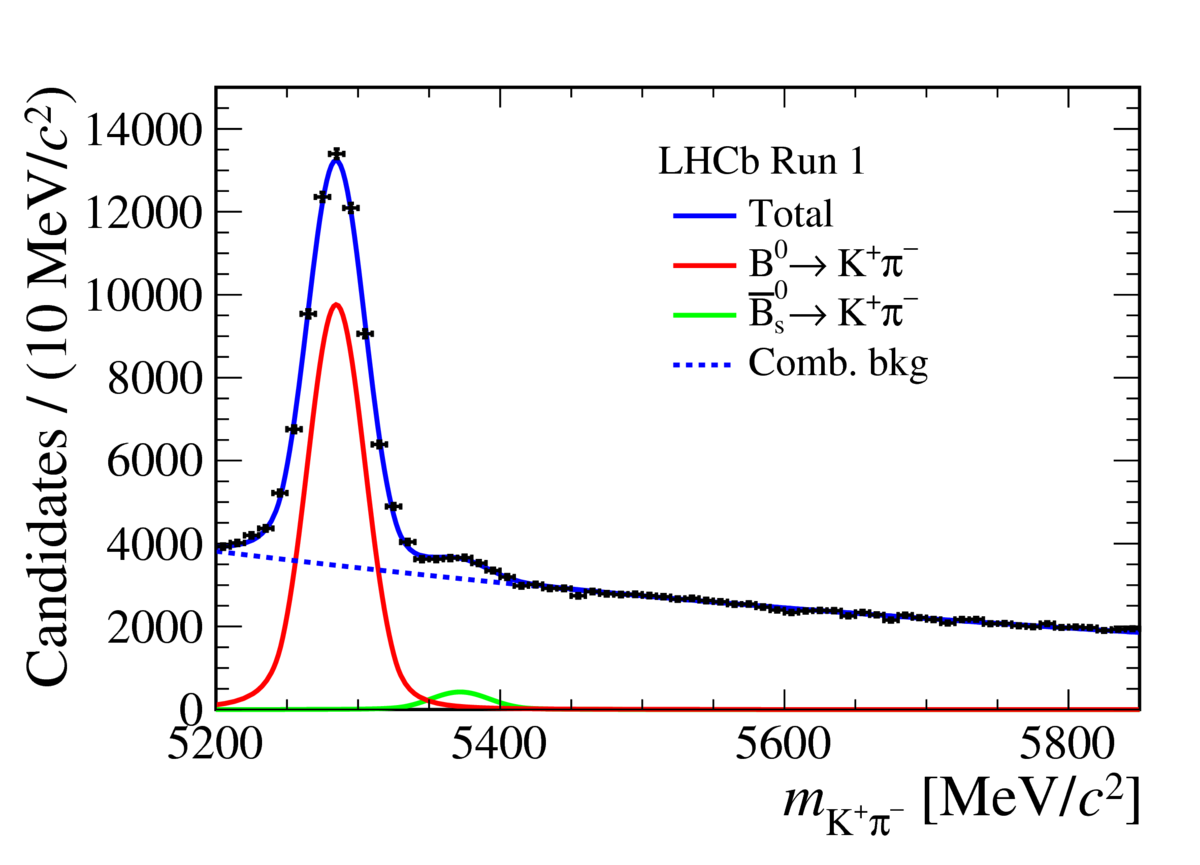
\includegraphics[width= 0.49 \textwidth]{./Figs/BFAnalysis/hidef_Fig9top.png}
     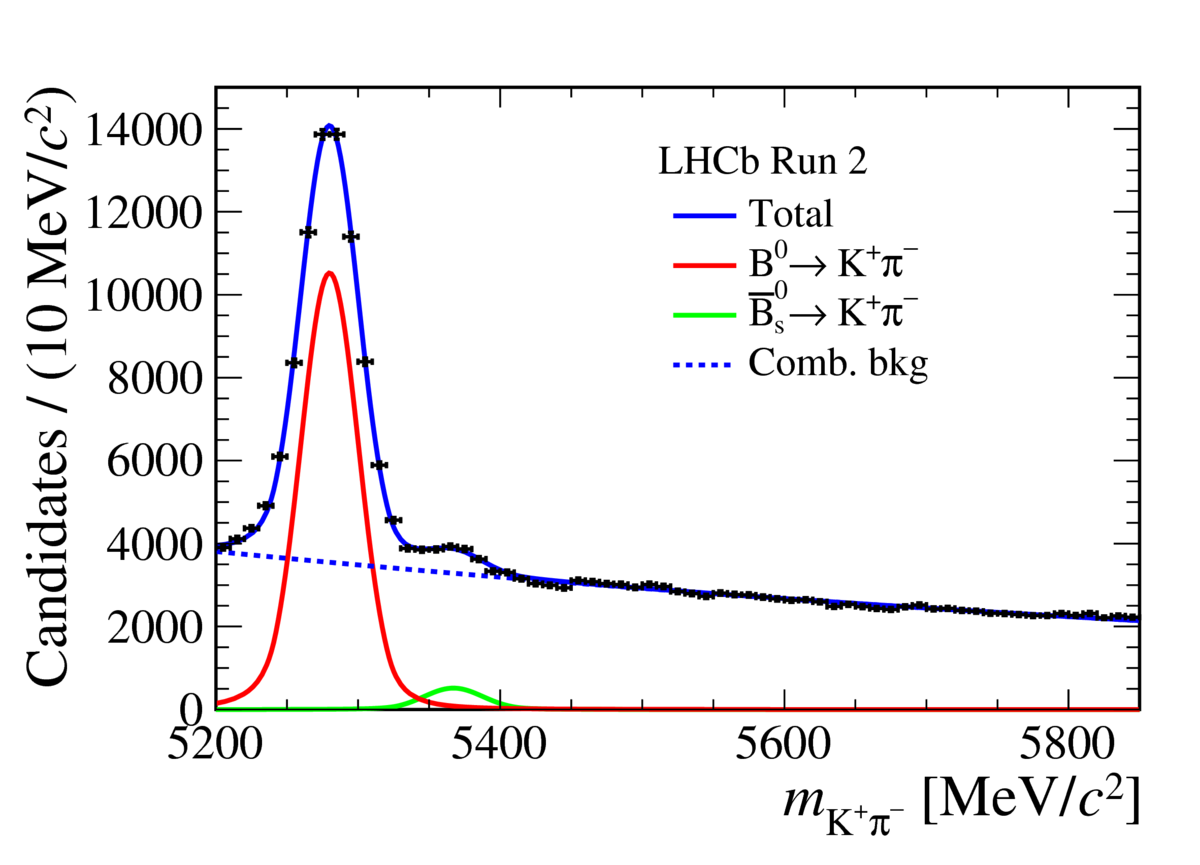
\includegraphics[width= 0.49 \textwidth]{./Figs/BFAnalysis/hidef_Fig9bot.png}
     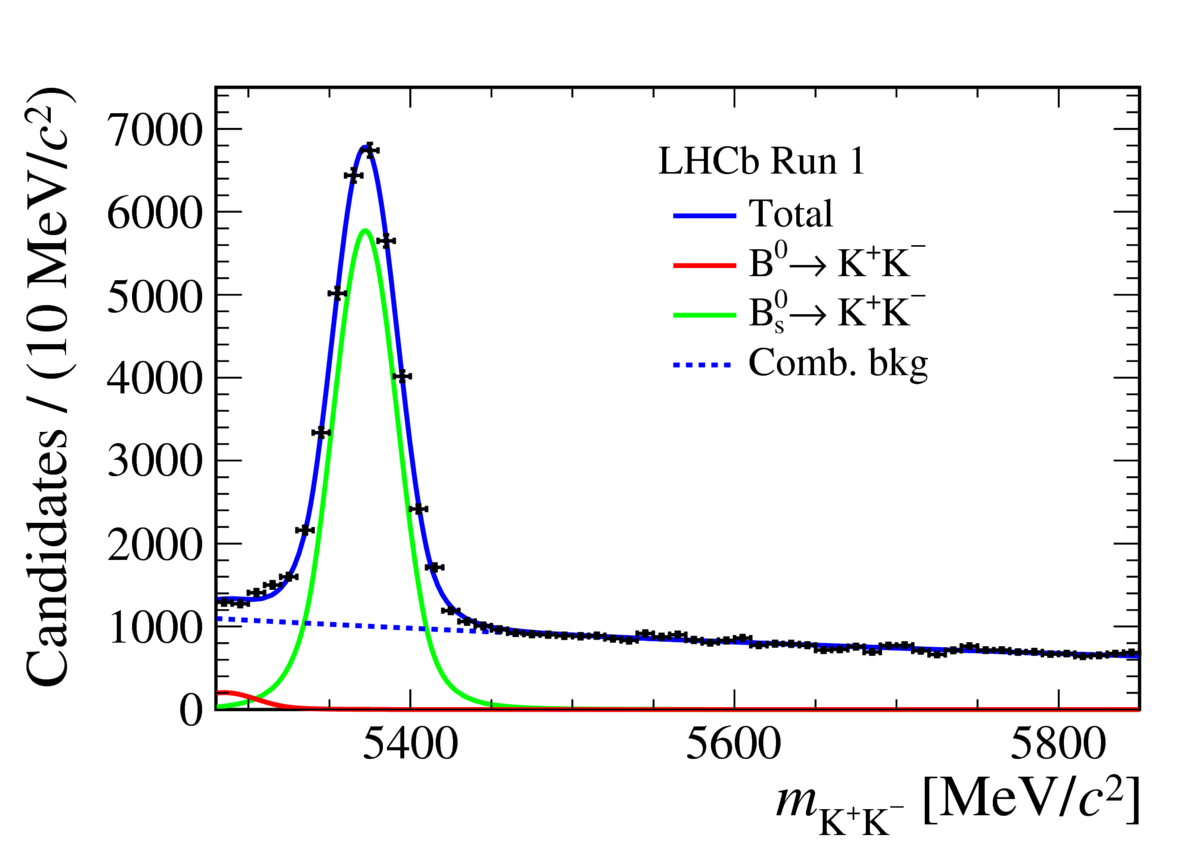
\includegraphics[width= 0.49 \textwidth]{./Figs/BFAnalysis/hidef_Fig10top.png}
     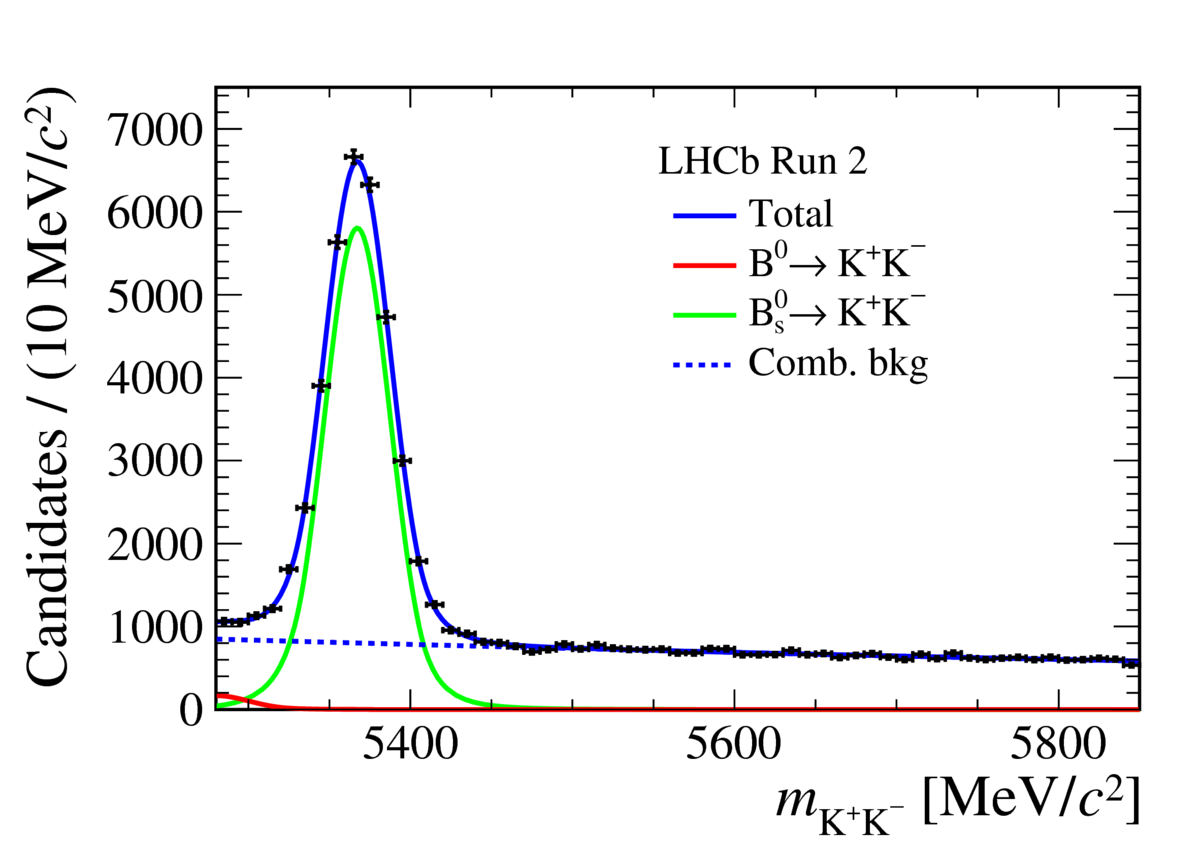
\includegraphics[width= 0.49 \textwidth]{./Figs/BFAnalysis/hidef_Fig10bot.png}
     \caption{Maximum likelihood fits to \bdkpi (top) and \bskk (bottom) for Run~1 and Run~2 data to measure \bd and \bs masses.}
     \label{fig:means}
\end{figure}

\begin{figure}[tbp]
    \centering
     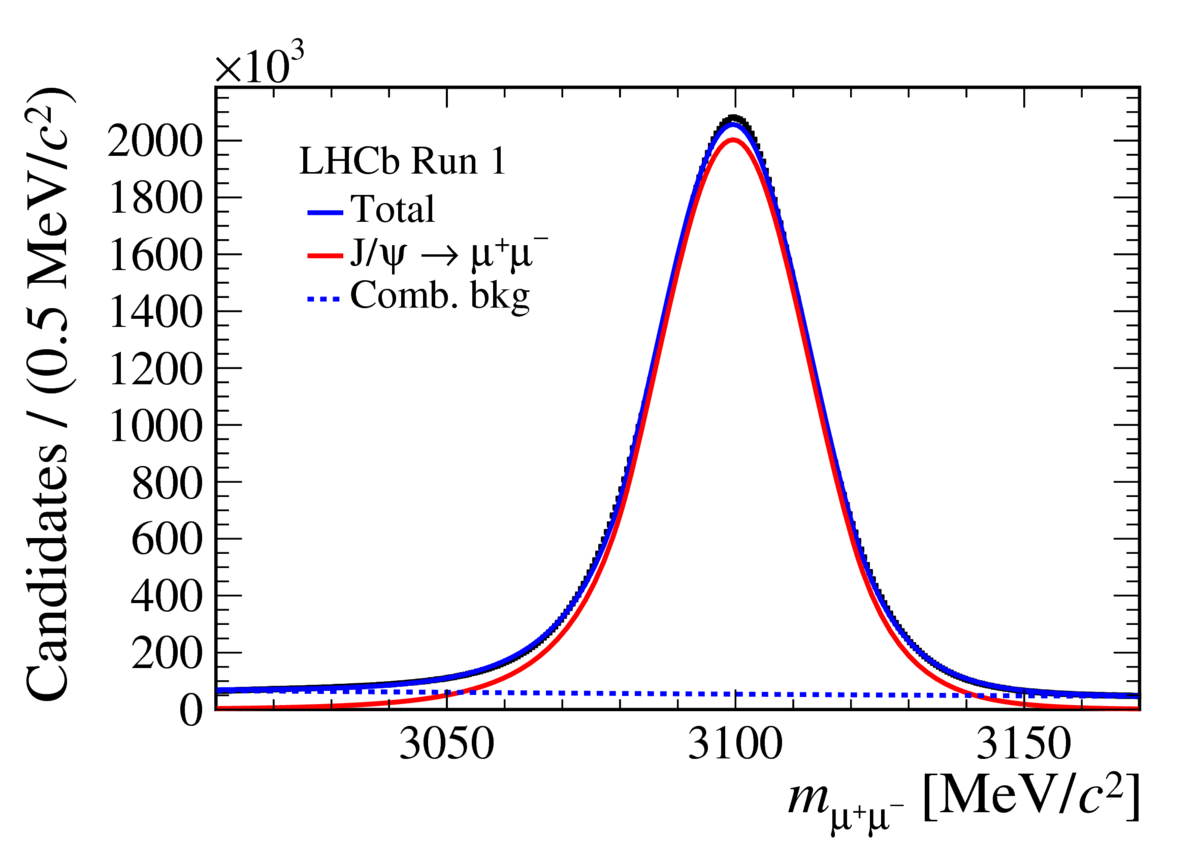
\includegraphics[width= 0.49 \textwidth]{./Figs/BFAnalysis/hidef_Fig11top.png}
     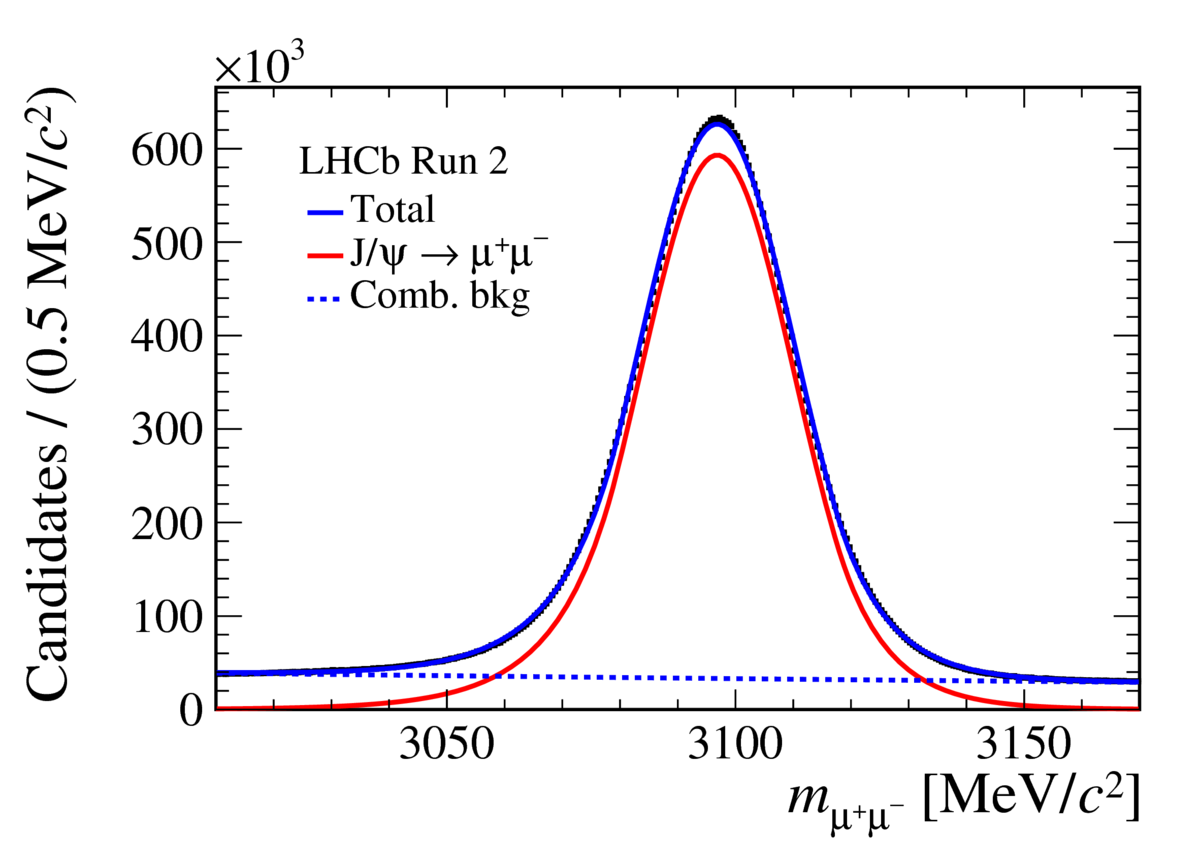
\includegraphics[width= 0.49 \textwidth]{./Figs/BFAnalysis/hidef_Fig11bot.png}
     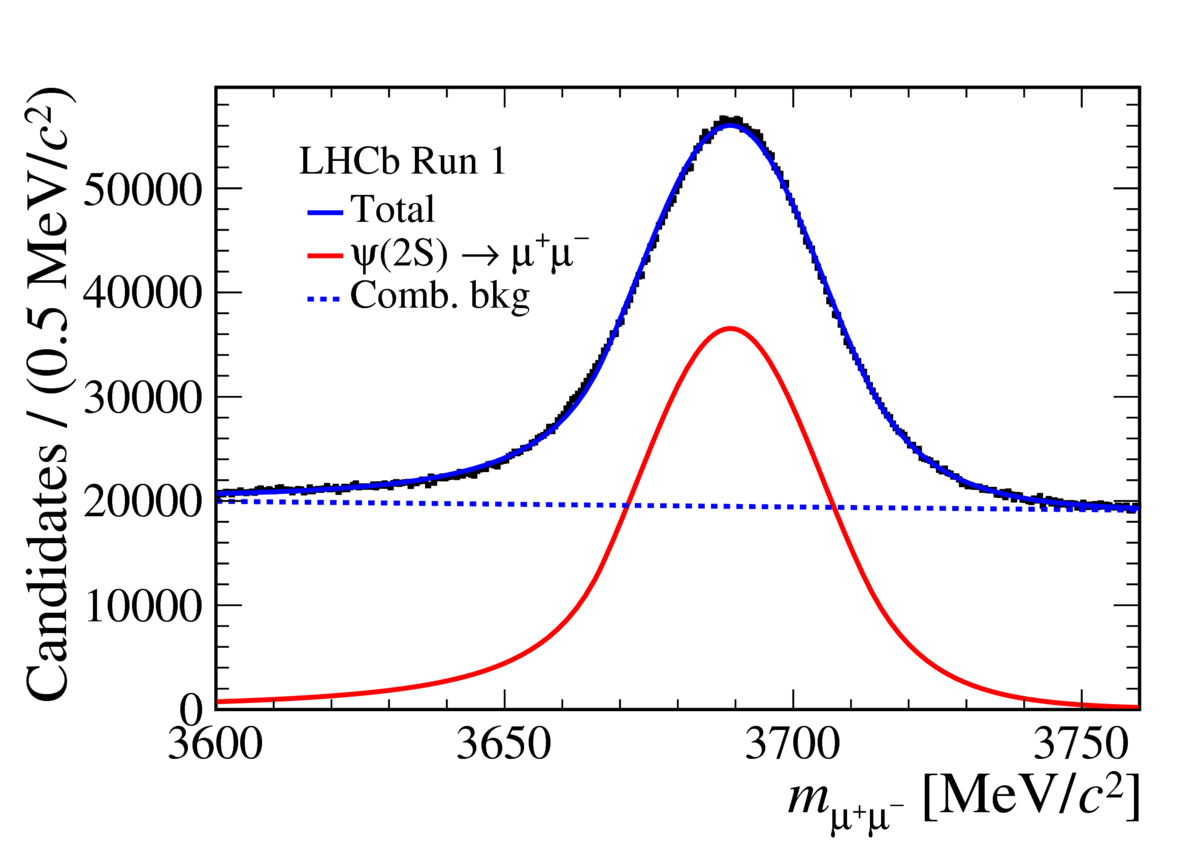
\includegraphics[width= 0.49 \textwidth]{./Figs/BFAnalysis/hidef_Fig12top.png}
     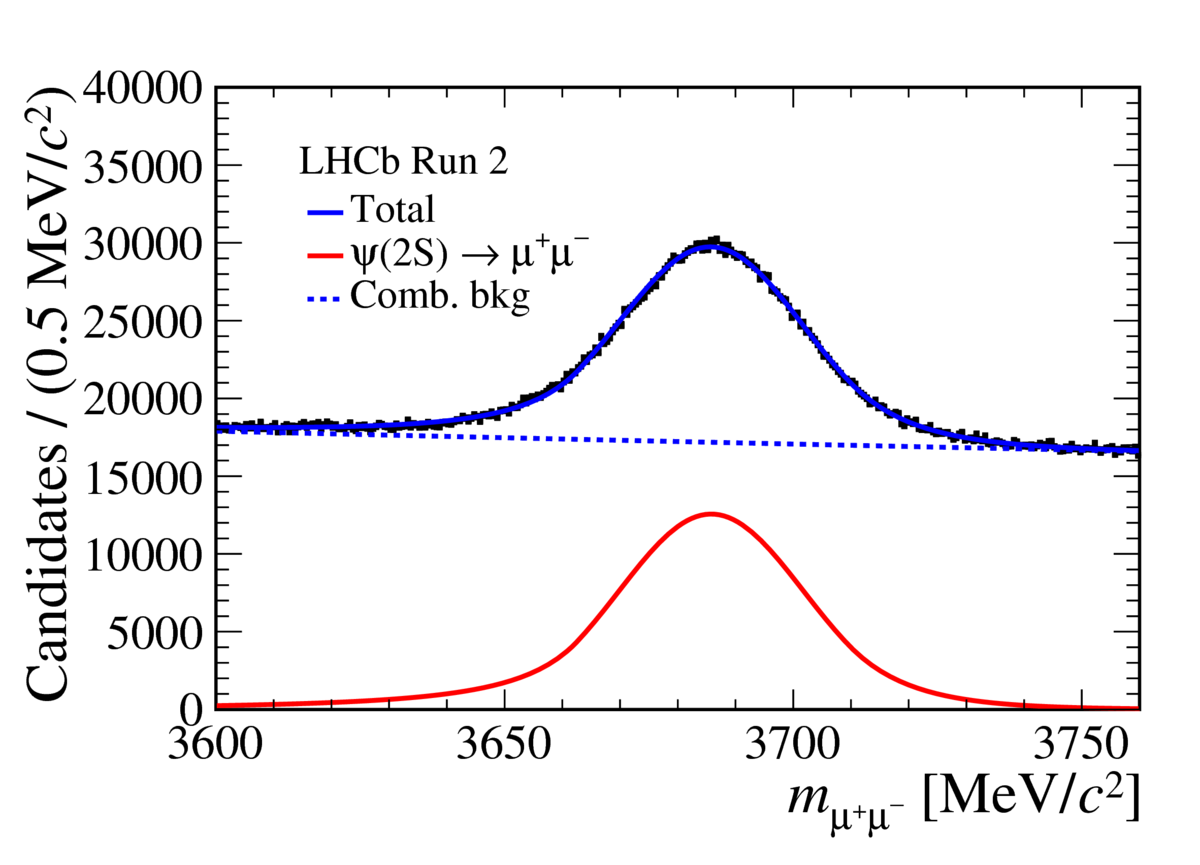
\includegraphics[width= 0.49 \textwidth]{./Figs/BFAnalysis/hidef_Fig12bot.png}
     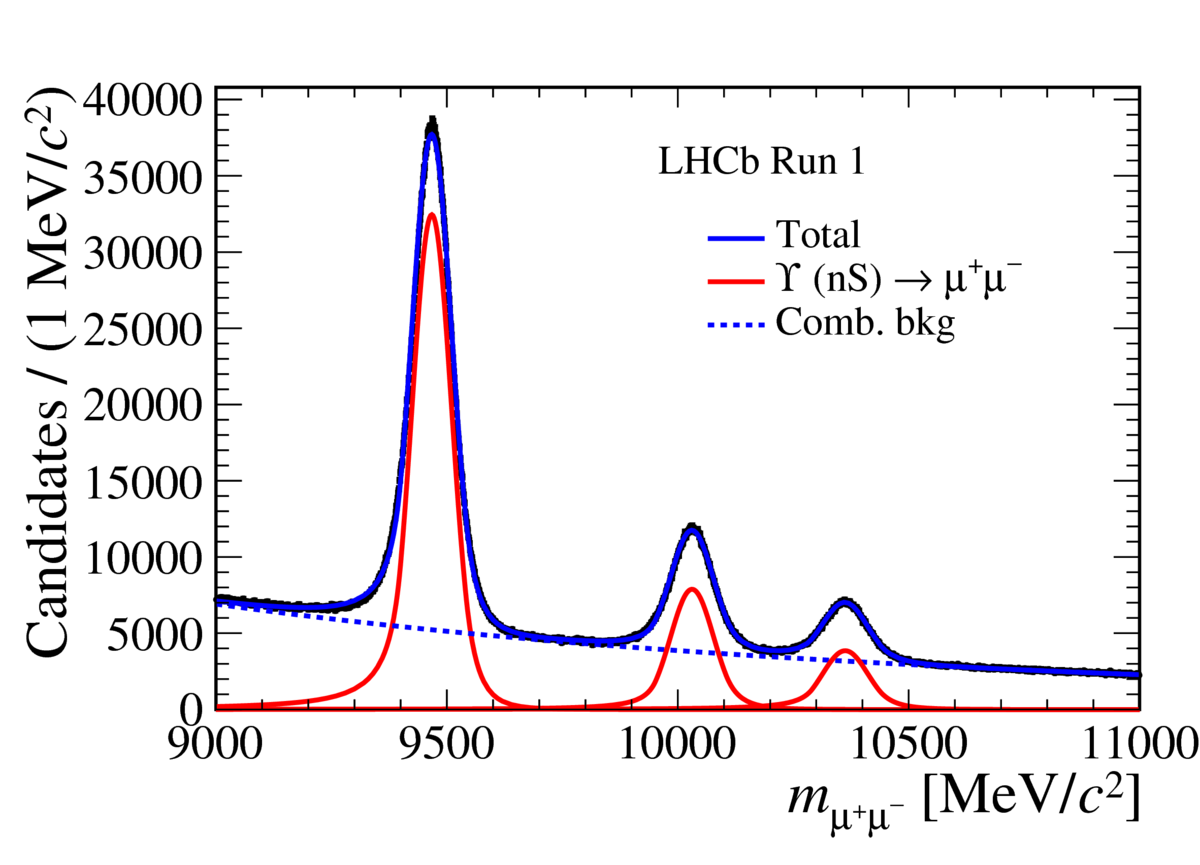
\includegraphics[width= 0.49 \textwidth]{./Figs/BFAnalysis/hidef_Fig13top.png}
     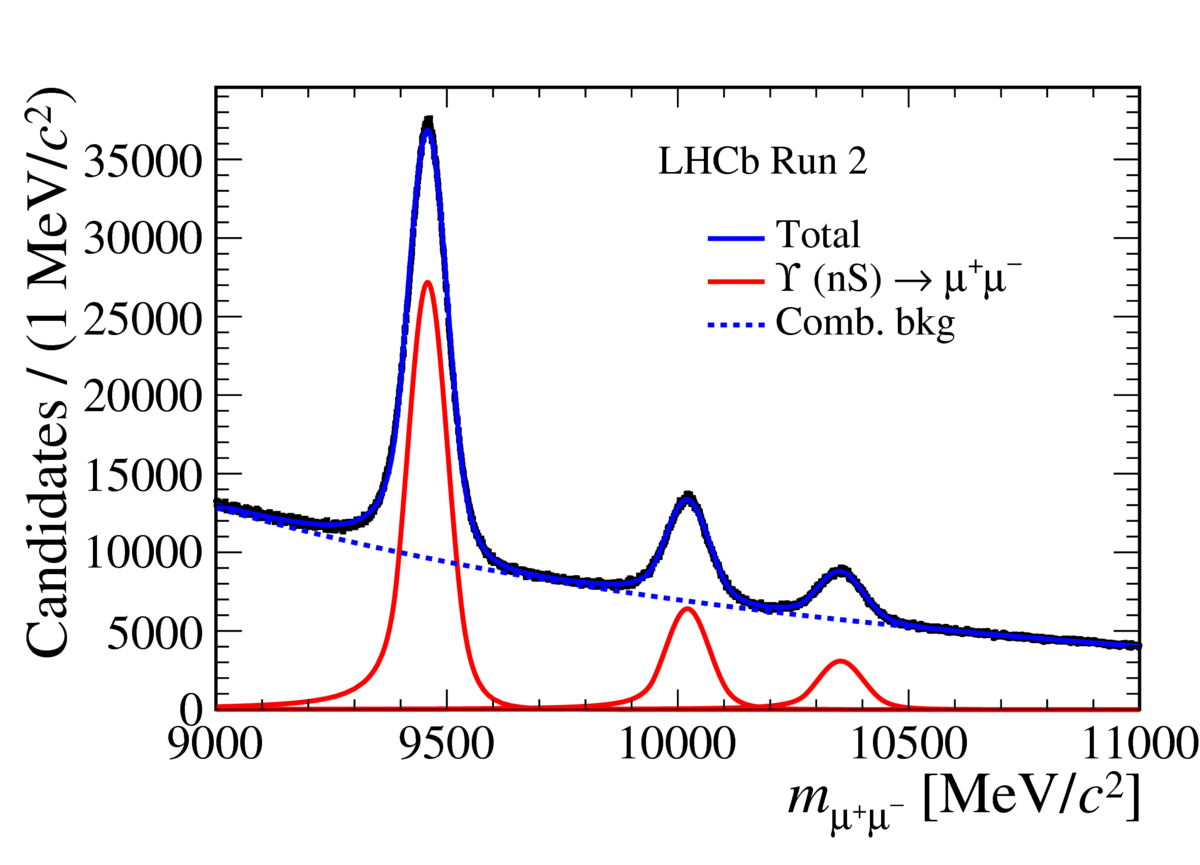
\includegraphics[width= 0.49 \textwidth]{./Figs/BFAnalysis/hidef_Fig13bot.png}
     \caption{Maximum likelihood fit to the mass spectrum of \jpsi (top), $\Psi (2S)$ (centre) and $\Upsilon(1, 2, 3S)$ (bottom) decaying into two muons in Run~1 and Run~2 data.}
     \label{fig:quarkonia}
\end{figure}

\begin{figure}[tbp]
    \centering
     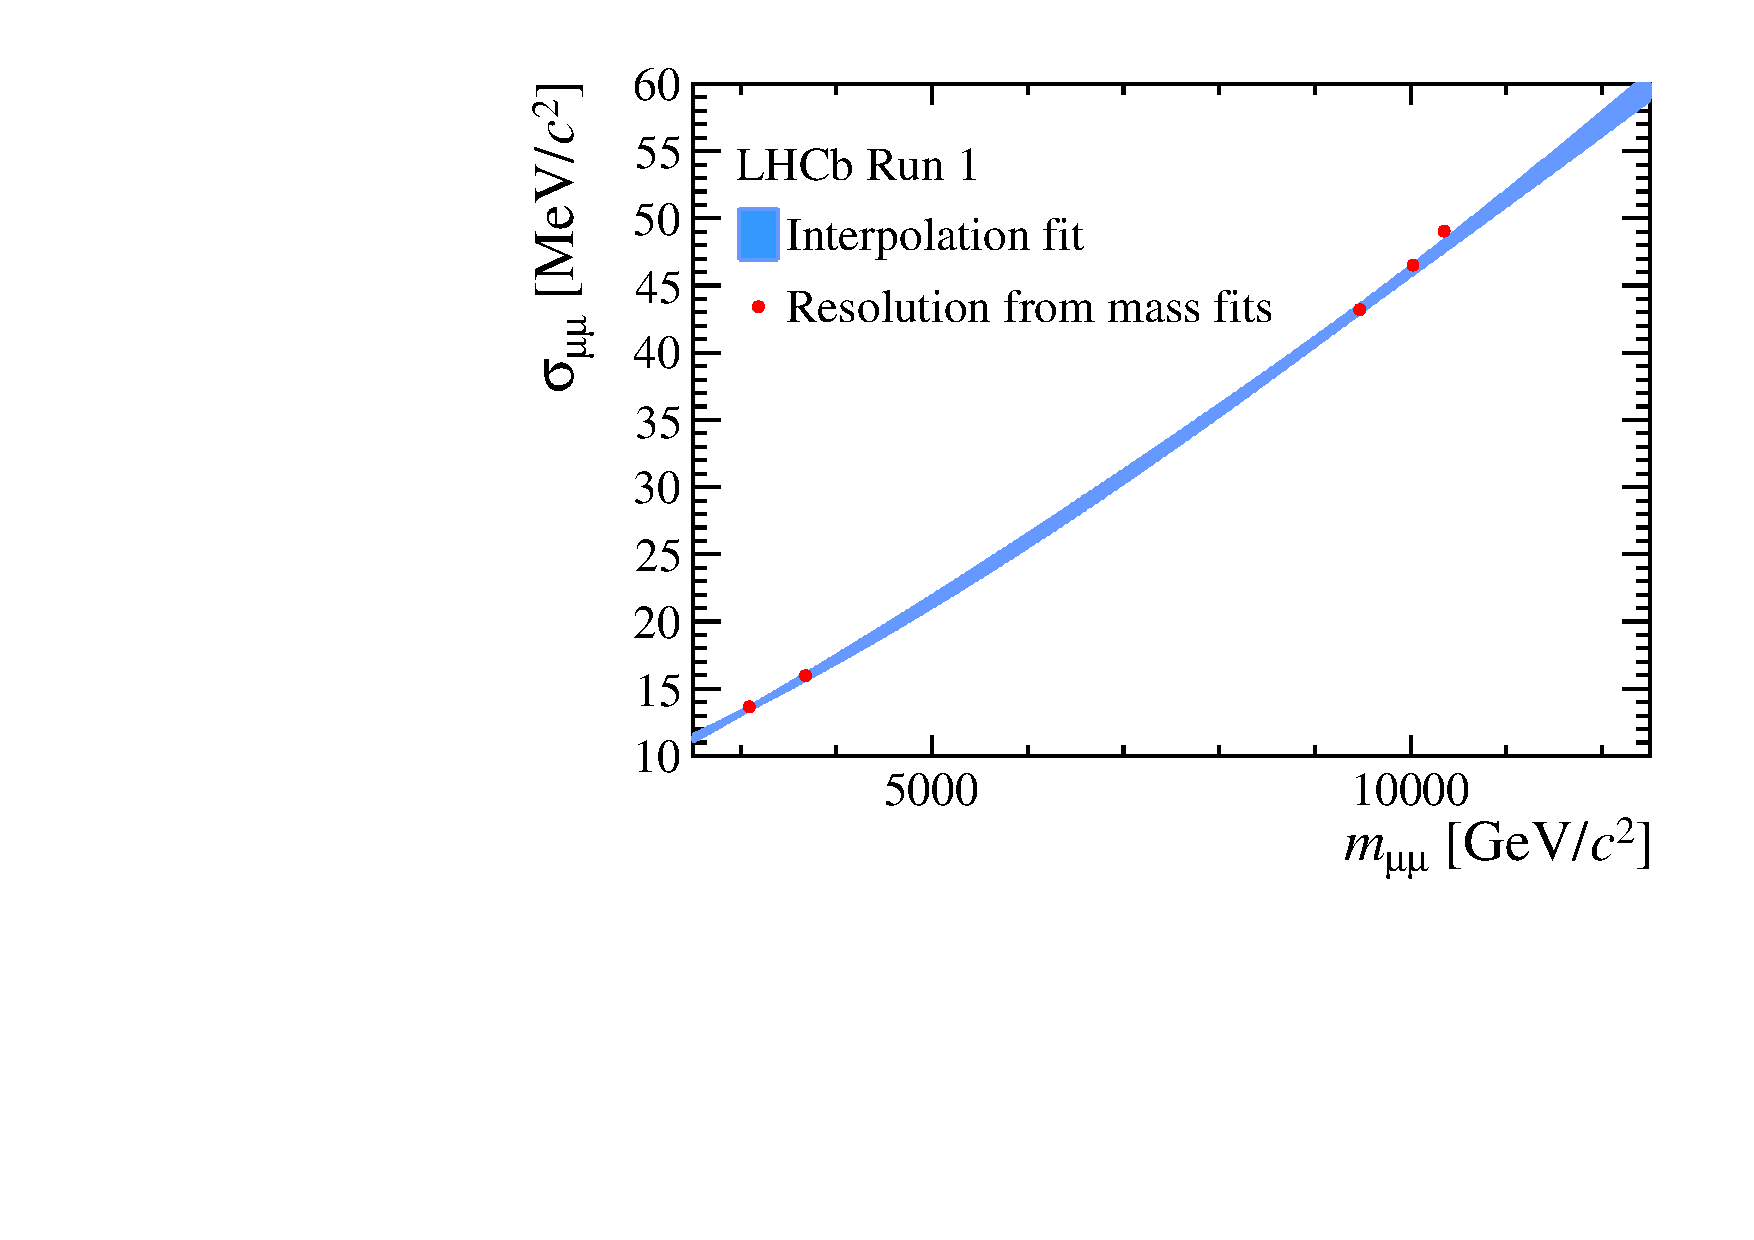
\includegraphics[width= 0.49 \textwidth]{./Figs/BFAnalysis/Run1_res.pdf}
     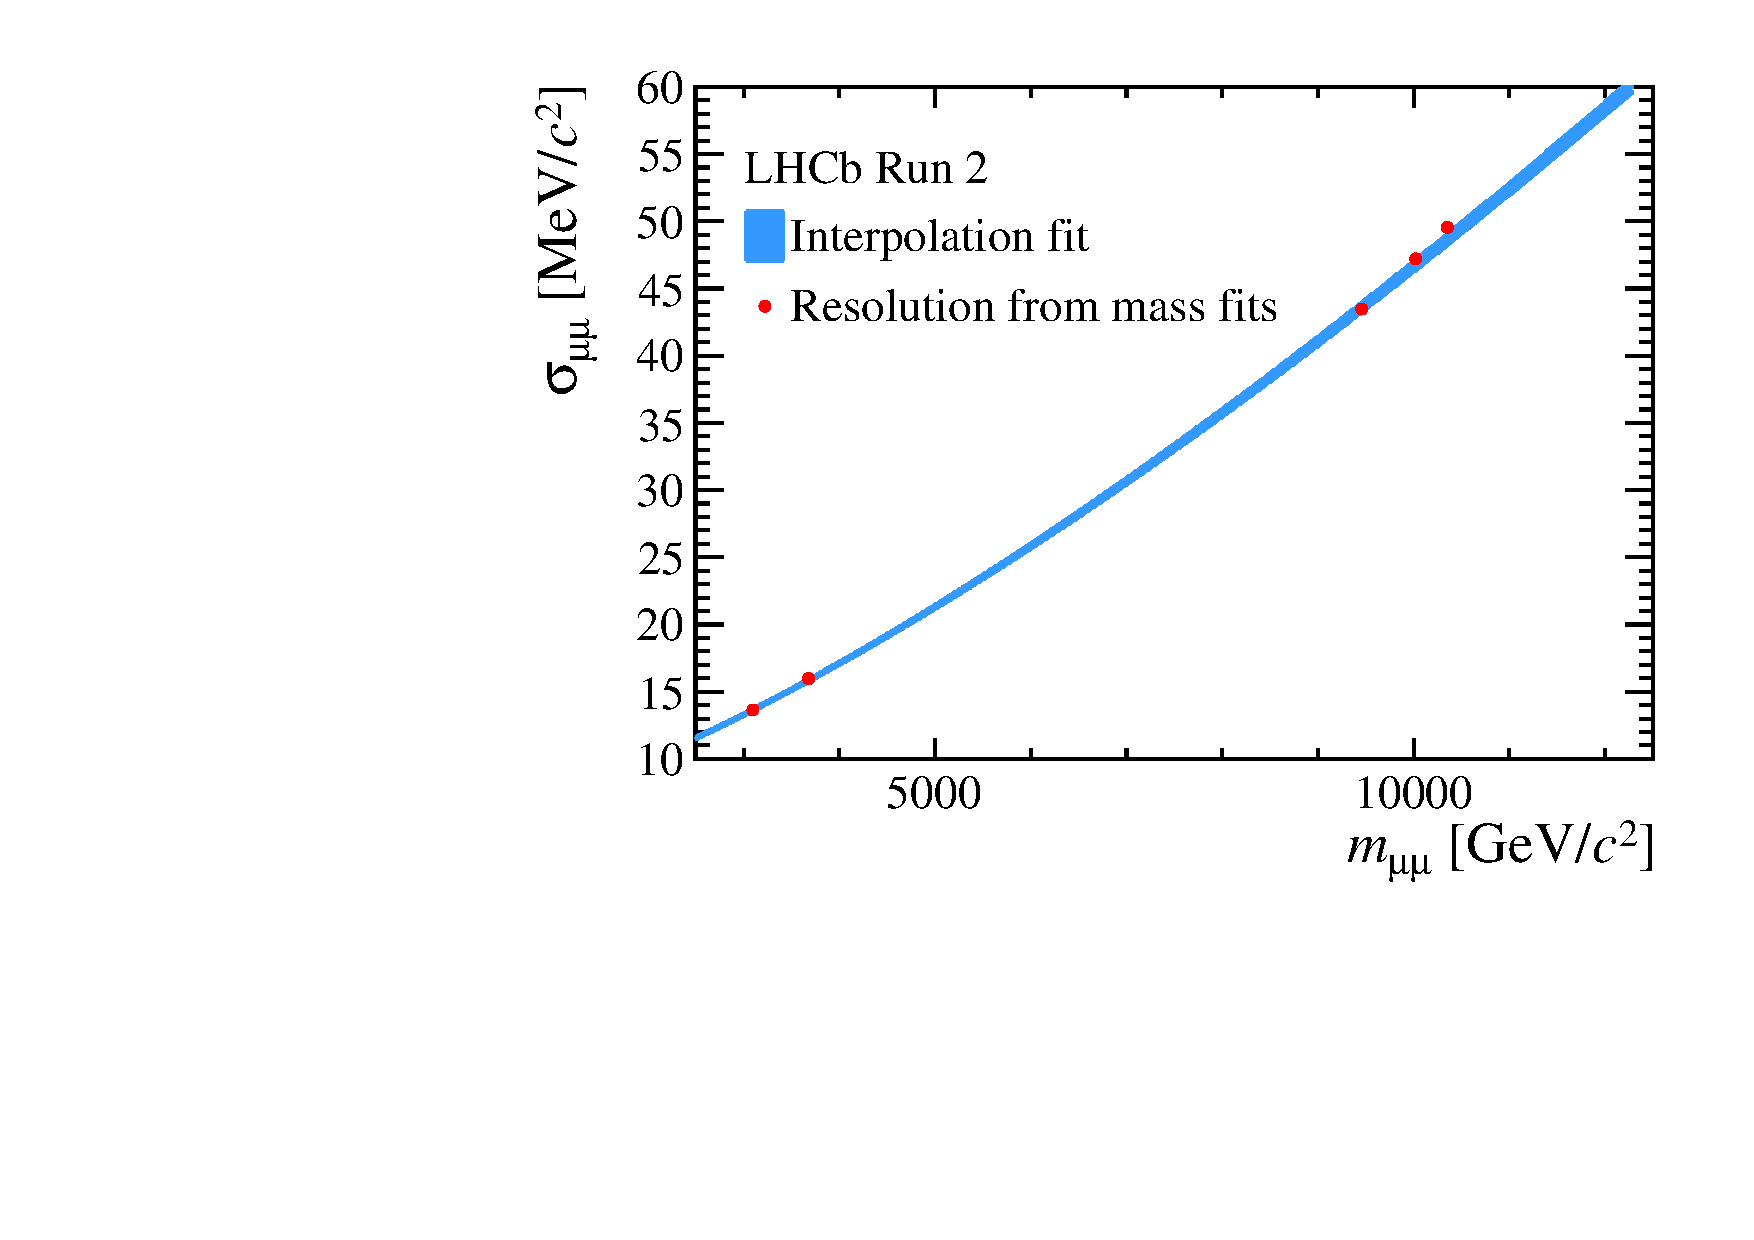
\includegraphics[width= 0.49 \textwidth]{./Figs/BFAnalysis/Run2_res.pdf}
     \caption{Power law fit to the resolution of quarkonia resonances to determine mass resolution for \bdmumu and \bsmumu decays on Run~1 and Run~2 data.}
     \label{fig:interp}
\end{figure}

\subsection{BDT \pdfs}
\label{sec:ADGBDTcorrections}                                                                                                                

%The fraction of \bmumu decays in each BDT bin is meeded to measure the branching fraction therefore the BDT \pdf needs to be evaluated. 
The global BDT distribution for \bmumu decays is expected to be uniform between 0 and 1 as designed by the flattening procedure described in Section~\ref{BDTS}. The fraction of \bmumu decays in a BDT bin should be proportional to the bin width. However, the global BDT was trained and flattened using simulated decays, therefore to avoid differences between simulated decays and data affecting the expected fraction of \bmumu decays in each BDT bin, the BDT \pdf is evaluated from \bdkpi decays in data. This process is known as the BDT calibration.
The global BDT is designed to use only kinematic and geometric information to classify candidates and includes no PID information. Therefore the BDT distributions of \bdkpi decays will be the same to a good approximation as \bmumu decays since they are kinematically very similar. %\bdkpi decays are used to calibrate the BDT response because it is the most abundant \bhh decay. 

The number of \bdkpi decays is extracted from data by fitting the mass distribution of \bdkpi candidates in each BDT bin for Run~1 and Run~2 data. The \bdkpi candidates must pass the standard \bhh selection outlined in Section~\ref{sec:BFsel} and are separated from other \bhh modes using the DLL$_{K\pi}$ variable. %To reduce the difference in the trigger efficiency between \bdkip and \bmumu decays, \bdkpi candidates are required to be TIS at L0 and Hlt1, but TOS at Hlt2, to ensure enough statistics.

The particle identification and trigger efficiencies are different for \bdkpi and \bmumu decays. Therefore, the \bdkpi yields in each BDT bin are corrected for the different efficiencies. %this. %for using by the different trigger and particle identification efficiencies. 
The same calibration is used for \bdmumu and \bsmumu decays.
The calibration is performed for each year separately then combined to give the Run 1 and Run 2 fractions per BDT bin. Figure~\ref{fig:BDTpdfs} shows the BDT distribution for \bmumu decays calibrated with \bdkpi data for Run 1 and Run 2. 
The systematic uncertainties on the BDT calibration arise from the mass range used in the fit, the choice of the fit model and particle identification requirements and the trigger and particle identification efficiency corrections.
\begin{figure}[tbp]
    \centering
   \begin{subfigure}[b]{0.48\textwidth}
        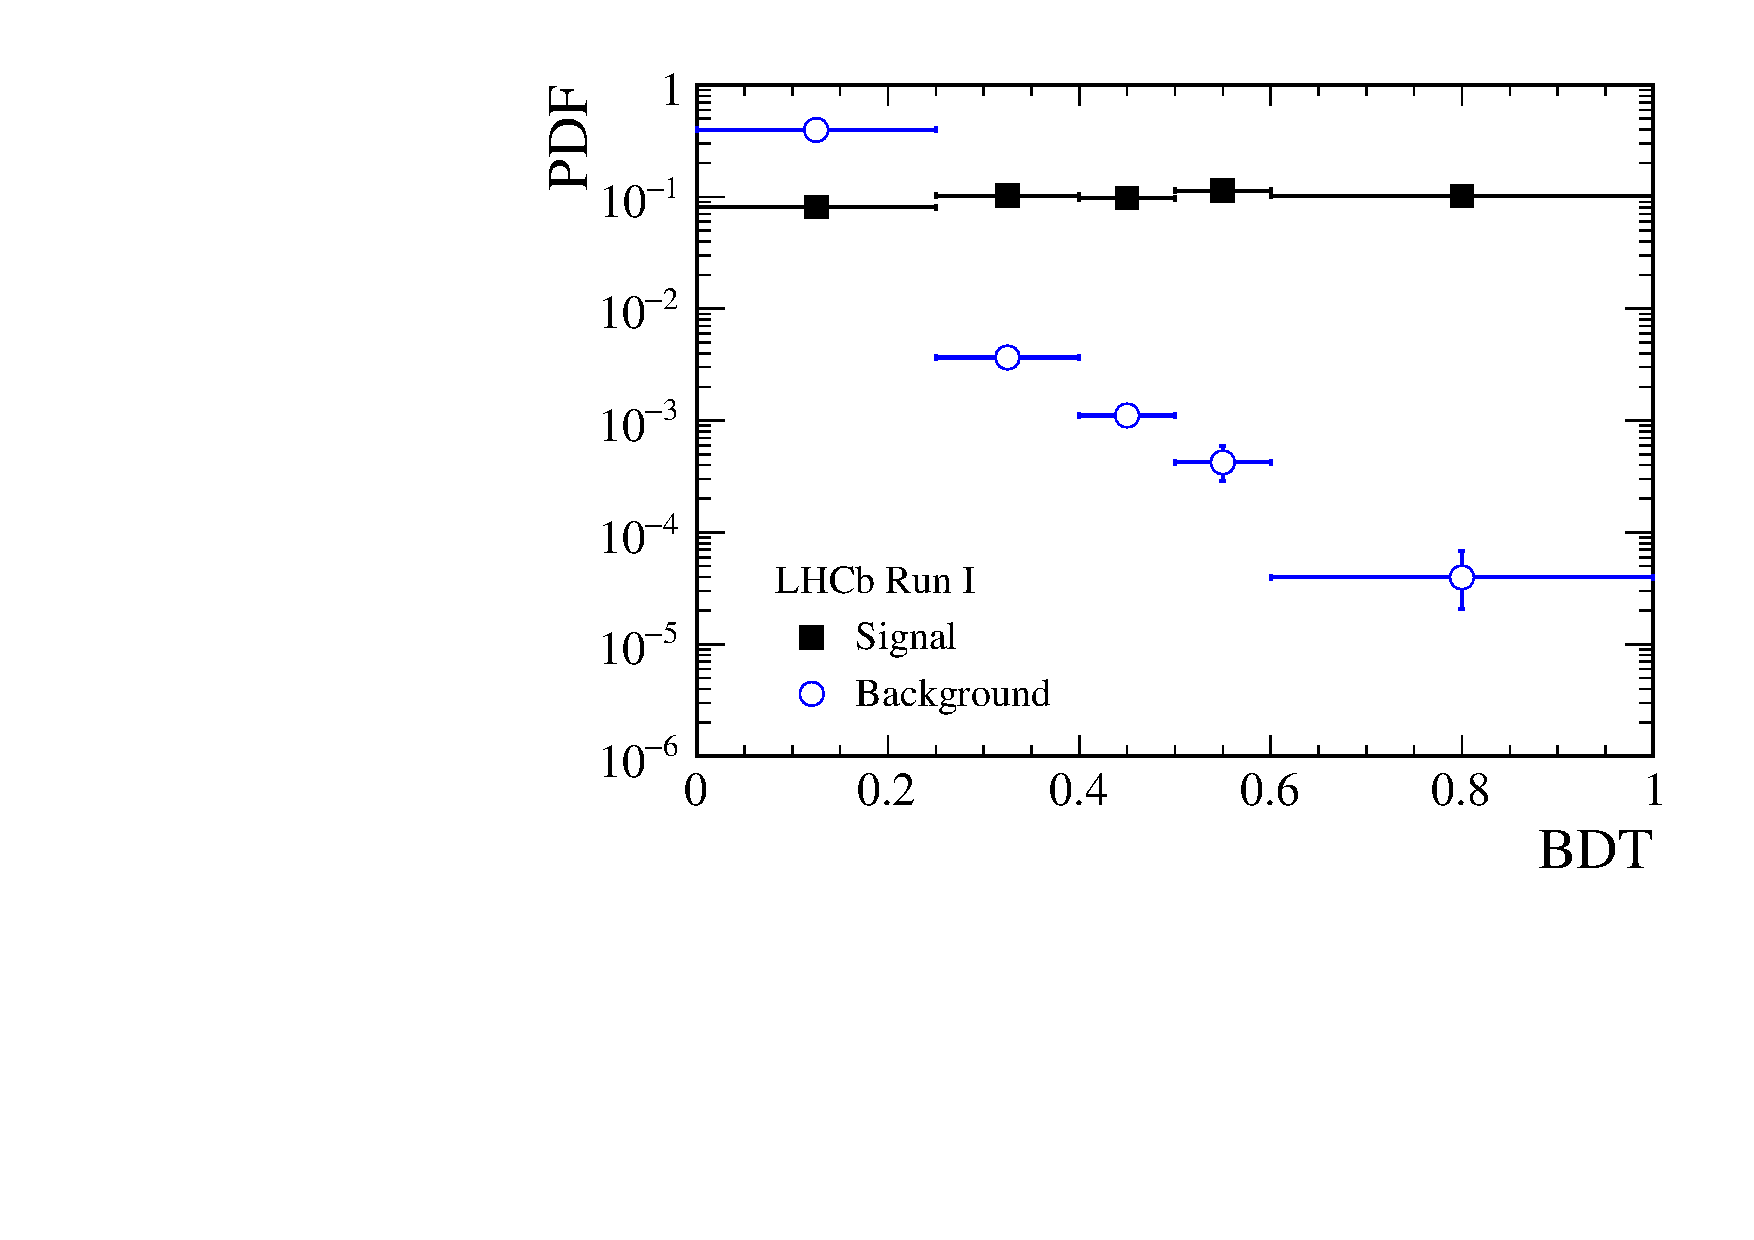
\includegraphics[width= \textwidth]{./Figs/BFAnalysis/C_macros/BDT_calibration_Run1.pdf}
        %\caption{ }
       % \label{fig:BDTSsig}
    \end{subfigure}
   % ~ %add desired spacing between images, e. g. ~, \quad, \qquad, \hfill etc. 
      %(or a blank line to force the subfigure onto a new line)
    \begin{subfigure}[b]{0.48\textwidth}
       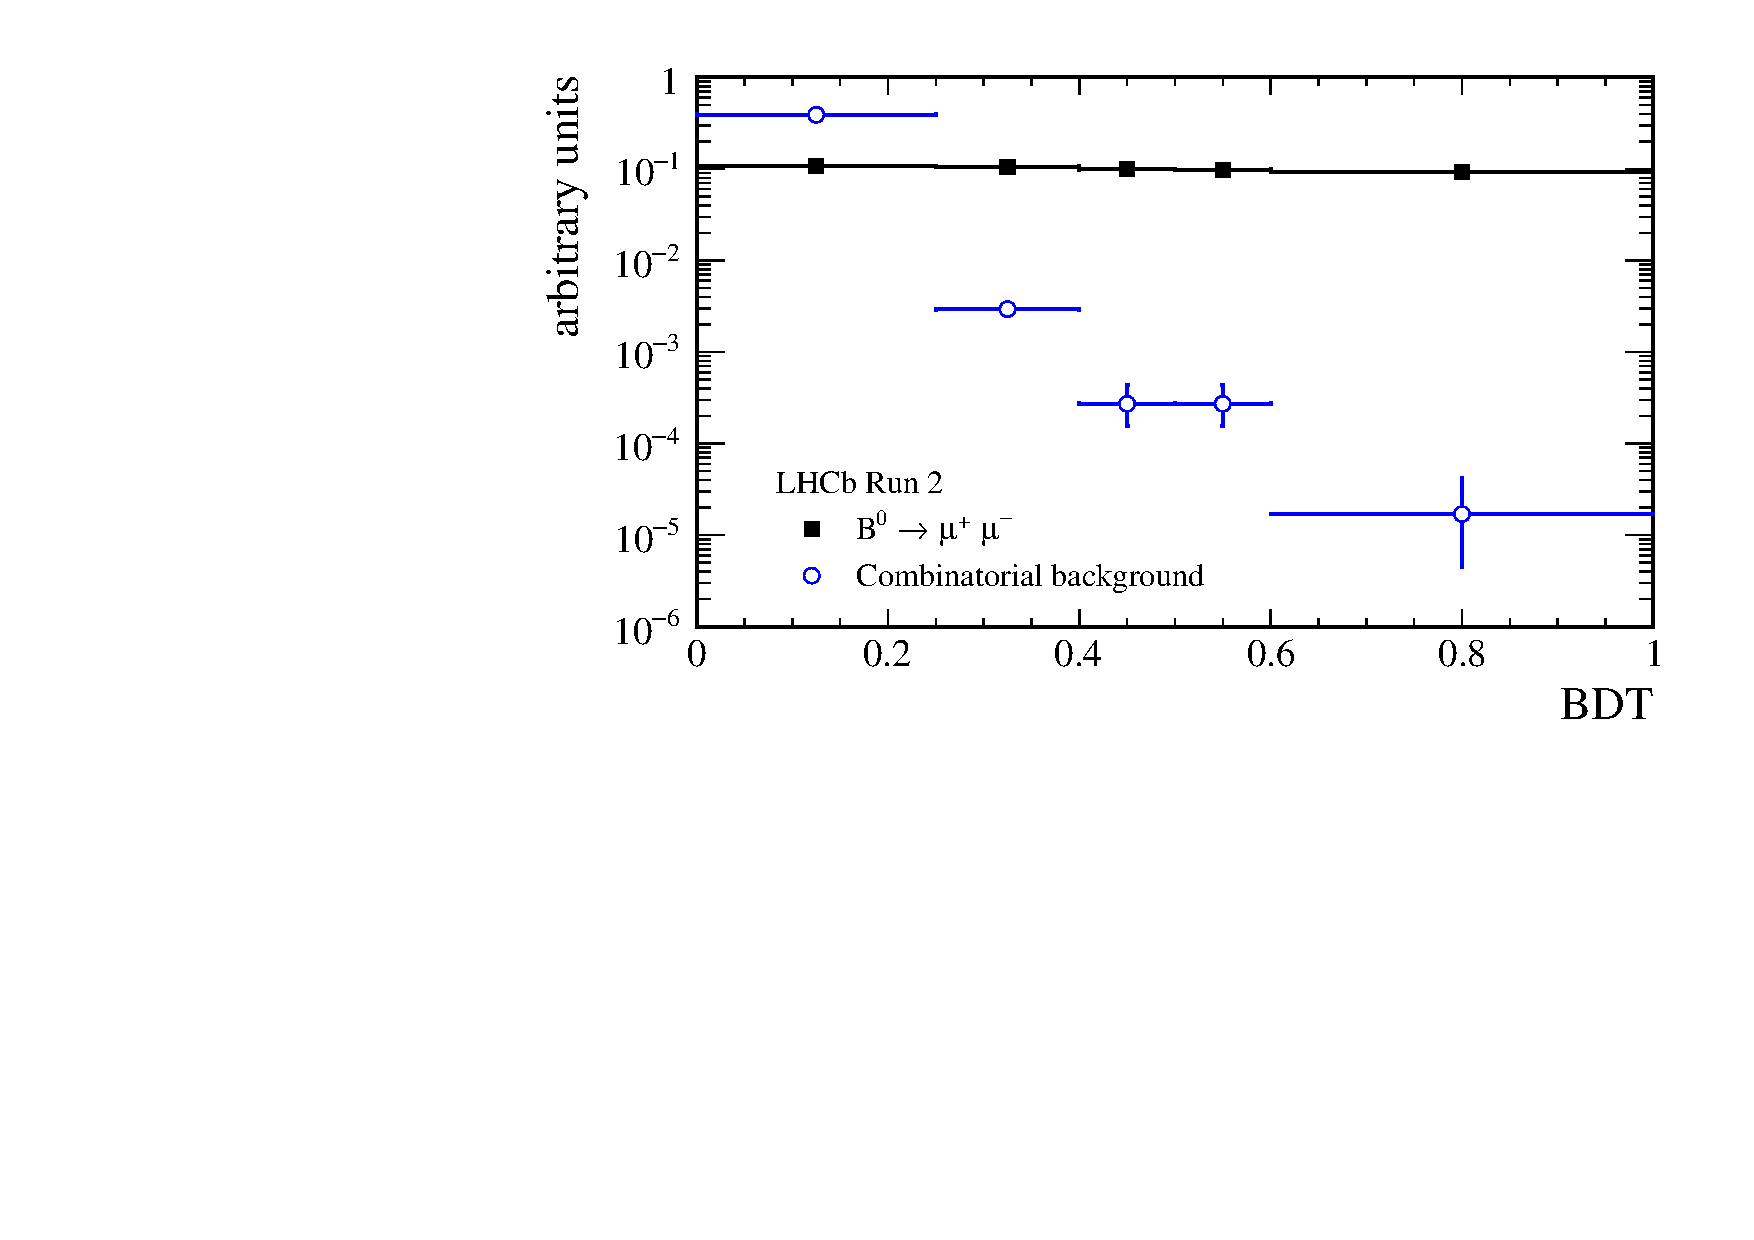
\includegraphics[width=\textwidth]{./Figs/BFAnalysis/C_macros/BDT_calibration_Run2.pdf}
      %  \caption{ }
     %   \label{fig:BDTSbkg}
   \end{subfigure}
    \caption{\bmumu BDT \pdfs (black squares) for Run 1 and Run 2 data calibrated using \bdkpi decays and the combinatorial background decays (blue circles) for \bmumu candidates in data with a dimuon mass above 5477 \mevcc. The uncertainties on the signal fractions are included on the plots but are too small to be visible. }
    \label{fig:BDTpdfs}
\end{figure}


%\subsection{Decay time dependence}% of the \bsmumu BDT \pdf}
%\label{sec:ADGBDTcorrections}
Although the BDT is calibrated, the dependence of the BDT response on the \bsd candidate decay time must also be considered. 
The response of the global BDT for \bmumu decays is correlated with their decay time due to the use of the \bs IP and \chiIP and isolation criteria as inputs to the BDT. This correlation will lead to slightly incorrect estimations of the \bsmumu BDT \pdf. In the SM the \bsmumu effective lifetime, \tmumu, is equal to the lifetime of the heavy \bs mass eigenstate, \tH. However in reality \tmumu could be somewhere in between the lifetimes of the heavy and light mass eigenstates. As described in Chapter~\ref{sec:theory_chptr} the \bsmumu effective lifetime is related to the parameter \ADG, where \ADG = +1 for \tmumu = \tH and \ADG = $-1$ for \tmumu = \tL, where \tL is the lifetime of the light \bsmumu mass eigenstate.

The simulated decays used to train and flatten the global BDT use as the \bsmumu lifetime the mean of the measured \tH and \tL values at the time of the simulation production~\cite{Olive:2016xmw}. Therefore, the lifetime used is different between simulation versions. Since the BDT output is correlated with the lifetime, the fraction of \bsmumu decays in each BDT bin will depend on the lifetime used in the simulation. Numerical correction factors are computed for each year to scale the fraction of \bsmumu decays in each BDT bin for the situations where \ADG = $-1$, 0 or +1, so that the dependence on \ADG of the measured branching fractions can be evaluated.

No corrections are needed for \bdmumu because the difference in lifetime of the heavy and light \bd mass eigenstates is negligible and the need for correction cancels out with the BDT calibration that uses the \bd decay \bdkpi. 

%{\it I have some questions about this part, how are these corrections actually used since the BDT is flattened for Run 1 with 2011 and for Run 2 with 2015 MC.How is the callibration ok since it uses the B0 which has the same correlations which is this not taken into accout? Prehaps make this briefer?}

\section{Background mass \pdfs and expected yields}
\label{sec:backgrounds}
The selection described in Chapter~\ref{selection_chapter} is effective at reducing the backgrounds in the data set to a suitable level so that number of the \bmumu decays can be measured. However, some background decays remain in the final data set that cannot be completely removed without drastically reducing the signal efficiency. %The backgrounds present in the data set must be included in the fit to the dimuon invariant mass in order to accurately measure the \bmumu branching fractions. 
The backgrounds present in the final data set originate from:
\begin{itemize}
\item \bhh decays when both hadrons are mis-identified as muons, commonly caused by hadrons decaying semi-leptonically during their flight through the detector after leaving the VELO. This background peaks within the \bd mass window but not the \bs mass window due to the missing energy from the undetected neutrino;
\item semi-leptonic decays where one hadron is mis-identified as a muon that include
\begin{itemize}
\item \bdpimunu and \bsKmunu decays where the final state hadrons are mis-identified as muons. The majority of these backgrounds falls below the \bd mass window in the left mass sideband; and
\item \lambdab decays when the proton is mis-identified as a muon. This background produces a small number of decays with masses within the \bs and \bd mass windows and at in the left mass sideband;
\end{itemize}
\item decays which contain two muons that form a good vertex that include
\begin{itemize}
\item \bpimumu decays where the pion is not detected. The missing hadron means that these backgrounds fall well below the \bd mass window; and
\item \bcjpsimunu decays where \jpsimumu. The large mass of the $B^{+}_{c}$ causes this background to cover the full mass range 4900 - 6000 \mevcc; and
\end{itemize}
\item combinatorial background formed by the random combination of any two muons in the event, this background is distributed across the full mass range.
\end{itemize}

The backgrounds present in the data set must be included in the fit to the dimuon invariant mass in order to accurately measure the \bmumu branching fractions.
Therefore, the mass \pdfs and expected yields of each background must be evaluated. The following sections summarise the information used for each background source in the \BF fit and Figure~\ref{fig:BFbkgnds} shows the mass distributions of the background sources for the expected number of candidates with BDT values of BDT~$> 0.5$.

\begin{figure}[tbp]
    \centering
     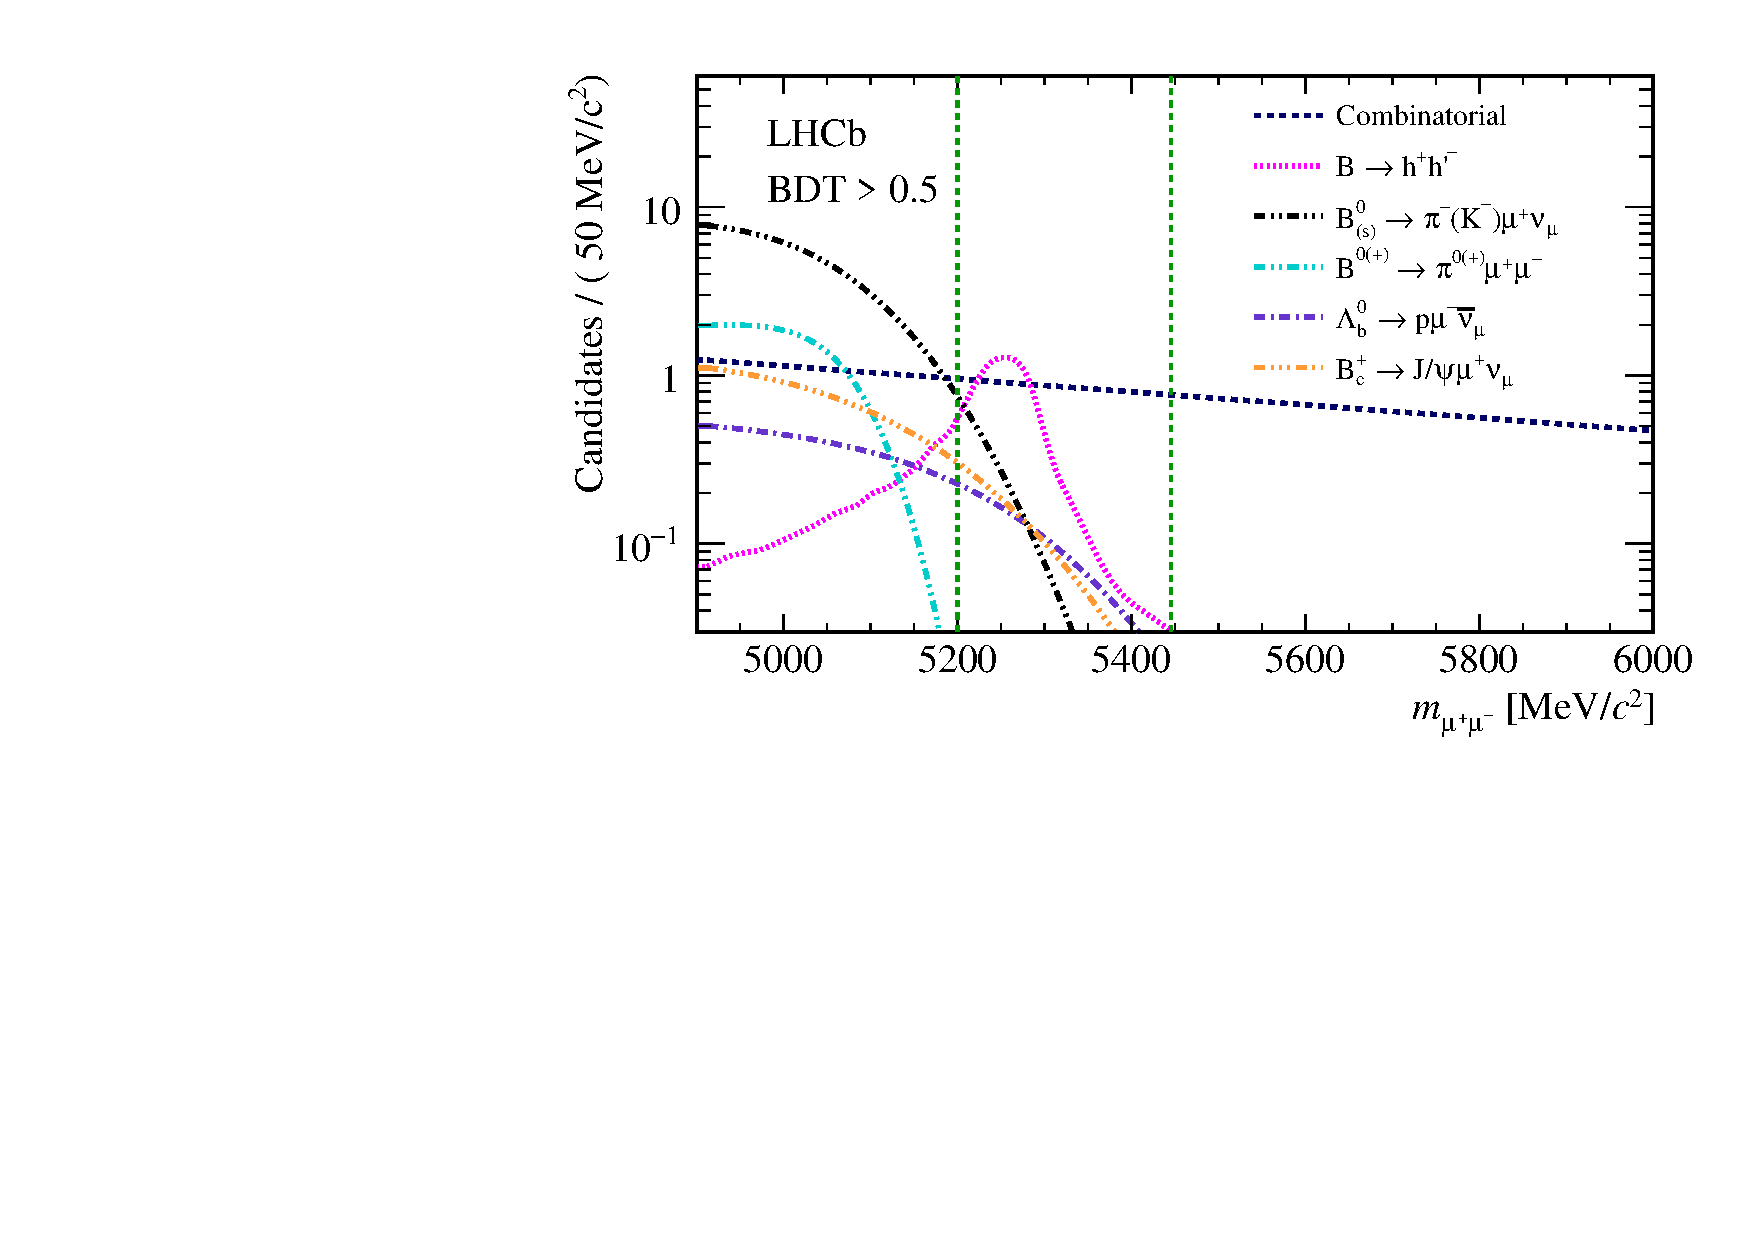
\includegraphics[width= 0.9 \textwidth]{./Figs/BFAnalysis/Fig4.pdf}
     \caption{Mass distributions for \bmumu backgrounds with global BDT values of BDT~$>$~0.5. The backgrounds shown are from \bhh, \bdpimunu, \bsKmunu, \lambdab, \bpimumu, \bcjpsimunu and combinatorial background. The green dashed lines show the \bmumu mass window defined at the start of the chapter. }
     \label{fig:BFbkgnds}
\end{figure}
%To measure the number of \bsmumu decays these backgrounds must be modelled in the invariant mass fit in each BDT bin, therefore the mass \pdfs and fraction of events present in each BDT bin must be determined.  Backgrounds that fall below the \bd and \bs mass windows still need to be accruatly modelled so that the number of combinatorial background decays that cover the full mass range can be accuratley described/measured. The proceedure is slightly different for \bhh decays compared to semi-leptonic decays.
%In the fit to the dimuon invariant mass the combinatorial background is modelled by an exponential function. The combinatorial background yield is not constrained in the fit and the slope is required to have the same value across all BDT bins for each data set. These parameters are determined from a simultaneous fit to candidates in data in BDT bins for the mass ranges [4900, ($m_{B^{0}} - 60$)] \mevcc and [($m_{B^{0}_{0}$ + 60, 6000] \mevcc, where the mass shapes and yields of the remaining backgrounds are constrained as described in the following sections.
%The mass \pdfs and yields of the background from \bhh and semi-leptonic decays are constrained in the fit around the expected values. The backgrounds that have lower masses than the \bd and \bs must be accurately modelled in the fit to ensure the combinatorial background yield, that spans the full mass range, is accurate described within the signal mass windows. The approaches for finding the mass \pdfs and expected yields differ for \bhh and semi-leptonic backgrounds, these procedures are described in the following sections.

\subsection[Mis-identified \bhh decays]{Mis-identified \boldmath{\bhh} decays}% mass and BDT \pdfs}
The mass \pdf describing mis-identified \bhh decays is formed of two Crystal Ball functions. The two functions have the same mean but all other parameters can be different and the power-law tails for each function are on opposite sides of the mean value. This combination of functions is called a double Crystal Ball function. The parameter values are evaluated from simulated \bdkpi, \bskk, \bdpipi and \bskpi decays in which the momenta of tracks are smeared to model the hadrons decaying in flight. The parameters are evaluated separately for each \bhh decay and combined using the branching fractions and the particle identification efficiencies for each decay. The mass \pdfs are evaluated separately for Run~1 and Run~2 data and the same \pdf is used for all BDT bins.

The total number of mis-identified \bhh decays expected in Run 1 and Run 2 data, $\mathcal{N}_{B \to hh \to \mu \mu}$, is found using the relationship
\begin{equation}
\mathcal{N}_{B \to hh \to \mu \mu} = \epsilon^{TRIG}_{B^{0}_{(s)} \to \mu \mu} \cdot \frac{\mathcal{N}_{B \to hh}}{\epsilon^{TRIG}_{B \to hh}} \cdot \epsilon_{B \to hh \to \mu\mu}  \\
\label{eq:bhhprediction}
\end{equation}
where ${\mathcal{N}_{B \to hh}$ is the number of TIS \bhh decays in data, $\epsilon^{TRIG}_{B^{0}_{(s)} \to \mu \mu, B \to hh}$ are the \bmumu and \bhh trigger efficiencies and $ \epsilon_{B \to hh \to \mu\mu}$ is the probability that a \bhh decay is mis-identified as \bmumu. 
The number of \bhh decays is calculated from a fit to the mass distribution of \bdkpi candidates identified in data, the number of \bdkpi candidates is translated into the total number of \bhh by scaling the \bdkpi yields by the relative production rates of \bdkpi decays compared to the other \bhh decays. The trigger efficiencies are calculated from simulated decays and the mis-identification probabilities are evaluated using the PIDCalib package~\cite{Anderlini:2202412}. 
Once the total number of mis-identified \bhh decays in Run 1 and Run 2 data are found, the probability that a \bhh decay is mis-identified as a \bmumu decay is then evaluated for each BDT bin in the data sets. 
The number of mis-identified \bhh decays expected in each BDT bin is calculated by multiplying the total number of mis-identified \bhh decays with the mis-identification probability for each BDT bin. 
The output of this procedure gives the expected number of mis-identified \bhh decays in each BDT bin for Run~1 and Run~2 data separately.

%The number of TIS \bhh decays is calculated from the number of \bdkpi decays in the full BDT range. The number of TIS \bdkpi decays in the full BDT range is used to determine the number of inclusive \bhh decays by scaling the \bdkpi yields by the relative production rates of \bdkpi decays compared to the other \bhh decays. 
%The number of \bhh decays triggered as TIS is calculated for the full BDT range from the number of \bdkpi decays in data corrected for the expected fraction of \bhh decays is mode occupies. 
%Apart from the trigger and particle identification requirements the same selection is used for \bdkpi decays as \bmumu, therefore only the trigger and particle identification efficiencies are accounted for. The efficiencies are calculated using a combination of data and simulated decays for each BDT bin and the same BDT \pdf as \bmumu decays is assumed for \bhh decays. 

%The expected yield of mis-identified \bhh decays in each BDT bin for Run 1 and Run 2 data are given in Table~\ref{}.

\subsection{Exclusive backgrounds}%Semi-leptonic decays}%mass and BDT \pdfs}
The mass \pdfs and expected yields for exclusive backgrounds from \bdpimunu, \bsKmunu, \lambdab, \bupimumu, \bdpimumu and \bcjpsimunu decays are all evaluated using the same techniques.

The mass \pdfs of exclusive backgrounds vary across the BDT range. Therefore these \pdfs are evaluated using simulated decays for each BDT bin separately. An Argus function~\cite{Argus_pdf} convoluted with a Gaussian function is used to describe the mass distributions. The Gaussian function accounts for the mass resolution of the detector. The shapes of \bdpimunu and \bsKmunu are extremely similar and therefore these backgrounds are modelled with one common \pdf. Similarly one mass \pdf is used to model \bupimumu and \bdpimumu decays. The mass \pdfs are shown in Figure~\ref{fig:BFbkgnds} for high BDT output values. %The approach is used to evaluate the mass \pdfs for the exclusive backgrounds for each BDT bin in both Run 1 and Run 2 data.

The expected yields of the exclusive backgrounds in each BDT bin are estimated by using to the number of \bujpsik decays observed in data via
\begin{equation}
%\begin{split}
\mathcal{N}^{exp}_{x} = \mathcal{N}_{B^{+} \to J/\psi K^{+}} \cdot \frac{f_{x}}{f_{u}} \cdot \frac{\mathcal{B}_{x}}{\mathcal{B}_{B^{+} \to J/\psi K^{+}}} \cdot \frac{\epsilon_{x}}{\epsilon^{B^{+} \to J/\psi K^{+}}} 
%&= \beta \cdot f_{x} \cdot \epsilon^{tot}_{x} \cdot \mathcal{B}_{x}
%\end{split}
\label{eq:BkgndPredict}
\end{equation}
where $x$ represents each background decay. The background estimation can be factorised as
\begin{equation}
%\begin{split}
\mathcal{N}^{exp}_{x} = \beta \cdot f_{x} \cdot \epsilon_{x} \cdot \mathcal{B}_{x}
%\end{split}
\label{eq:BkgndPredict2}
\end{equation}
where $\beta$ combines the yield, selection efficiency and hadronisation factor of \bujpsik decays and is the same for all backgrounds. The $\beta$ term is evaluated using the same method as the normalisation of the \bmumu branching fractions described in Section~\ref{sec:Normalisation}. The \bujpsik efficiencies and yields are evaluated across the full BDT range whereas the detection and selection efficiency of each background, $ \epsilon_{x}$, are evaluated separately for each BDT bin using information from both data and simulated decays. The hadronisation factors and branching fractions are specific to each background and where possible measured, rather than predicted, branching fractions are used. The branching fraction values used for each background are given in Table~\ref{tab:backgroundBFs}. %The expected yields of semi-leptonic backgrounds in each BDT bin for Run 1 and Run 2 data are given in Table~\ref{}.
The output of the procedure gives the expected yields of each background in each BDT bin for both Run 1 and Run 2 data.
\subsection{Combinatorial background}
The combinatorial background is the most straightforward background to model and it is described by an exponential function. The slope of the function is required to have the same value for all BDT bins but the slope can be different for Run~1 and Run~2 data. These slopes are determined from a simultaneous fit to candidates in data across the BDT bins in the mass ranges [4900, ($m_{B^{0}_{(s)}} - 80$)] \mevcc and [($m_{B^{0}_{(s)}}$ + 80), 6000] \mevcc, where the mass shapes and yields of the remaining backgrounds are constrained to their expected values. The expected number of combinatorial background decays does not need to be evaluated because the yield is not constrained in the fit to measured the \BFs.

%The combinatorial background is modelled by an exponential function. The combinatorial background yield is not constrained in the fit and the slope is required to have the same value across all BDT bins for the Run 1 and Run 2 data sets. These slopes are determined from a simultaneous fit to candidates in data in BDT bins for the mass ranges [4900, ($m_{B^{0}} - 60$)] \mevcc and [($m_{B^{0}_{0}$ + 60, 6000] \mevcc, where the mass shapes and yields of the remaining backgrounds are constrained to their expected values.
\section{Normalisation}
\label{sec:Normalisation}

The \bmumu branching fractions are measured by normalising the number of observed \bmumu decays to the number of observed \bujpsik and \bdkpi decays. 
The normalisation parameters $\alpha_{d(s)}$, in Equation~\ref{eq:BFnorm} for \bmumu decays depend on the yields of the normalisation decays, the ratio of the detection and selection efficiencies and the hadronisation factors. 
The yields of \bujpsik and \bdkpi decays are evaluated separately for Run~1 and Run~2 data and this process is described in Section~\ref{sec:yeilds}. 
The evaluation of the selection efficiencies is described in Section~\ref{sec:effratio} and this is done separately for each year of data taking.
The hadronisation factors used for the normalisation are discussed in Section~\ref{hadronfact} and depend on the centre-of-mass energy of collisions.
The different inputs are combined to obtain the final normalisation parameters for Run~1 and Run~2 data that are presented in Section~\ref{normparams}.
%The evaluation of each of these terms is described in the following sections.
In addition to the normalisation channels, \bsjpsiphi decays are used to check the normalisation parameters. Consequently the yields of \bsjpisphi decays and the detection and selection efficiencies must also be evaluated. This is done in the same way as the normalisation channels.
%The normaliation paramters, $\apha_{d(s)}$ in equation~\ref{eq:BFnorm} can be re-written in more detail as


%\begin{equation}
%\end{split}
% \alpha_{d(s)} = \frac{1}{\mathcal{B}_{norm}} \cdot \frac{f_{norm}}{f_{d(s)}} \cdot \frac{\epsilon^{ACC}_{norm}}{\epsilon^{ACC}_{B^{0}_{(s)} \to \mu^{+} \mu^{-}}} \cdot \frac{\epsilon^{RECSEL|ACC}_{norm}}{\epsilon^{RECSEL|ACC}_{B^{0}_{(s)} \to \mu^{+} \mu^{-}}} \cdot \frac{\epsil%n^{TRIG|RECSEL}_{norm}}{\epsilon^{TRIG|RECSEL}_{B^{0}_{(s)} \to \mu^{+} \mu^{-}}} \cdot \frac{1}{\mathcal{N}^{obs}_{norm}}
%\end{split}
%\label{eq:BFnormDetailed}
%\end{equation}

%the efficiency term has been split up into several components indicting the efficiency of different stages of event selection.  The evaluations of different terms in equation~\ref{eq:BFnormDetailed} are described in the following sections.


\subsection[\bdkpi and \bujpsik yields]{\boldmath{\bdkpi} and \boldmath{\bujpsik} yields}
\label{sec:yeilds}
The yields of \bujpsik and \bdkpi decays are measured from data by fitting the mass distributions of these decays in Run~1 and Run~2 data. % separately. 
The \bujpsik mass \pdf is modelled by an Ipathia function~\cite{Santos:2013gra} and the fit includes components for combinatorial background and $B^{+} \to J/\psi \pi^{+}$ decays that are mis-identified as \bujpsik decays. The mass \pdf parameters are determined from a mixture of information from data and simulated decays. The \bdkpi mass fit includes components for \bskpi decays and combinatorial background as well as \bdkpi decays. Both \bdkpi and \bskpi decays are modelled by double Crystal Ball functions and the parameters are determined from a mixture of information from data and simulated decays. %yields are calculated in the same way as the BDT calibration with the same trigger requirements. However, to get the normalisation, the total number of \bdkpi decays across the full BDT range is required rather than the bin-by-bin yields computed previously. 
Figure~\ref{fig:Bujpsikyield}~and~\ref{fig:Bdkpiyield} show the mass fits used to calculate the Run 1 and Run 2 \bujpsik and \bdkpi yields.


%\begin{figure}[htbp]
%    \centering
%  \begin{subfigure}[b]{0.48\textwidth}
%        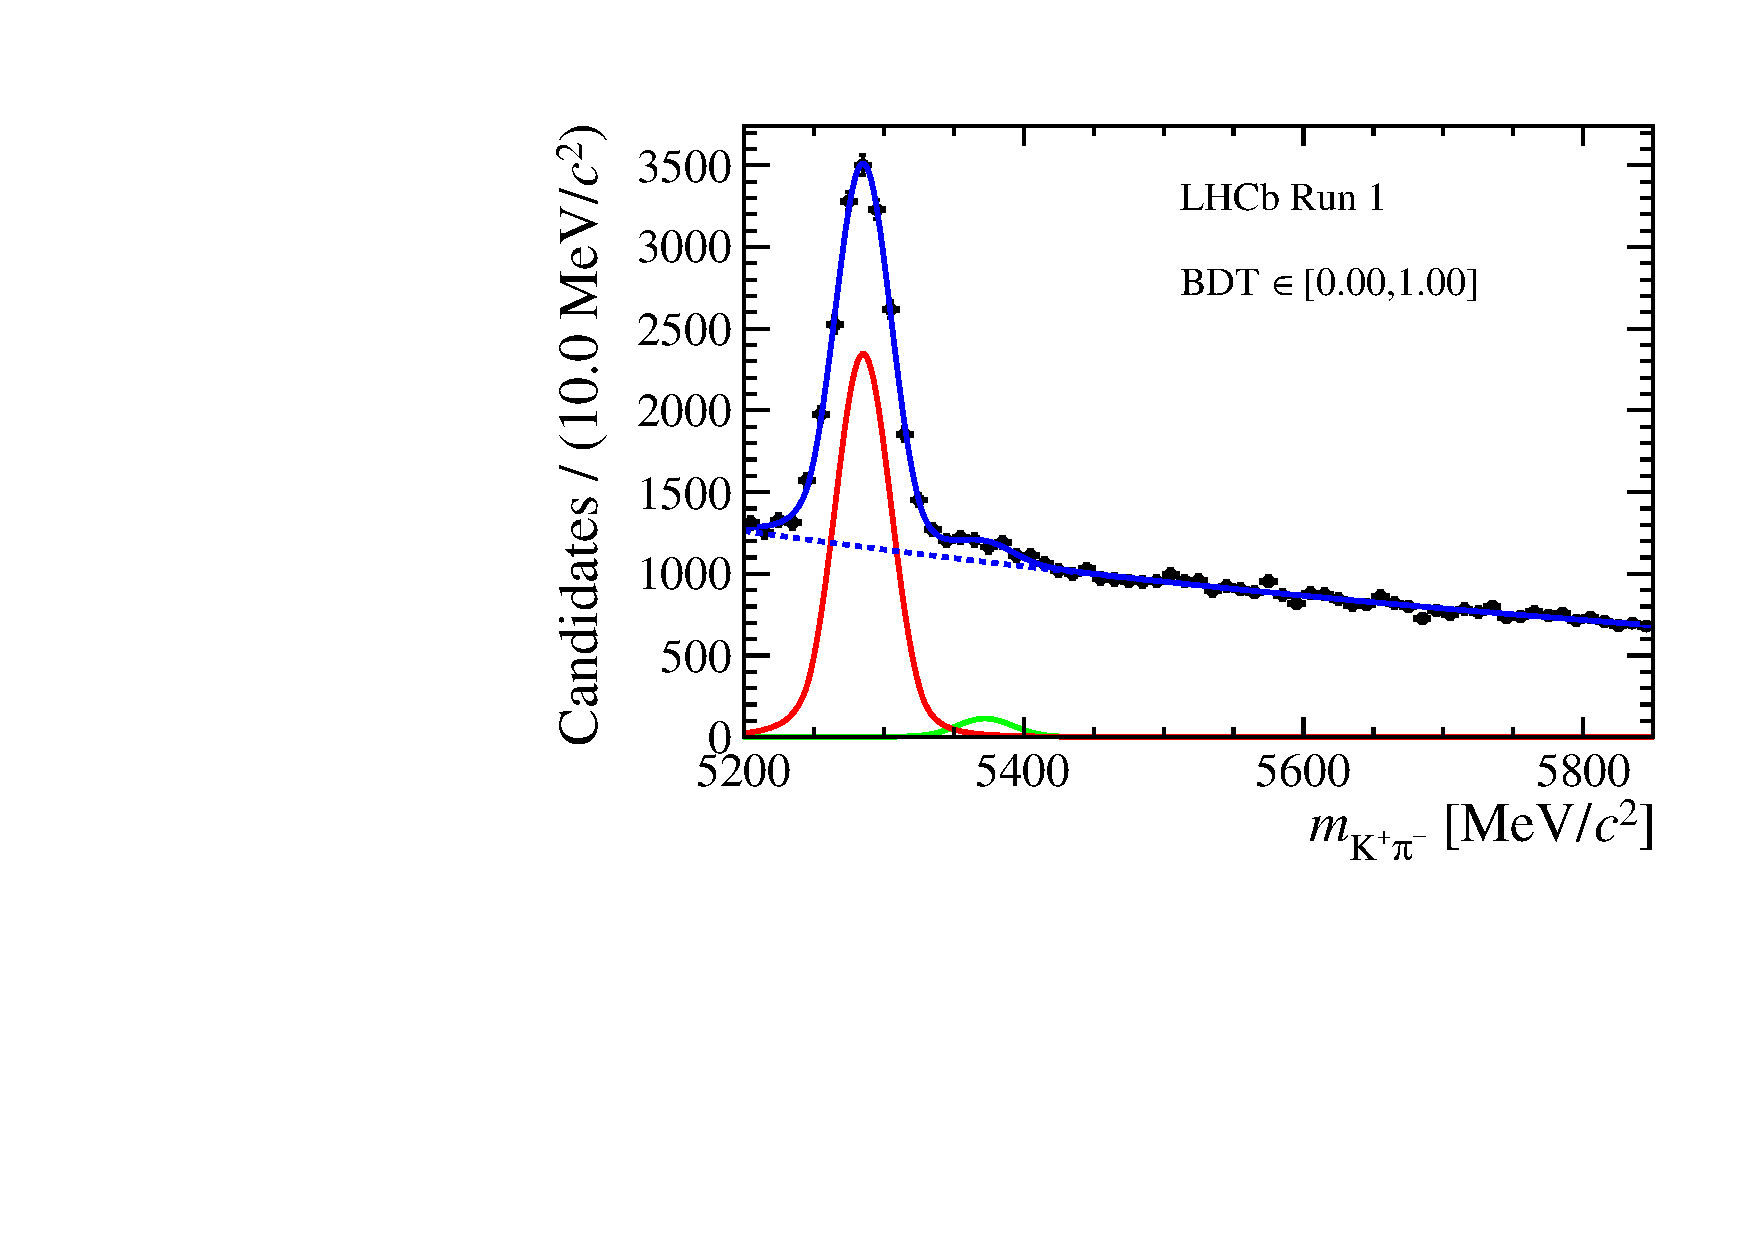
\includegraphics[width=  \textwidth]{./Figs/BFAnalysis/Bd2KPi_mass_RunI_BDTbinNone.pdf}
%        %\caption{ }
%       % \label{fig:BDTSsig}
%    \end{subfigure}
%   % ~ %add desired spacing between images, e. g. ~, \quad, \qquad, \hfill etc. 
%      %(or a blank line to force the subfigure onto a new line)
%    \begin{subfigure}[b]{0.48\textwidth}
%       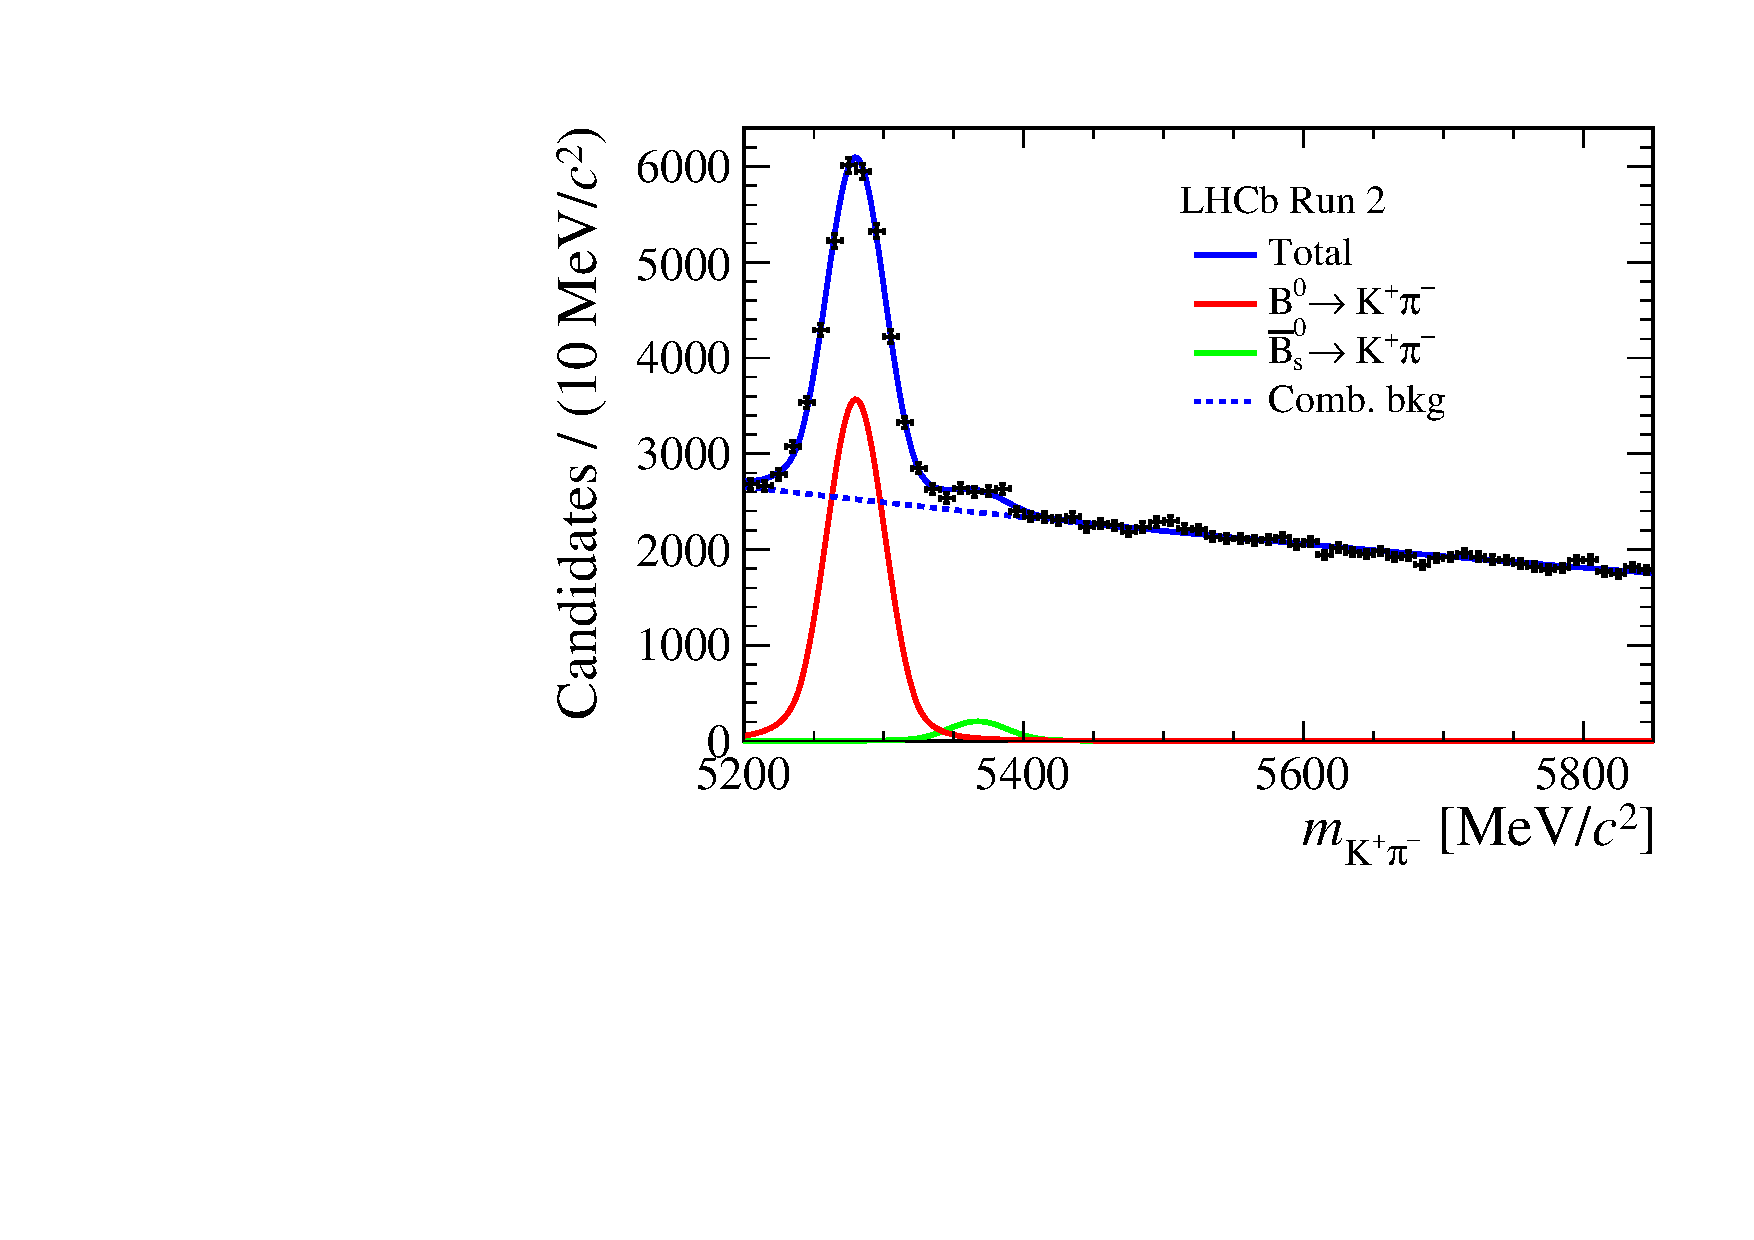
\includegraphics[width=\textwidth]{./Figs/BFAnalysis/Bd2KPi_mass_RunII_BDTbinNone.pdf}
%      %  \caption{ }
%     %   \label{fig:BDTSbkg}
%   \end{subfigure}
%    \caption{Mass fit to measure \bdkpi yield for the normalisation for Run 1 (left) and Run 2 (right) data. The total \pdf is made up of components for \bdkpi and \bskpi decays and combinatorial background.}
%    \label{fig:Bdkpiyield}
%\end{figure}



\begin{figure}[tbp]
    \centering
   %\begin{subfigure}[b]{0.48\textwidth}
        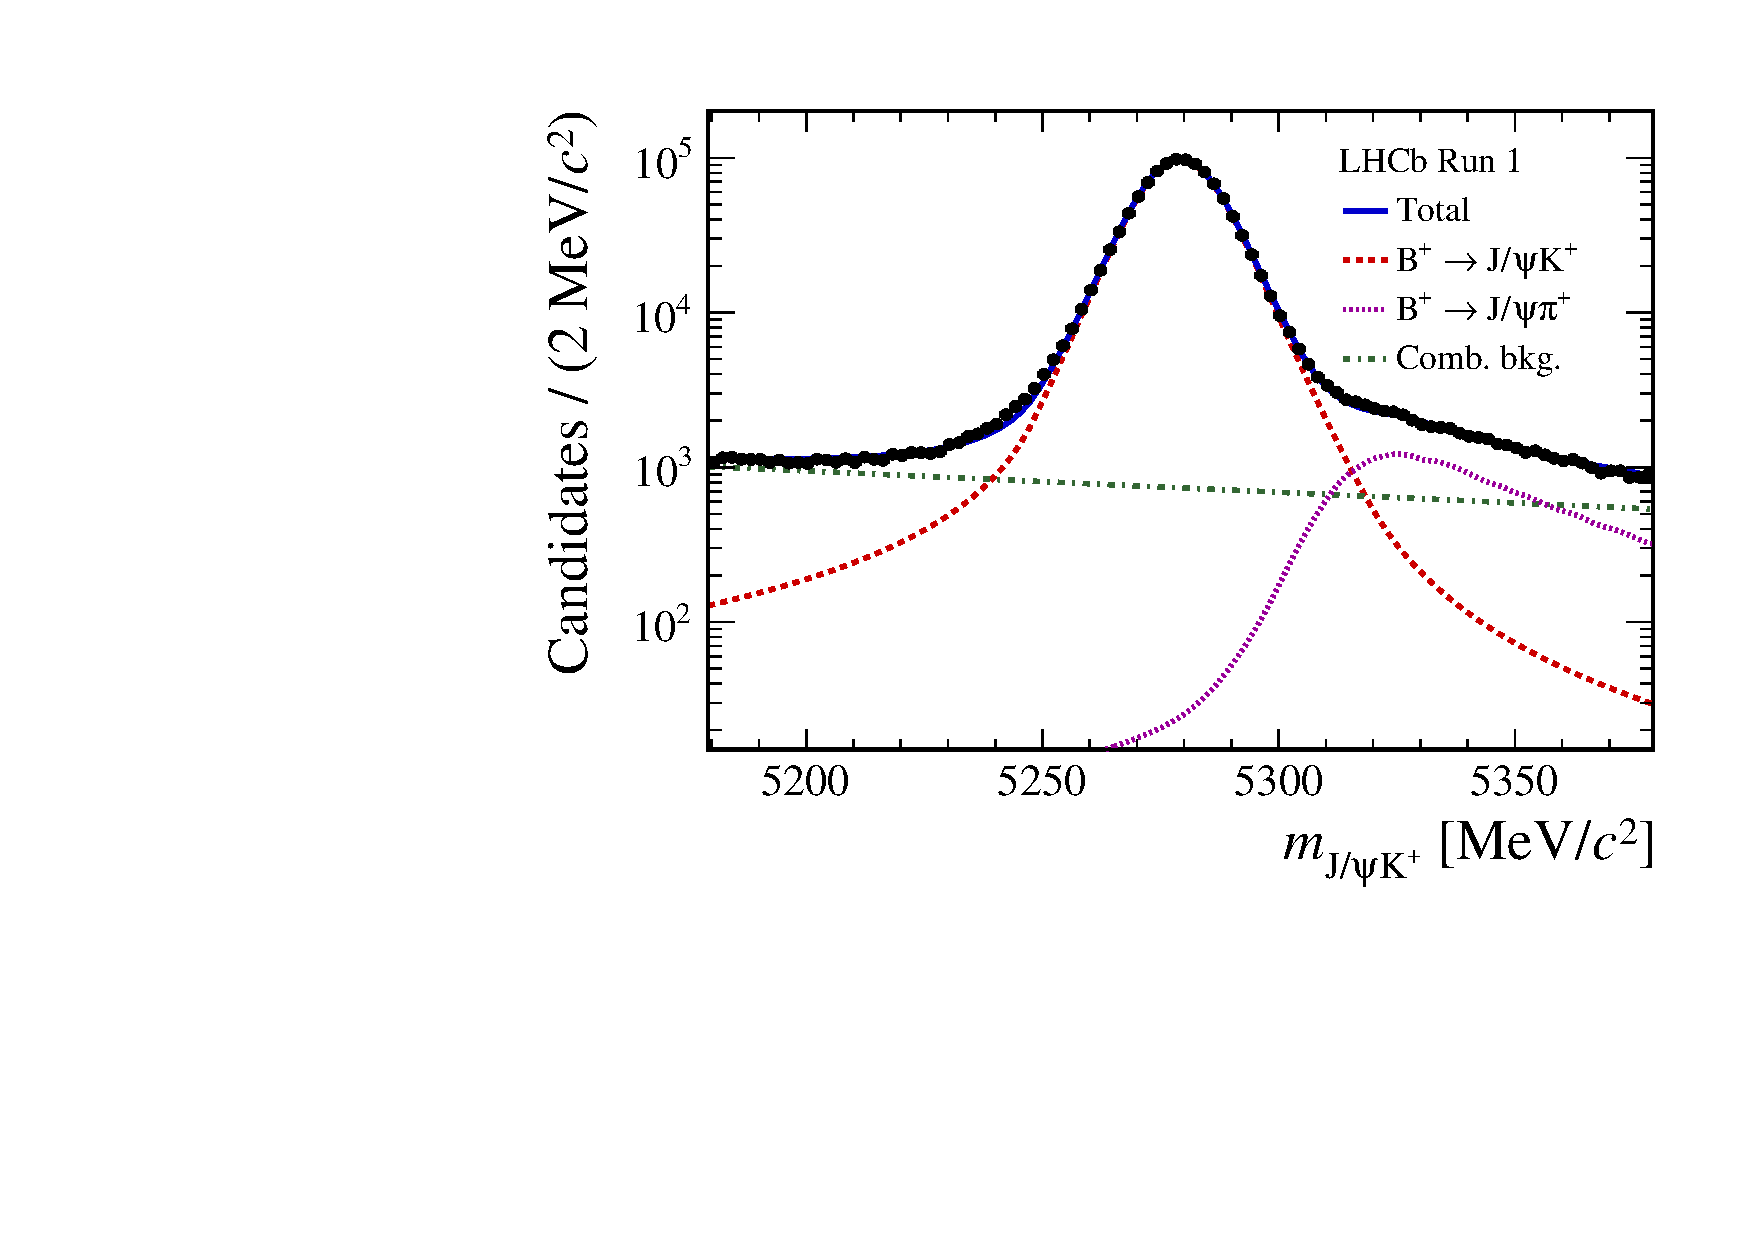
\includegraphics[width=  0.49\textwidth]{./Figs/BFAnalysis/BuJpsiK_Run1.pdf}
        %\caption{ }
       % \label{fig:BDTSsig}
   % \end{subfigure}
   % ~ %add desired spacing between images, e. g. ~, \quad, \qquad, \hfill etc. 
      %(or a blank line to force the subfigure onto a new line)
  %  \begin{subfigure}[b]{0.48\textwidth}
       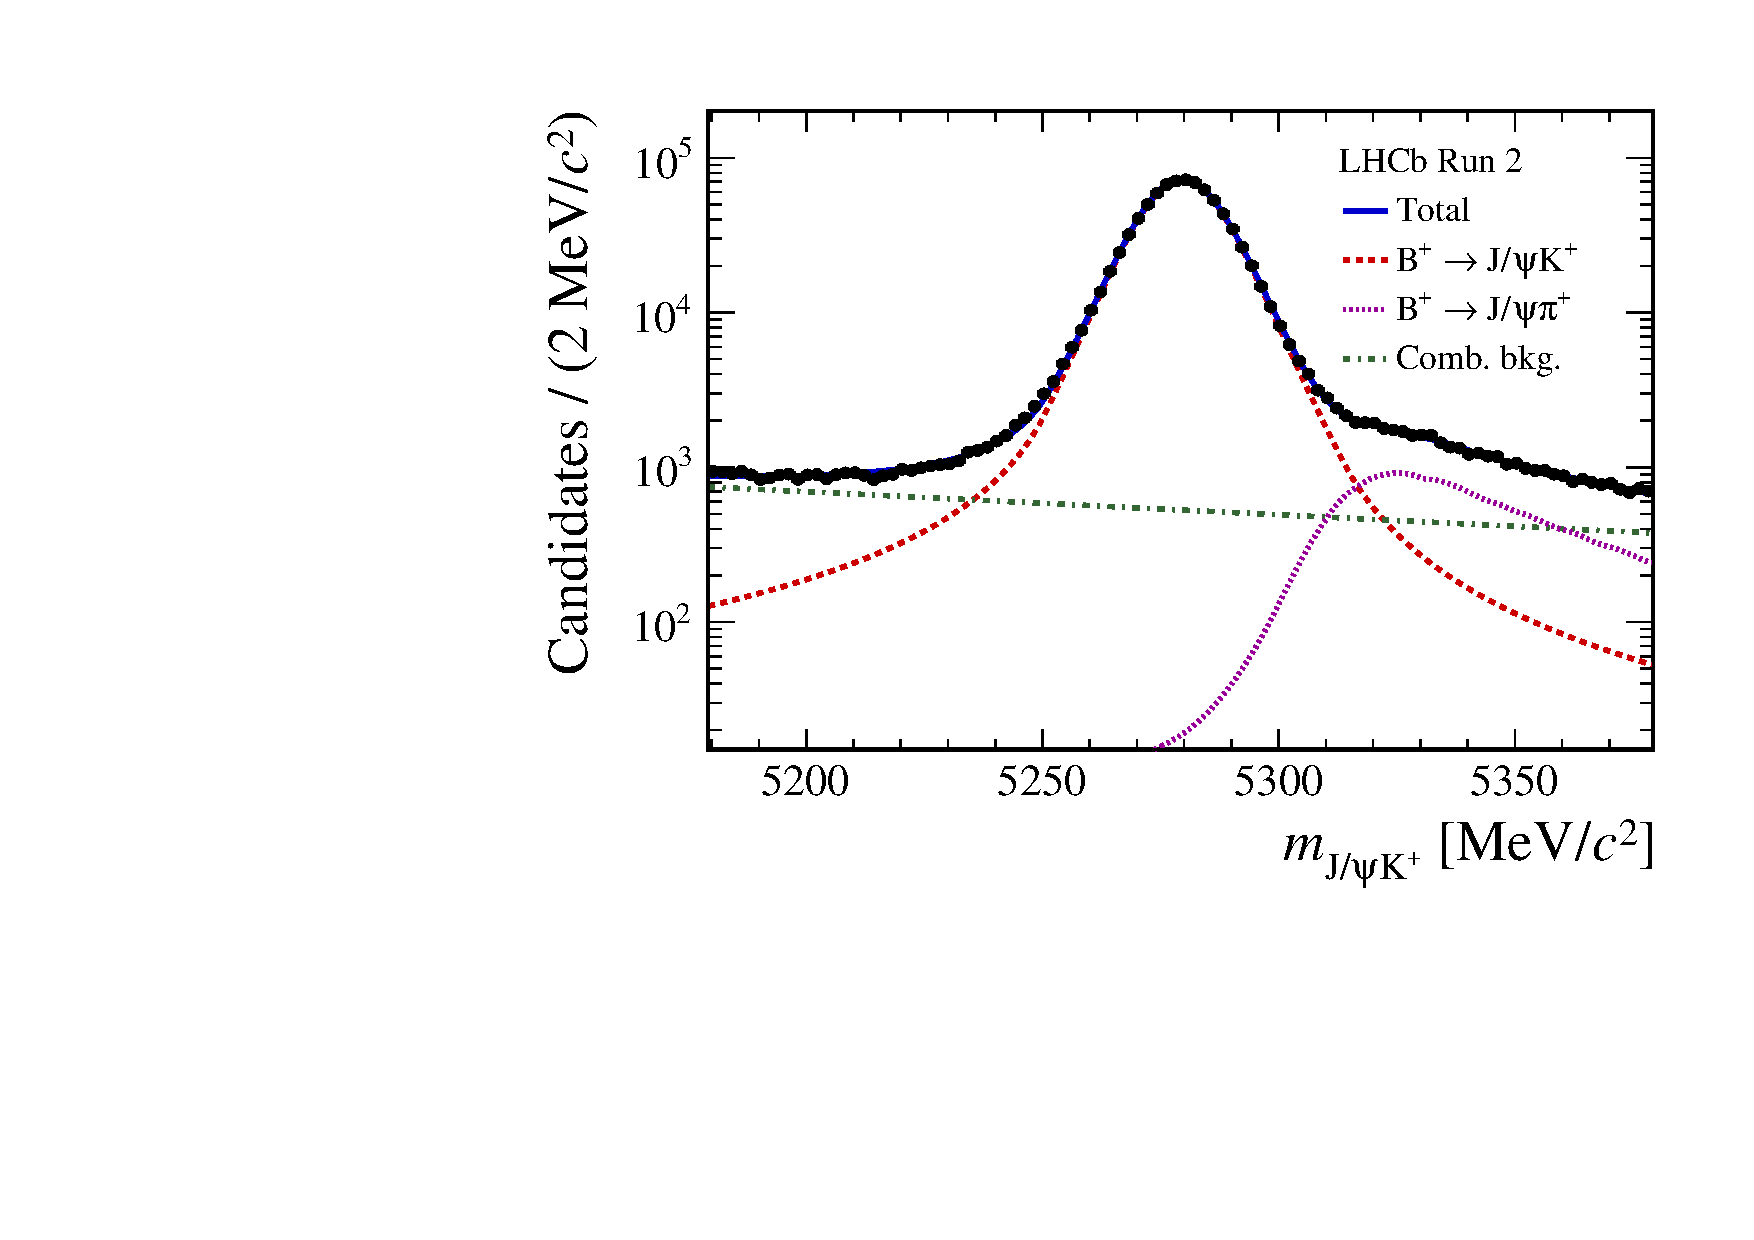
\includegraphics[width=0.49\textwidth]{./Figs/BFAnalysis/BuJpsiK_Run2.pdf}
      %  \caption{ }
     %   \label{fig:BDTSbkg}
 %  \end{subfigure}
    \caption{ Mass fit to measure the \bujpsik yield for the normalisation for Run 1 (left) and Run 2 (right) data. The total \pdf is made up of components of \bujpsik and $B^{+} \to J/\psi \pi^{+}$ decays and combinatorial background.}
    \label{fig:Bujpsikyield}
\end{figure}
\begin{figure}[tbp]
    \centering
  %\begin{subfigure}[b]{0.48\textwidth}
        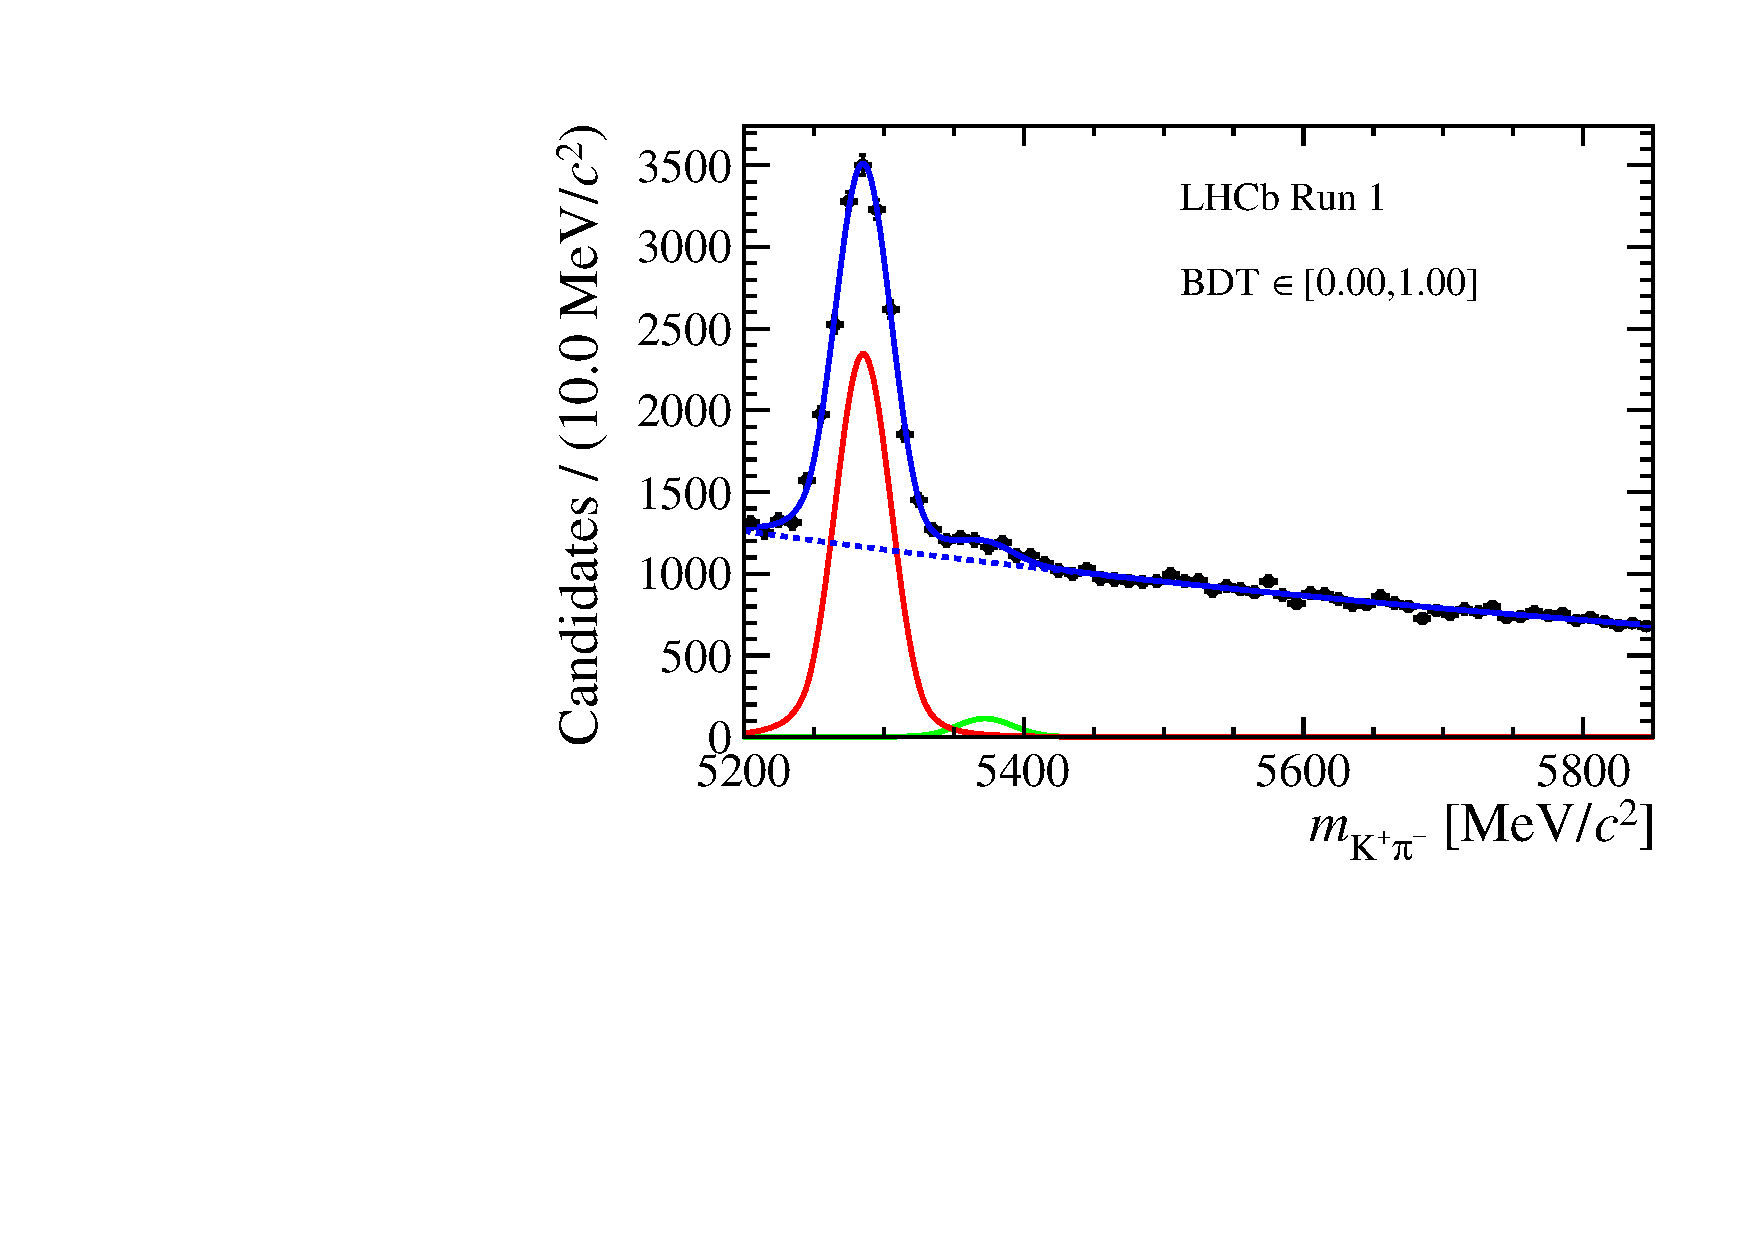
\includegraphics[width=  0.49\textwidth]{./Figs/BFAnalysis/Bd2KPi_mass_RunI_BDTbinNone.pdf}
        %\caption{ }                                                                                                                               
       % \label{fig:BDTSsig}                                                                                                                       
    %\end{subfigure}
   % ~ %add desired spacing between images, e. g. ~, \quad, \qquad, \hfill etc.                                                                    
      %(or a blank line to force the subfigure onto a new line)                                                                                    
    %\begin{subfigure}[b]{0.48\textwidth}
       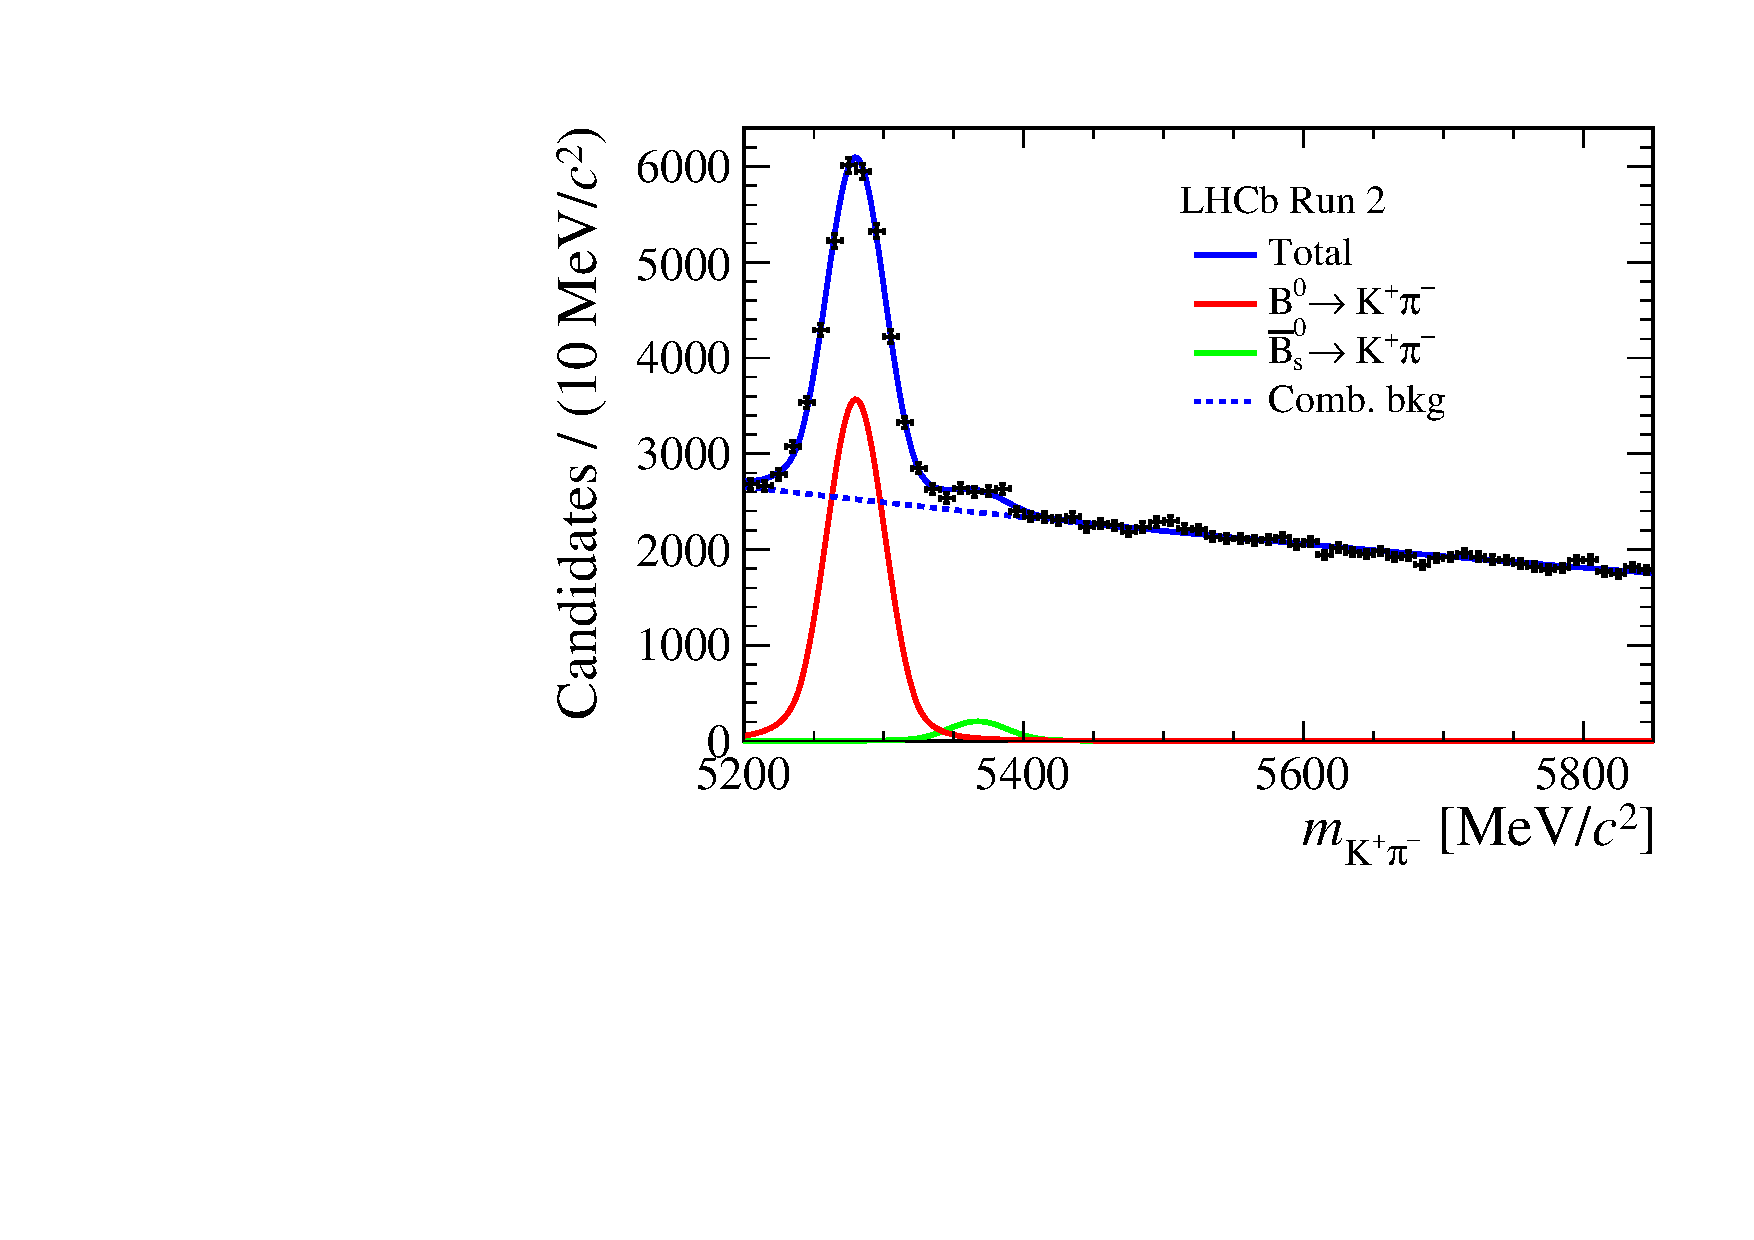
\includegraphics[width=0.49\textwidth]{./Figs/BFAnalysis/Bd2KPi_mass_RunII_BDTbinNone.pdf}
      %  \caption{ }                                                                                                                               
     %   \label{fig:BDTSbkg}                                                                                                                       
   %\end{subfigure}
    \caption{Mass fit to measure the \bdkpi yield for the normalisation for Run 1 (left) and Run 2 (right) data. The total \pdf is made up of component\
ts for \bdkpi and \bskpi decays and combinatorial background.}
    \label{fig:Bdkpiyield}
\end{figure}

\subsection{Efficiency ratio}
\label{sec:effratio}
The efficiency ratio in Equation~\ref{eq:BFnorm} is divided into several separate efficiency terms 
\begin{equation}
%\end{split}
\frac{\epsilon_{norm}}{\epsilon_{B^{0}_{(s)} \to \mu^{+} \mu^{-}}}  =  \frac{\epsilon^{Acc}_{norm}}{\epsilon^{Acc}_{B^{0}_{(s)} \to \mu^{+} \mu^{-}}} \cdot \frac{\epsilon^{RecSel|Acc}_{norm}}{\epsilon^{RecSel|Acc}_{B^{0}_{(s)} \to \mu^{+} \mu^{-}}} \cdot \frac{\epsilon^{Trig|RecSel}_{norm}}{\epsilon^{Trig|RecSel}_{B^{0}_{(s)} \to \mu^{+} \mu^{-}}},
%\end{split}
\label{eq:BFnormDetailed}
\end{equation}
%for the detector acceptance, $\epsilon^{Acc}$, reconstruction and selection efficiency, $\epsilon^{RecSel|Acc}$, and the trigger efficiency, $\epsilon^{Trig|RecSel}$. 
where $\epsilon^{Acc}$ is the detector acceptance efficiency, $\epsilon^{RecSel|Acc}$ the reconstruction and selection efficiency given the detector efficiency, and $\epsilon^{Trig|RecSel}$ the trigger efficiency given the reconstruction and selection efficiency. 

The detector acceptance efficiency gives the efficiency for the decay products to be within the LHCb detector angular acceptance. This efficiency is evaluated on simulated decays for decay products that fall within the range [10,400] mrad in both $x$ and $y$ directions. The range is chosen to be slightly larger than the detector acceptance so that particles recovered by the magnetic field are included. To keep this efficiency similar for \bmumu and \bdkpi decays, the hadrons from \bdkpi decays are required to be within the muon detector acceptance. 

The reconstruction and selection efficiency of decays within the detector acceptance is evaluated from a combination of information from data and simulated decays. Similar to the fraction of \bsmumu in each BDT bin, a correction is applied for the lifetime used in simulated \bsmumu decays assuming \ADG = +1. 

The trigger efficiencies for decays passing the reconstruction and selection are evaluated for each decay by data driven methods as described in~\cite{Tolk:2148631, Tolk:1557354}. % , Tolk:2148631}. 

The efficiencies are calculated for \bsmumu, \bdmumu, \bdkpi and \bujpsik separately to account for differences between the decay kinematics. The ratio of efficiencies between signal and normalisation channels used in the normalisation parameters ensures that systematic uncertainties arising from the use of simulated decays cancel out and will not affect the measurements of the \bmumu branching fractions.

\subsection{Hadronisation factors}
\label{hadronfact}
The normalisation factors depend on the hadronisation factors, $f_{u}, f_{s}, f_{d}$, that give the fraction of $b\bar{b}$ pairs that produce $B^{\pm}$, \bd or $\overline{B}^{0}$ and \bs or $\overline{B}^{0}_{s}$ mesons. %probability of a $b$ or $\bar{b}$ quark to form a $B^{+}$, \bs or \bd, respectively. 
The factors $f_{d}$ and $f_{u}$ are equal to good approximation, therefore the \bdmumu branching fraction does not depend on any hadronisation factors. For the \bsmumu decay the ratio $f_{s}/f_{d}$ is used in the normalisation, since $f_{d} = f_{u}$. This ratio has been measured at LHCb for $pp$ collisions at $\sqrt{s}$ = 7~TeV~\cite{LHCb-CONF-2013-011}. The stability of this ratio at different centre-of-mass energies was tested using the ratio of \bsjpsiphi and \bujpsik decays at 8 and 13 \tev relative to their ratio at 7~\tev. %The reconstruction, selection and trigger efficiencies were corrected for in the ratios. 
The ratios are stable across the different collision energies and $f_{s}/f_{d}$ is assumed to be identical for $\sqrt{s}$ = 8 TeV. For Run~2, the $f_{s}/f_{d}$ ratio is modified due to a small relative production difference in \bsjpsiphi and \bujpsik decays observed for Run~2 compared to Run~1. 
The uncertainty on the hadronisation factor ratio contributes the largest systematic uncertainty to the \bsmumu branching fraction. 

Alternatively, the \bsmumu \BF could be normalised using a different \bs decay, such as \bsjpsiphi. However the precision of the measured branching fractions and abundance of such decays is not high enough at present to provide a lower overall uncertainty on the measured branching fraction.

\subsection{Normalisation parameters}
\label{normparams}
The yields, efficiencies and hadronisation factors are combined to produce separate normalisation factors for each year of data taking and each normalisation channel. The consistency of the efficiencies and yields for each normalisation channel are checked for each year by comparing the ratios $\mathcal{B}$(\bdkpi)/$\mathcal{B}$(\bujpsik) and $\mathcal{B}$(\bujpsik)/$\mathcal{B}$(\bsjpsiphi) with the average of previously measured values of these quantities in reference~\cite{Olive:2016xmw}. The efficiencies and yields are consistent with the measured values for these decays. 


The yearly normalisation factors are combined for each channel to produce the overall normalisation factors for Run 1 and Run 2, taking into account correlations between the parameters. A weighted average of the normalisation factors for \bdkpi and \bujpsik decays are used to produce the overall normalisation factors for Run 1 and Run 2 as shown in Table~\ref{tab:normparams}.

\begin{table}[tb]
\begin{center}
\begin{tabular}{lcc}
\toprule \toprule
Normalisation Parameters & Run 1 & Run 2 \\ \midrule
$\alpha_{d} \times 10^{11}$ & 2.88 $\pm$ 0.10 & 3.52 $\pm$ 0.16 \\ %Why are they so differe  
$\alpha_{s} \times 10^{10}$ & 1.07 $\pm$ 0.07 & 1.31$ \pm$ 0.10 \\
\bottomrule \bottomrule
\end{tabular}
\vspace{0.7cm}
\caption{Normalisation parameters for \bsmumu and \bdmumu for Run~1 and Run~2.}
\label{tab:normparams}
\end{center}
\vspace{-1.0cm}
\end{table}


\section{Results}
\label{sec:BFResults}

%As described in Section~\ref{sec:BFAnalysisStrategy} 
The \bdmumu and \bsmumu branching fractions are measured by a simultaneous fit to the dimuon invariant mass distribution across eight categories: Run~1, Run~2 and four BDT bins, as described in Section~\ref{sec:BFAnalysisStrategy}. % for each Run.
The fit results are shown in Figure~\ref{fig:BFfit}.

\begin{figure}[tbp]
    \centering
    \begin{subfigure}[b]{0.48\textwidth}
        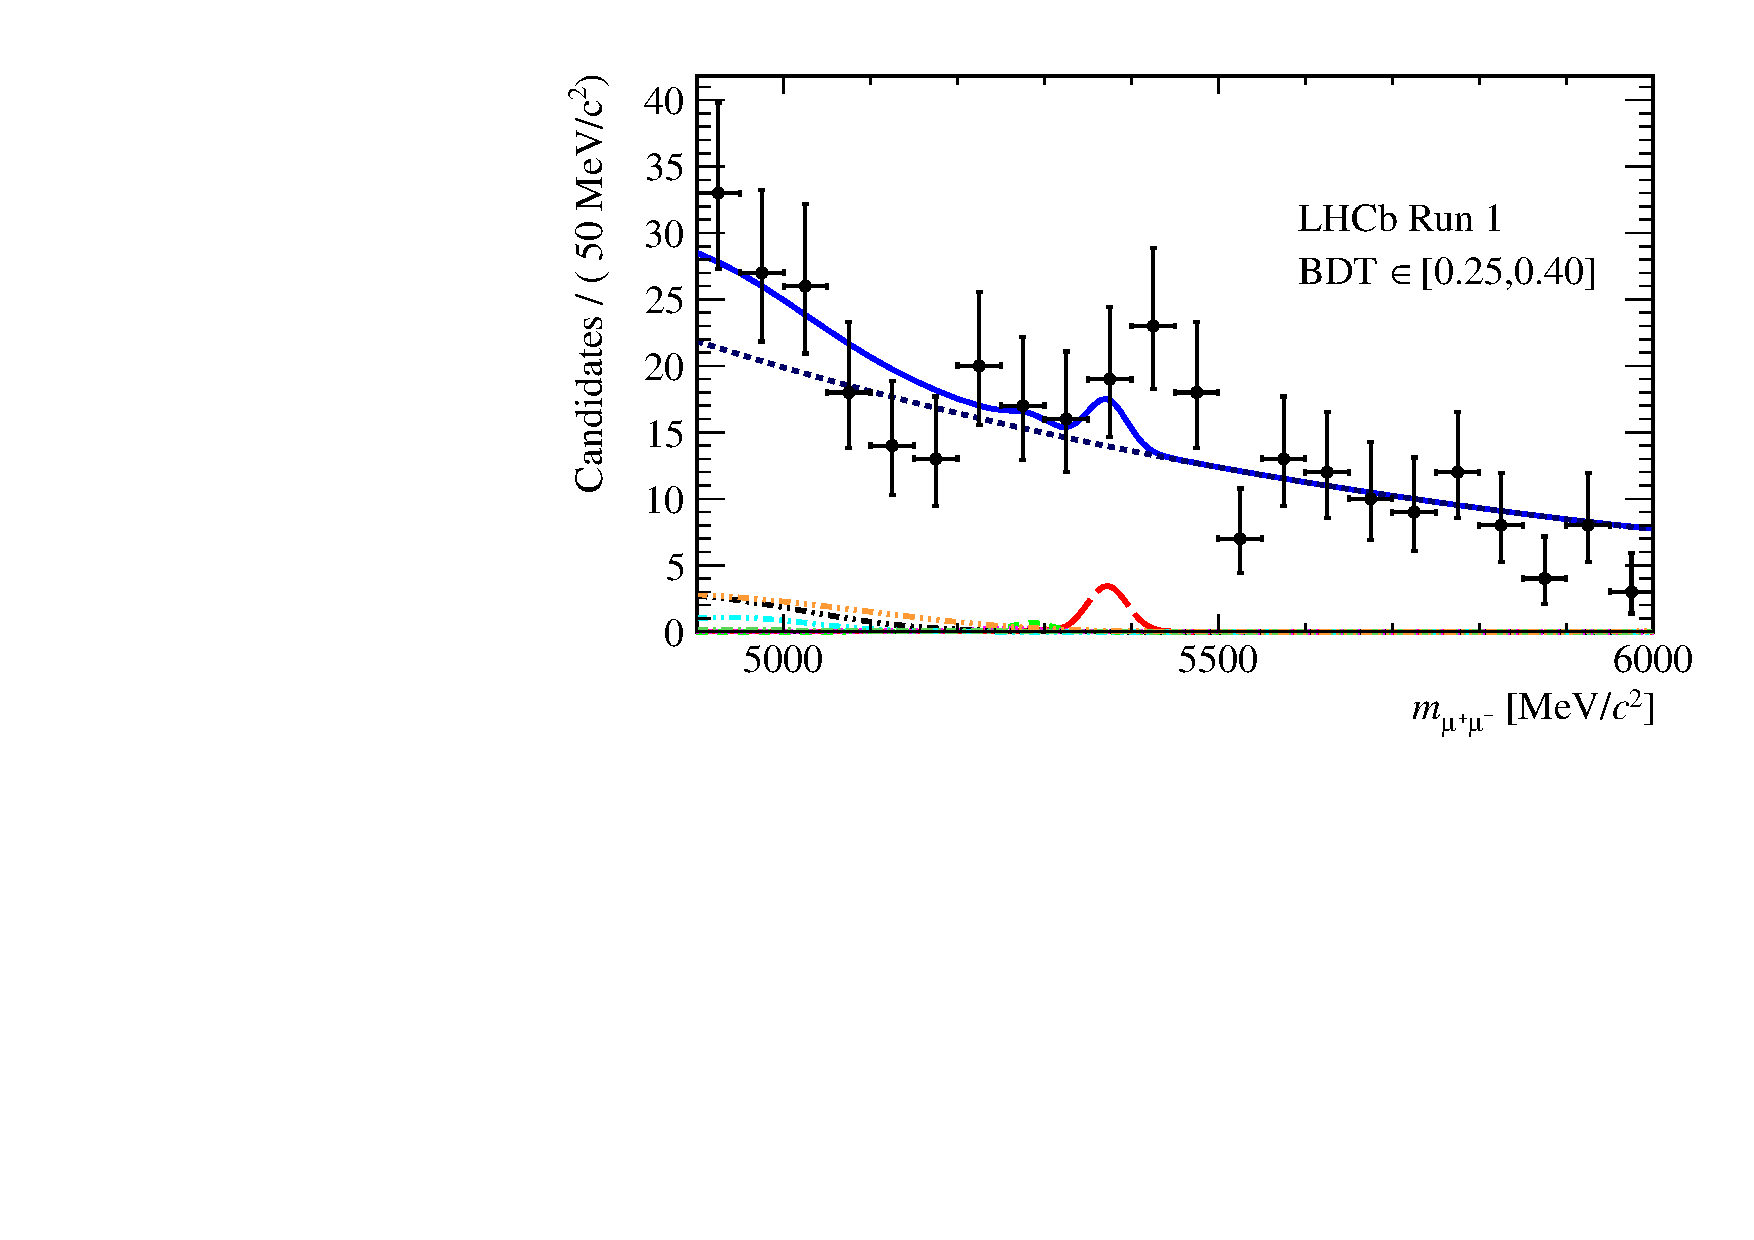
\includegraphics[width=\textwidth]{./Figs/BFAnalysis/Fig17a.pdf}
    \end{subfigure}
    ~ %add desired spacing between images, e. g. ~, \quad, \qquad, \hfill etc.                                       
      %(or a blank line to force the subfigure onto a new line)                                                      
    \begin{subfigure}[b]{0.48\textwidth}
       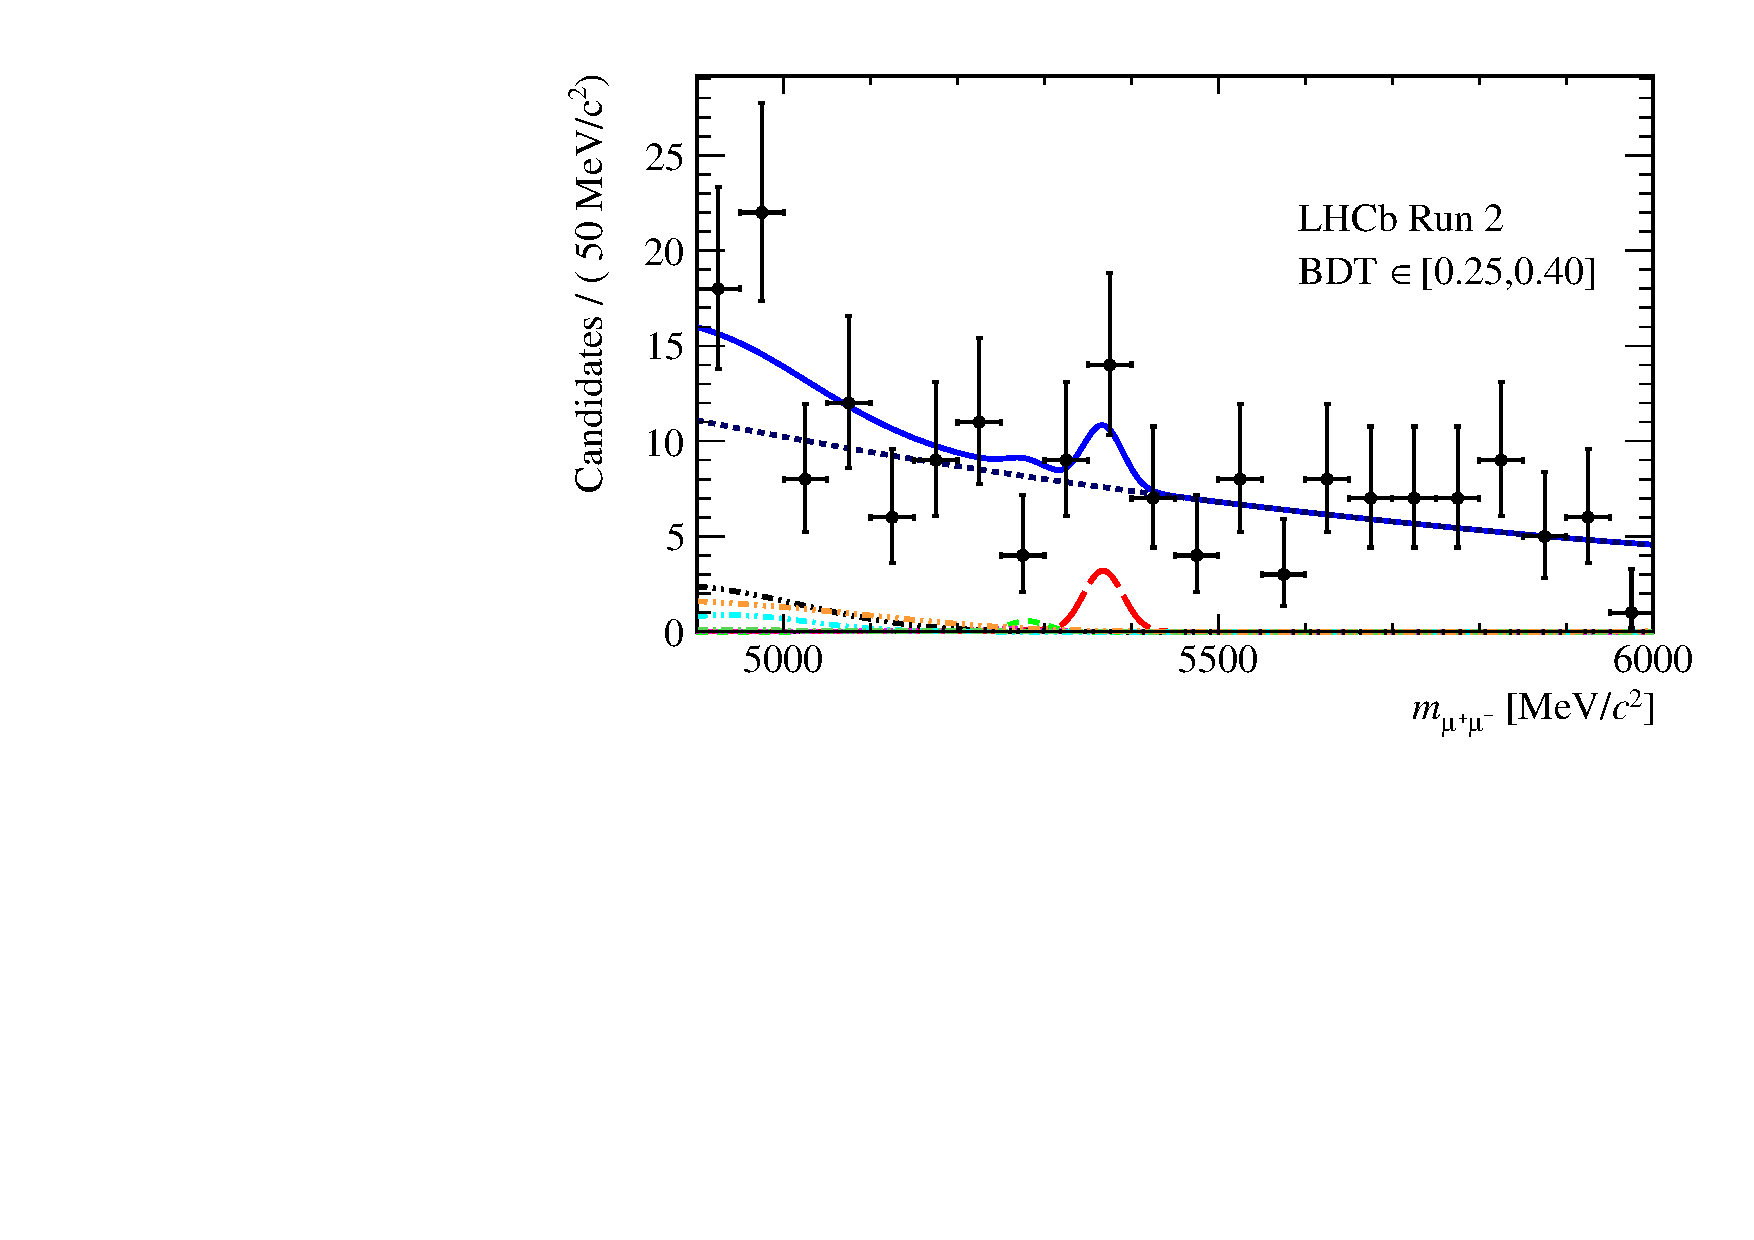
\includegraphics[width=\textwidth]{./Figs/BFAnalysis/Fig17e.pdf}
    \end{subfigure}
    \begin{subfigure}[b]{0.48\textwidth}
        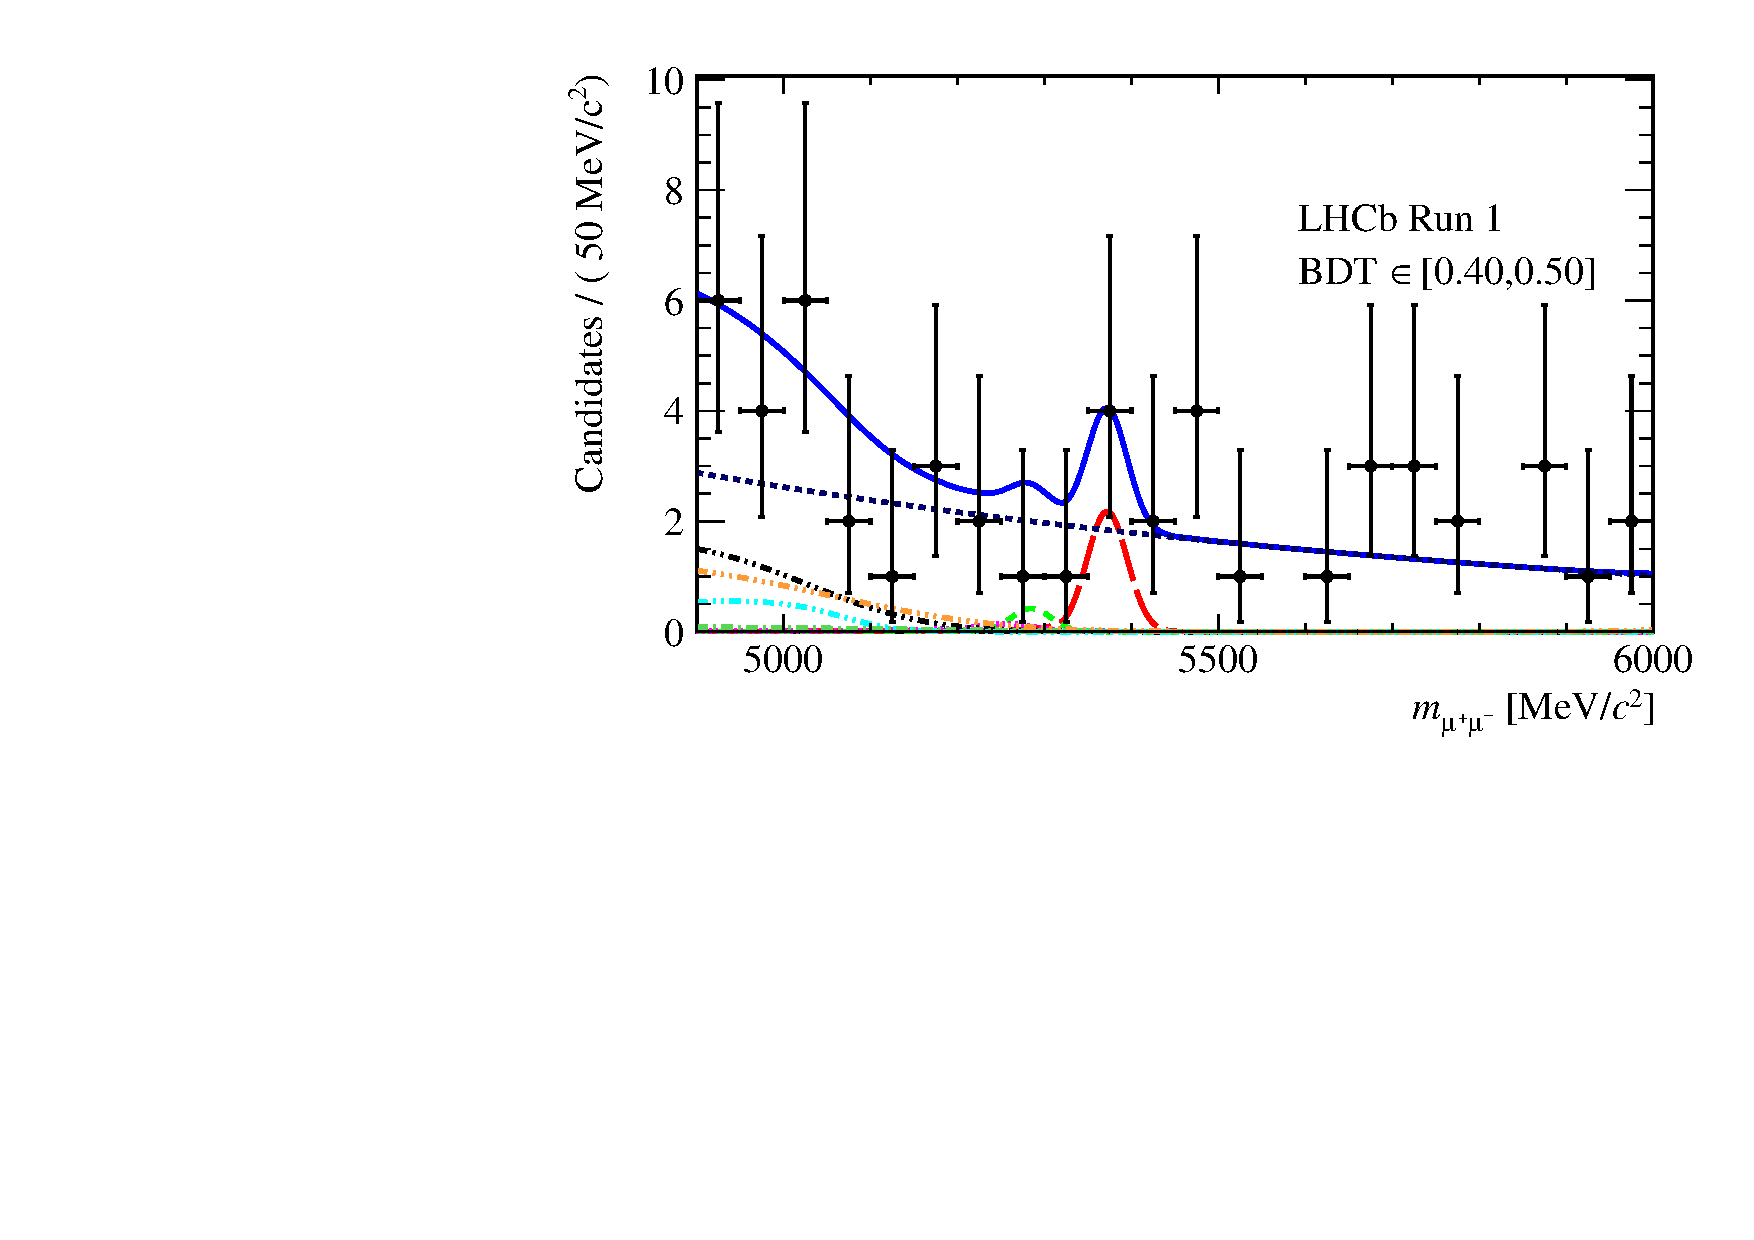
\includegraphics[width=\textwidth]{./Figs/BFAnalysis/Fig17b.pdf}
    \end{subfigure}
    ~ %add desired spacing between images, e. g. ~, \quad, \qquad, \hfill etc.                                       
      %(or a blank line to force the subfigure onto a new line)                                                      
    \begin{subfigure}[b]{0.48\textwidth}
       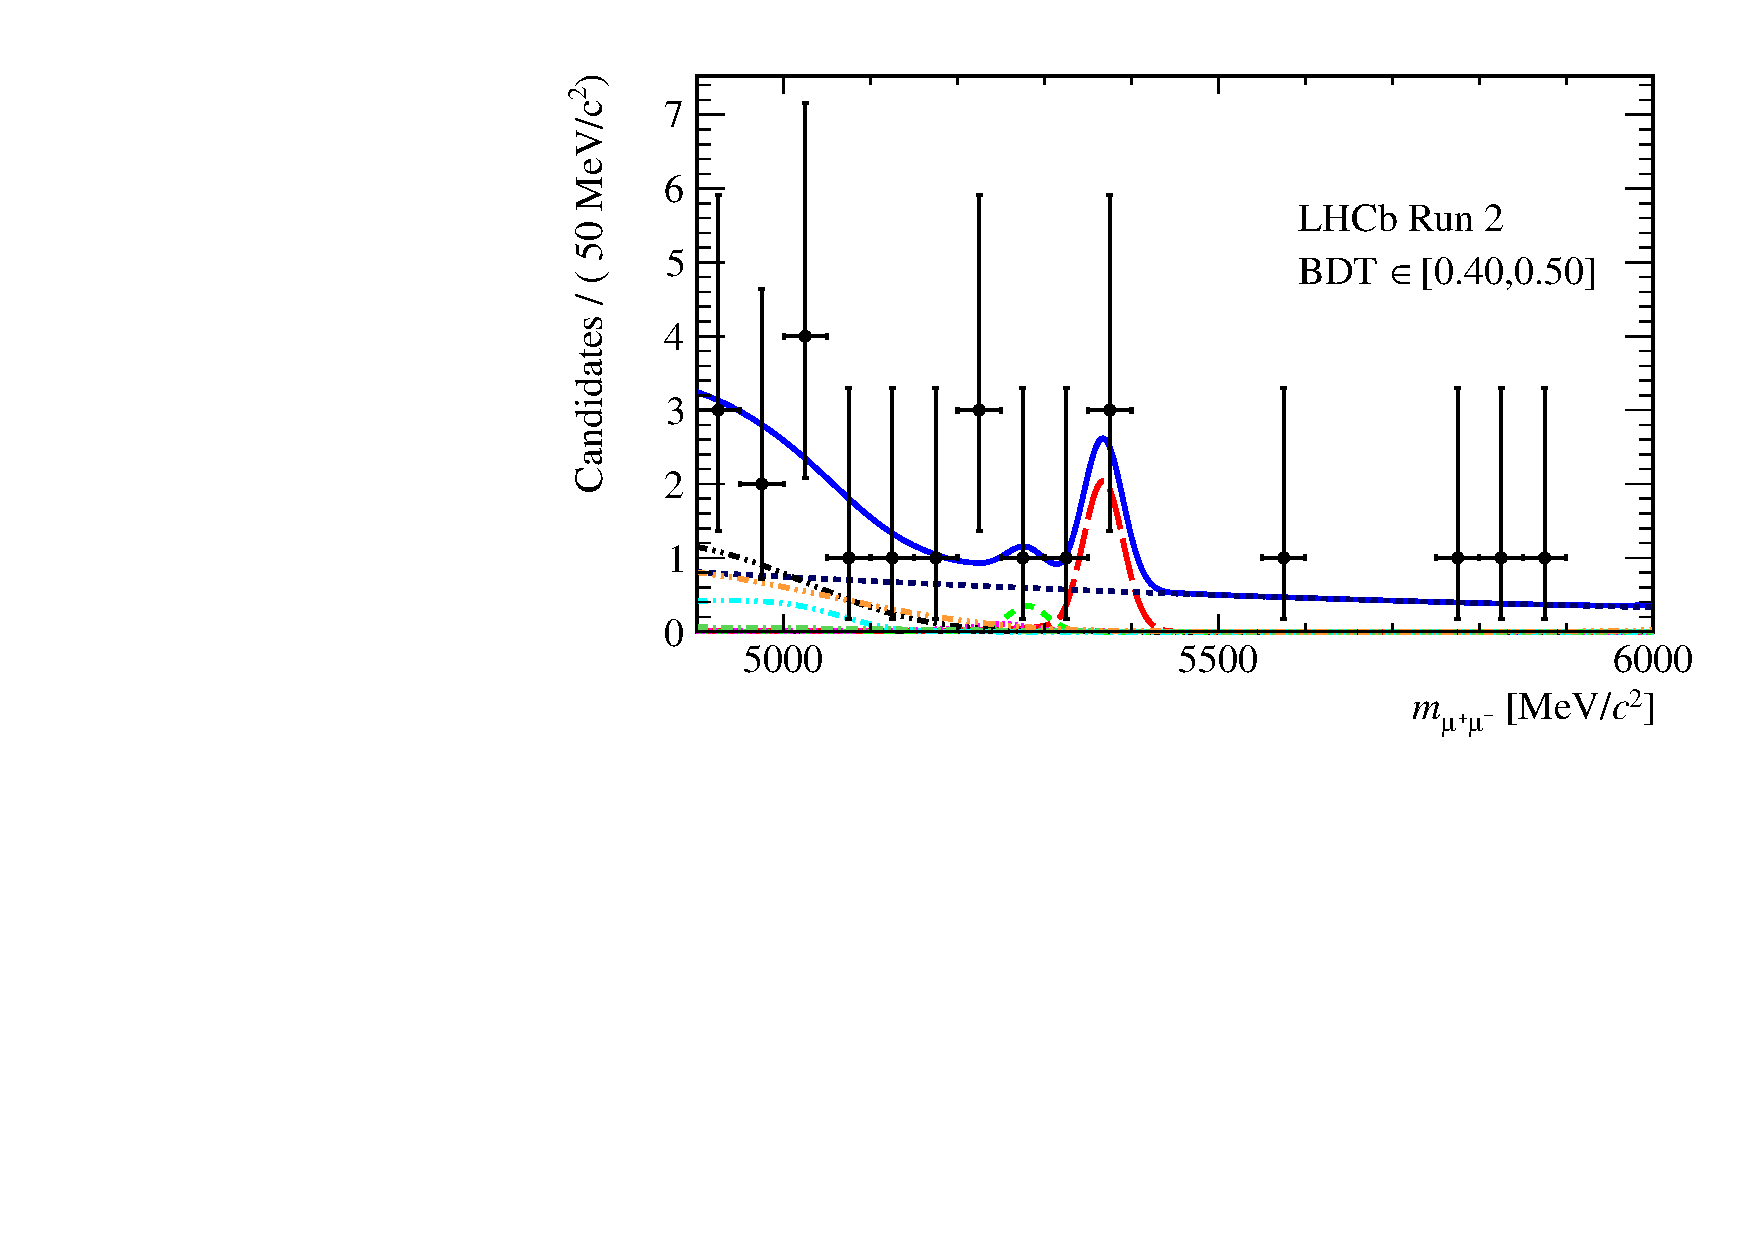
\includegraphics[width=\textwidth]{./Figs/BFAnalysis/Fig17f.pdf}
    \end{subfigure}
    ~
      \begin{subfigure}[b]{0.48\textwidth}
        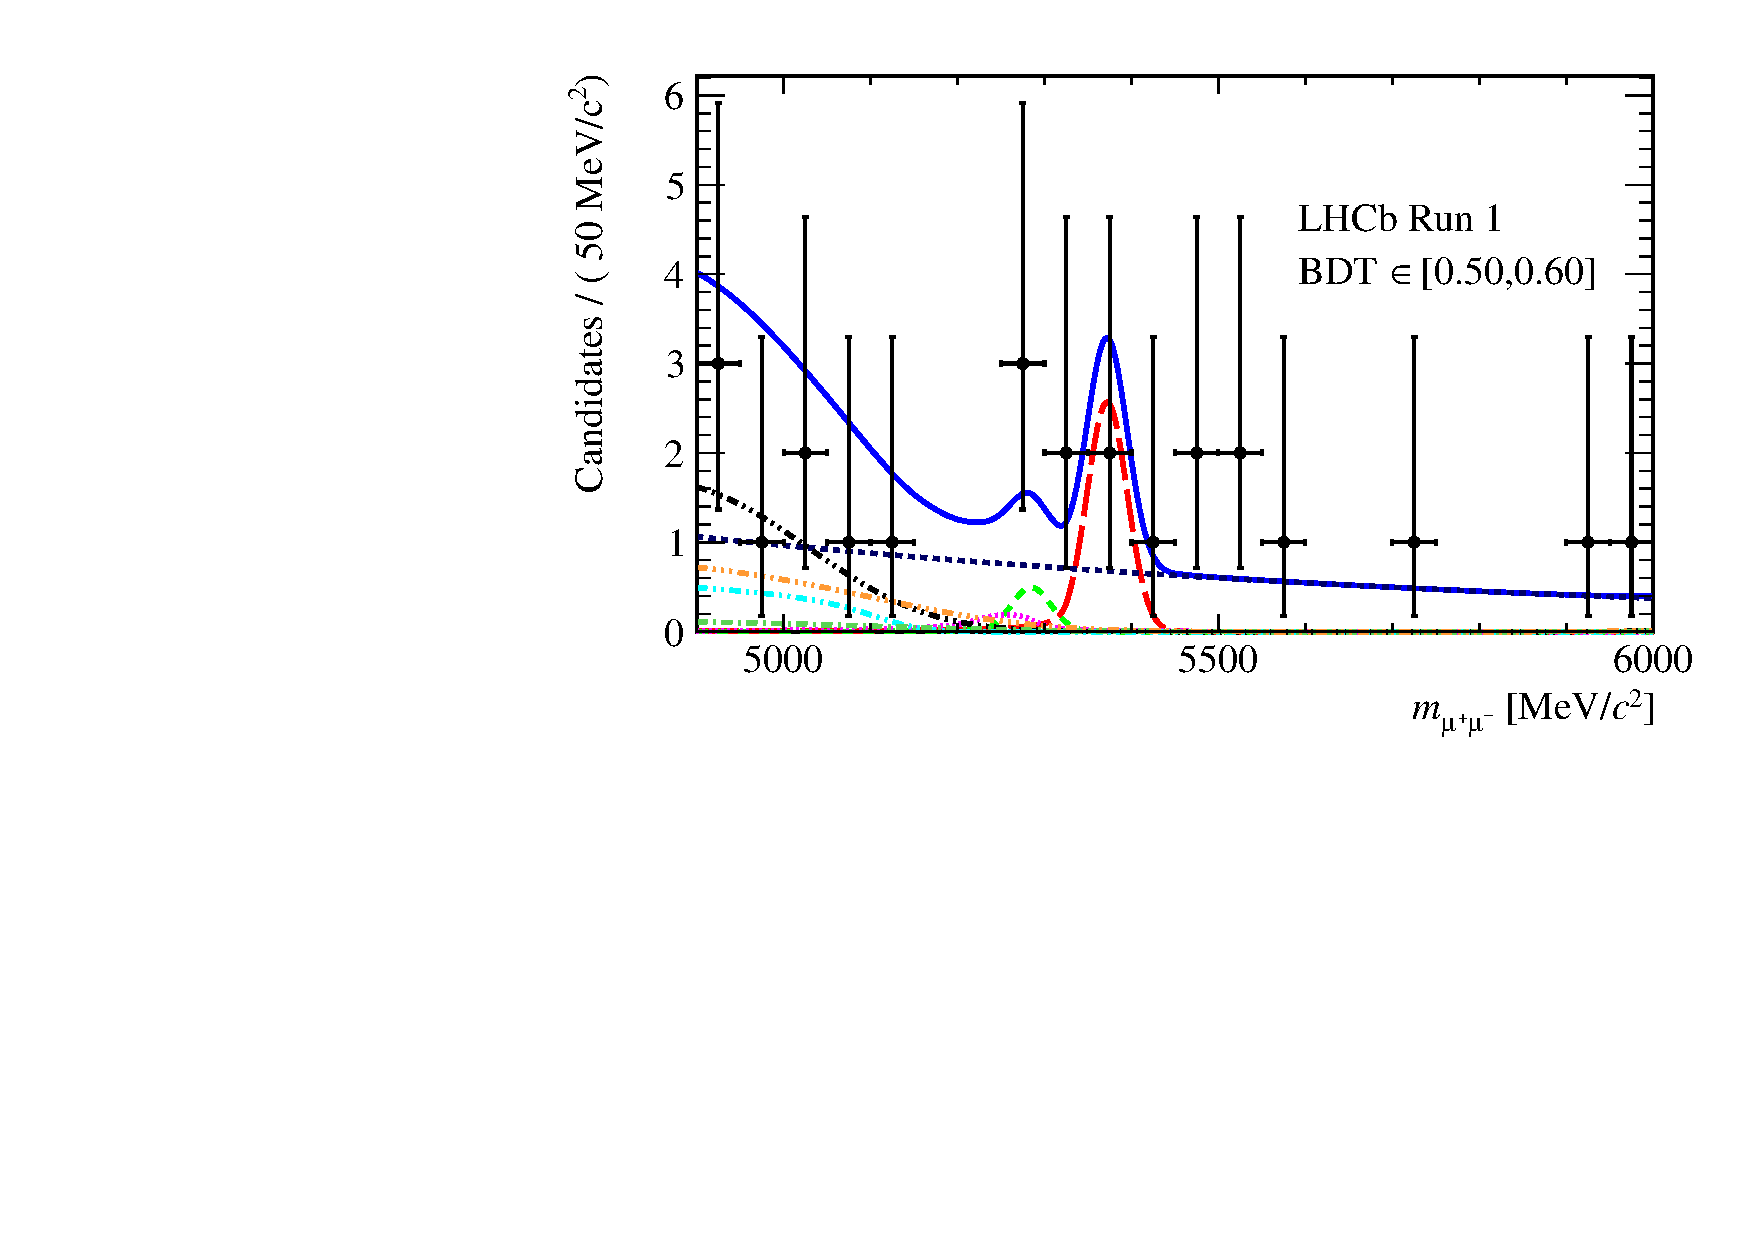
\includegraphics[width=\textwidth]{./Figs/BFAnalysis/Fig17c.pdf}
    \end{subfigure}
    ~ %add desired spacing between images, e. g. ~, \quad, \qquad, \hfill etc.                                       
      %(or a blank line to force the subfigure onto a new line)                                                      
    \begin{subfigure}[b]{0.48\textwidth}
       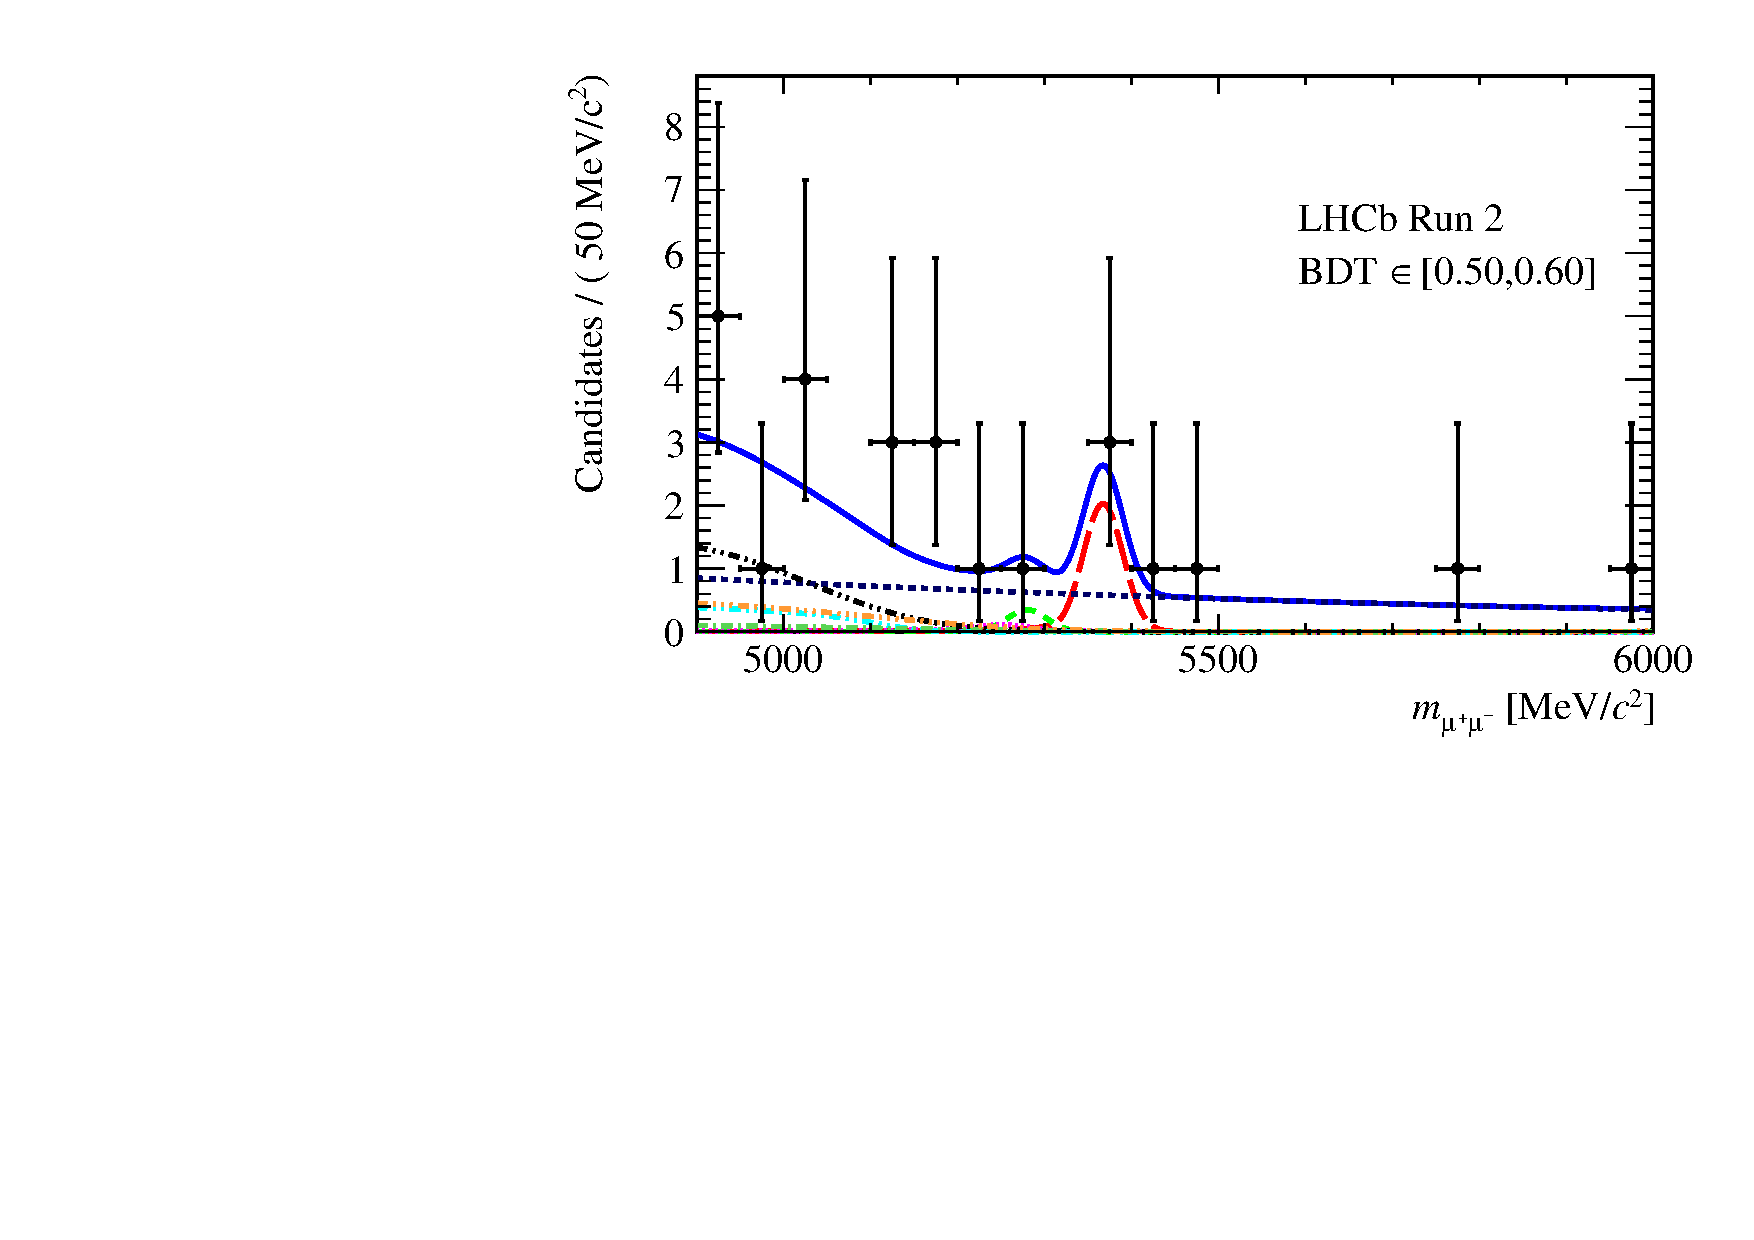
\includegraphics[width=\textwidth]{./Figs/BFAnalysis/Fig17g.pdf}
    \end{subfigure}
    \begin{subfigure}[b]{0.48\textwidth}
        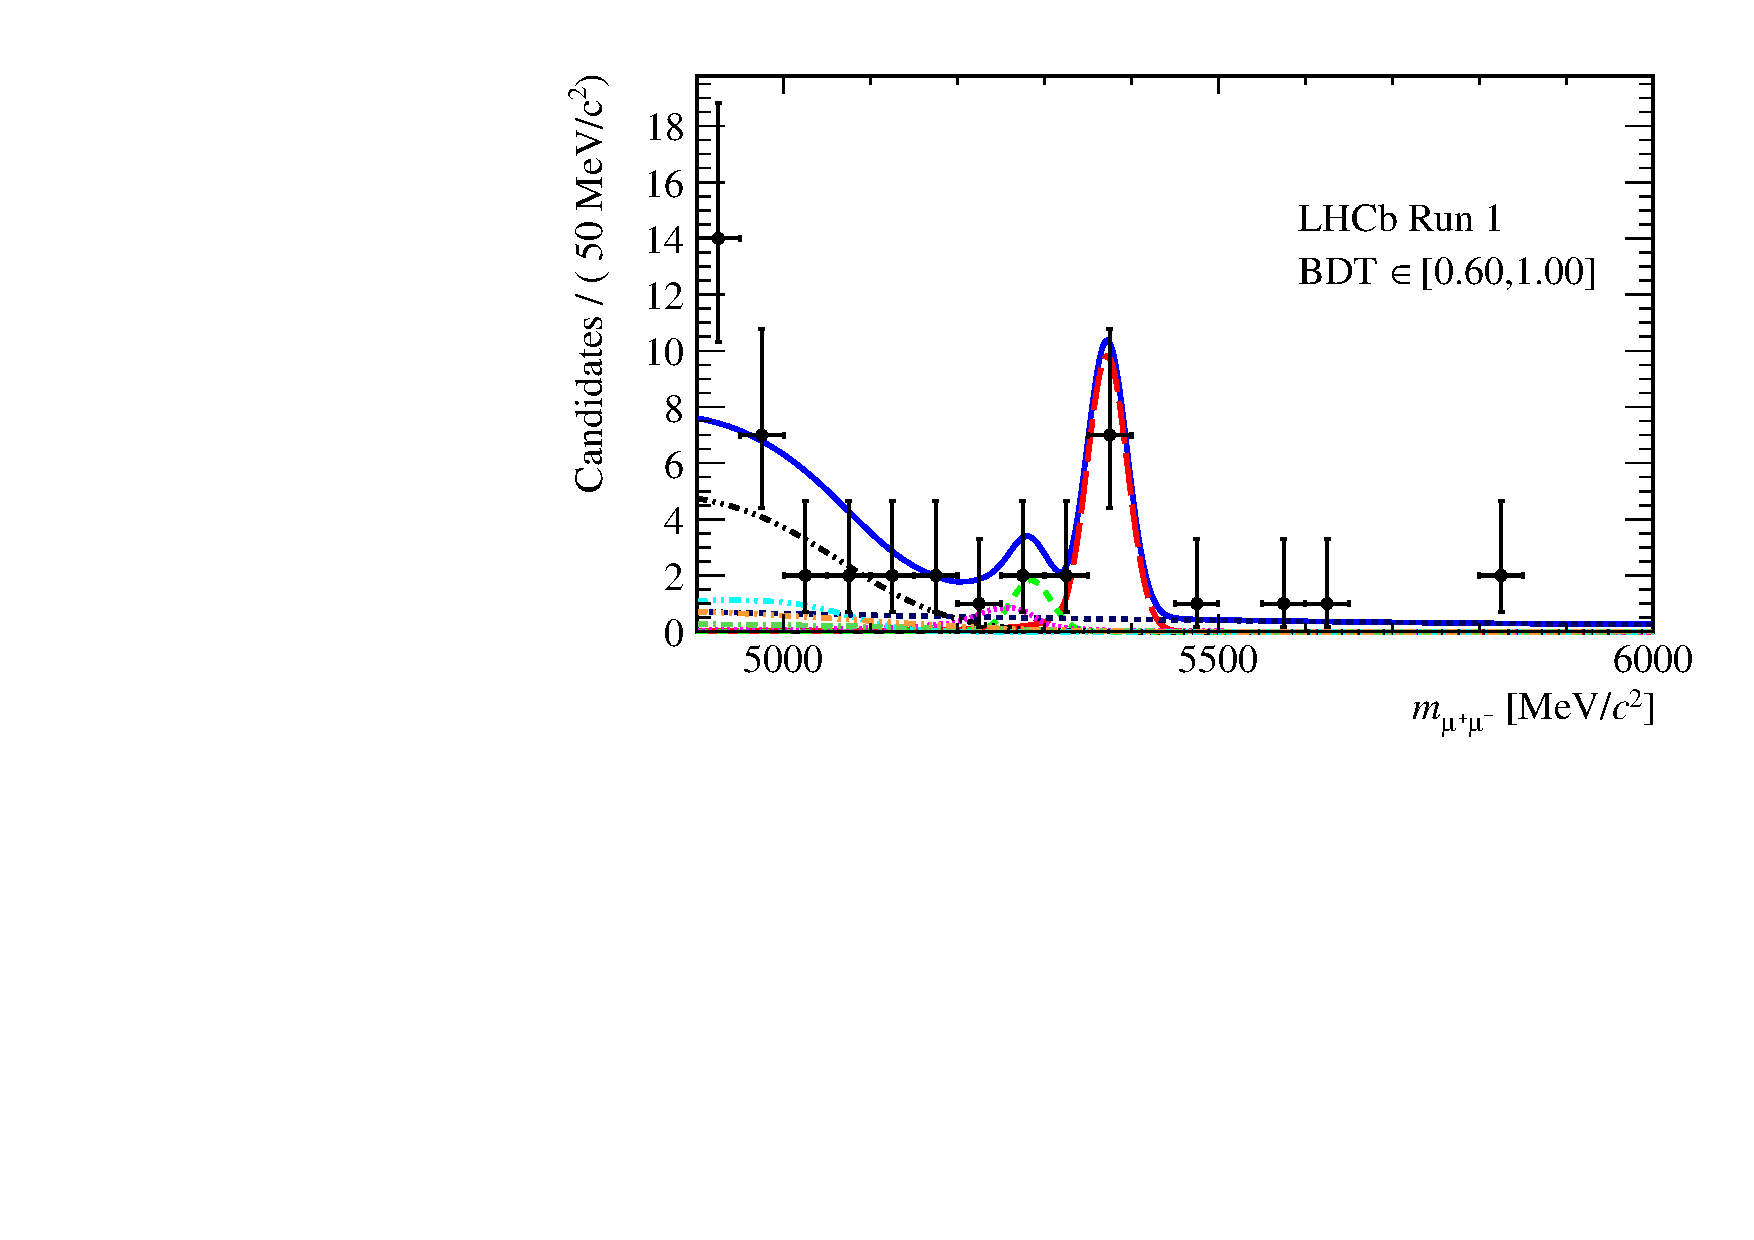
\includegraphics[width=\textwidth]{./Figs/BFAnalysis/Fig17d.pdf}
    \end{subfigure}
    ~ %add desired spacing between images, e. g. ~, \quad, \qquad, \hfill etc.                                       
      %(or a blank line to force the subfigure onto a new line)                                                      
    \begin{subfigure}[b]{0.48\textwidth}
       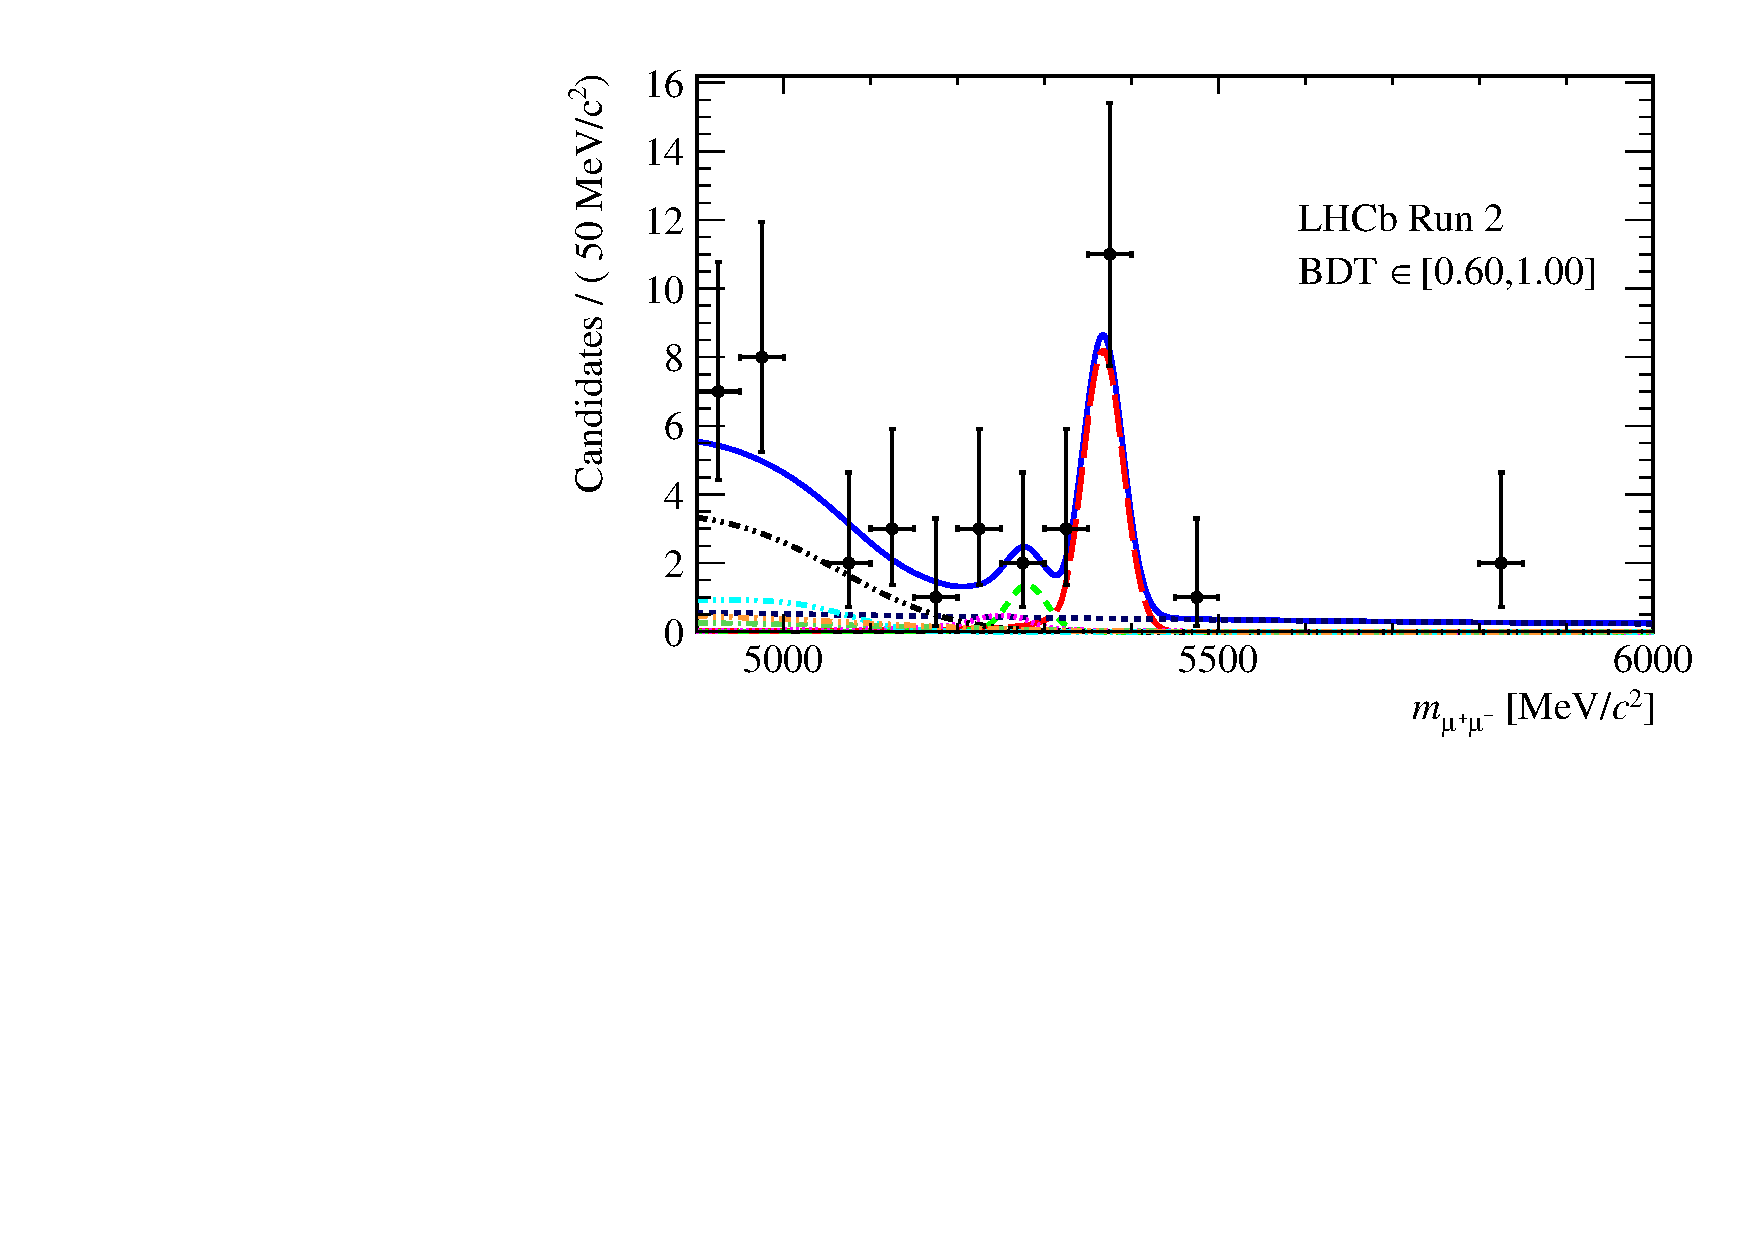
\includegraphics[width=\textwidth]{./Figs/BFAnalysis/Fig17h.pdf}
    \end{subfigure}

    \begin{subfigure}[b]{0.3\textwidth}
       \includegraphics[width=\textwidth]{./Figs/BFAnalysis/legendA.pdf}
    \end{subfigure}
    ~
    \begin{subfigure}[b]{0.3\textwidth}
       \includegraphics[width=\textwidth]{./Figs/BFAnalysis/legendB.pdf}
    \end{subfigure}
    \caption{Mass distribution in BDT bins for selected \bsmumu and \bdmumu candidates with the fit overlaid for Run\
 1 and Run 2 data. The fit includes components for \bdmumu, \bsmumu, combinatorial backgrounds and backgrounds from mis-identified decays. }
    \label{fig:BFfit}
\end{figure}



In the mass fit all \pdfs, except the combinatorial background, are constrained within Gaussian limits of their expected values based on the uncertainties \pdf parameters. 
The fraction of \bmumu decays in each BDT bin is constrained using the BDT \pdf and the yields of the mis-identified background are constrained around their expected values. The combinatorial background yields are left free in the fit and the slope of the mass distribution is required to have the same value across all bins for each data set.
%Prehaps the preceeding part about the mass fit and constraints is not needed here but could be put in the analysis strategy part more clearly?
%The fit is shown in Figure~\ref{fig:BFfit}  and the measured \BFs are
The measured \BFs are
\begin{equation}
%\begin{align}
\begin{split}
  \mathcal{B}(B^{0}_{s} \to \mu^{+} \mu^{-}) &= (3.0 \pm 0.6^{+0.3}_{-0.2}) \times 10^{-9} \\
  \mathcal{B}(B^{0} \to \mu^{+} \mu^{-}) &= (1.5^{+1.2 +0.2}_{-1.0 -0.1})    \times 10^{-10} 
%\end{align}
\end{split}
\label{eq:BFresults}
\end{equation}
where the first quoted uncertainty is the statistical uncertainty and the second is the systematic uncertainty. The dominant contributions to the systematic uncertainties are from the ratio $f_s / f_d$ and the uncertainty on the background yields for the \bsmumu and \bdmumu \BFs, respectively. %Figure~\ref{} showns the comparison of the measured \BFs and the SM predictions and Figure~\ref{fig:BFfit} shows the fit results for \bmumu candidates in the four BDT bins for both Run 1 and Run 2 data. % and Figure~\ref{fig:contour} the 2-dimensional likelihood profile for the \bdmumu and \bsmumu branching fraction measurements.
The statistical significance of the \bsmumu signal is 7.8$\sigma$ making this measurement the first single experiment observation of the \bsmumu decay. The significance of the \bdmumu signal is 1.6$\sigma$, therefore the CL$_{\text{s}}$ method~\cite{0954-3899-28-10-313} is used to place an upper limit on the branching fraction of $\mathcal{B}$(\bdmumu)$ < 3.4 \times 10^{-10}$ at the 95$\%$ confidence level.

The \bsmumu branching fraction in Equation~\ref{eq:BFresults} assumes the Standard Model value for \ADG of \ADG~=~+1, applying the corrections detailed in Section~\ref{sec:ADGBDTcorrections}; \ADG values of~0 and~$-$1 shift the central value of $\mathcal{B}$(\bsmumu) by 4.6$\%$ and 10.9$\%$, respectively. All results are consistent with the predictions of the SM as illustrated in Figure~\ref{fig:contour}.
%Figure~\ref{fig:BFfit} shows the fit results for \bmumu candidates in the four BDT bins for both Run 1 and Run 2 data.


%\begin{figure}[htbp] %Put in the summary.
%    \centering
%        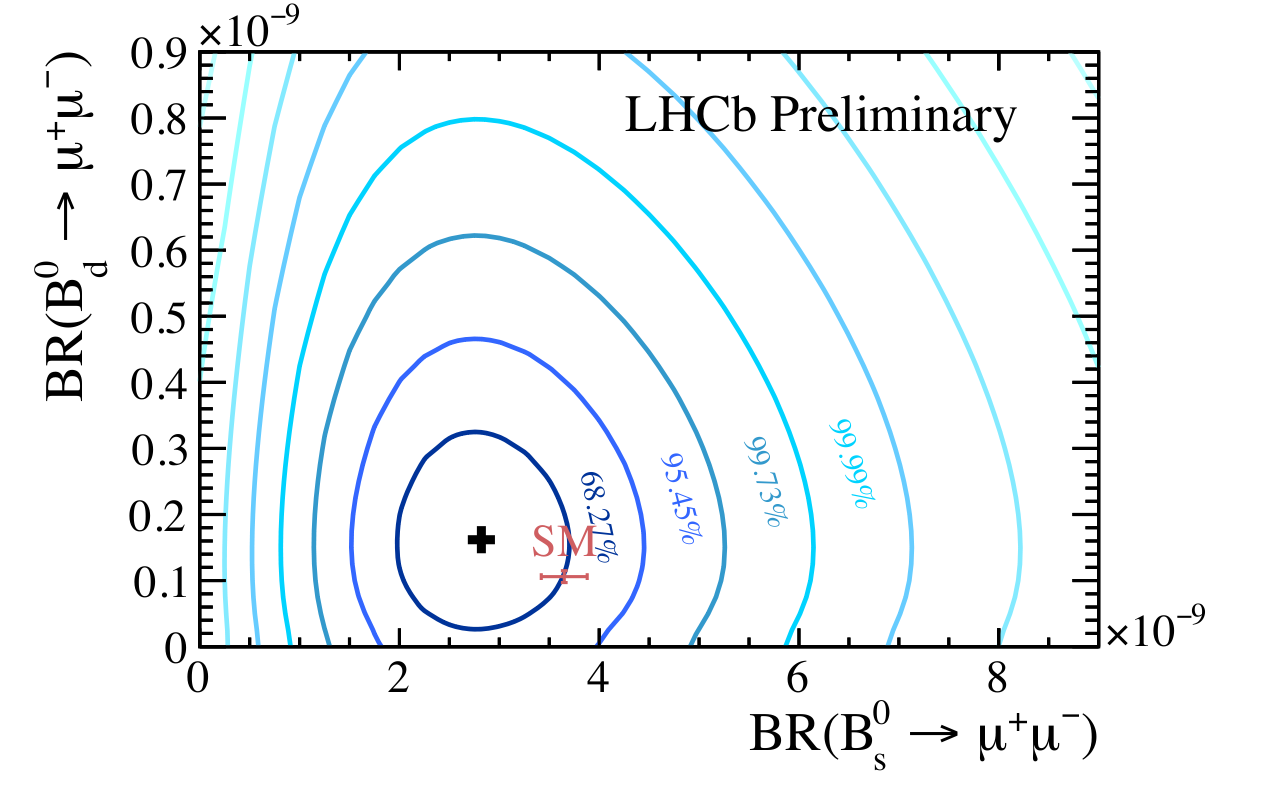
\includegraphics[width= 0.6 \textwidth]{./Figs/BFAnalysis/2D_contour_plot.png}
%      \caption{\bdmumu and \bsmumu 2-dimesnional likelihood plot for the simultaneous branching fraction fit to Run 1 and Run 2 data. }
%    \label{fig:contour}
%\end{figure}


%\begin{figure}[tbp]
%    \centering
%    \begin{subfigure}[b]{0.48\textwidth}
%        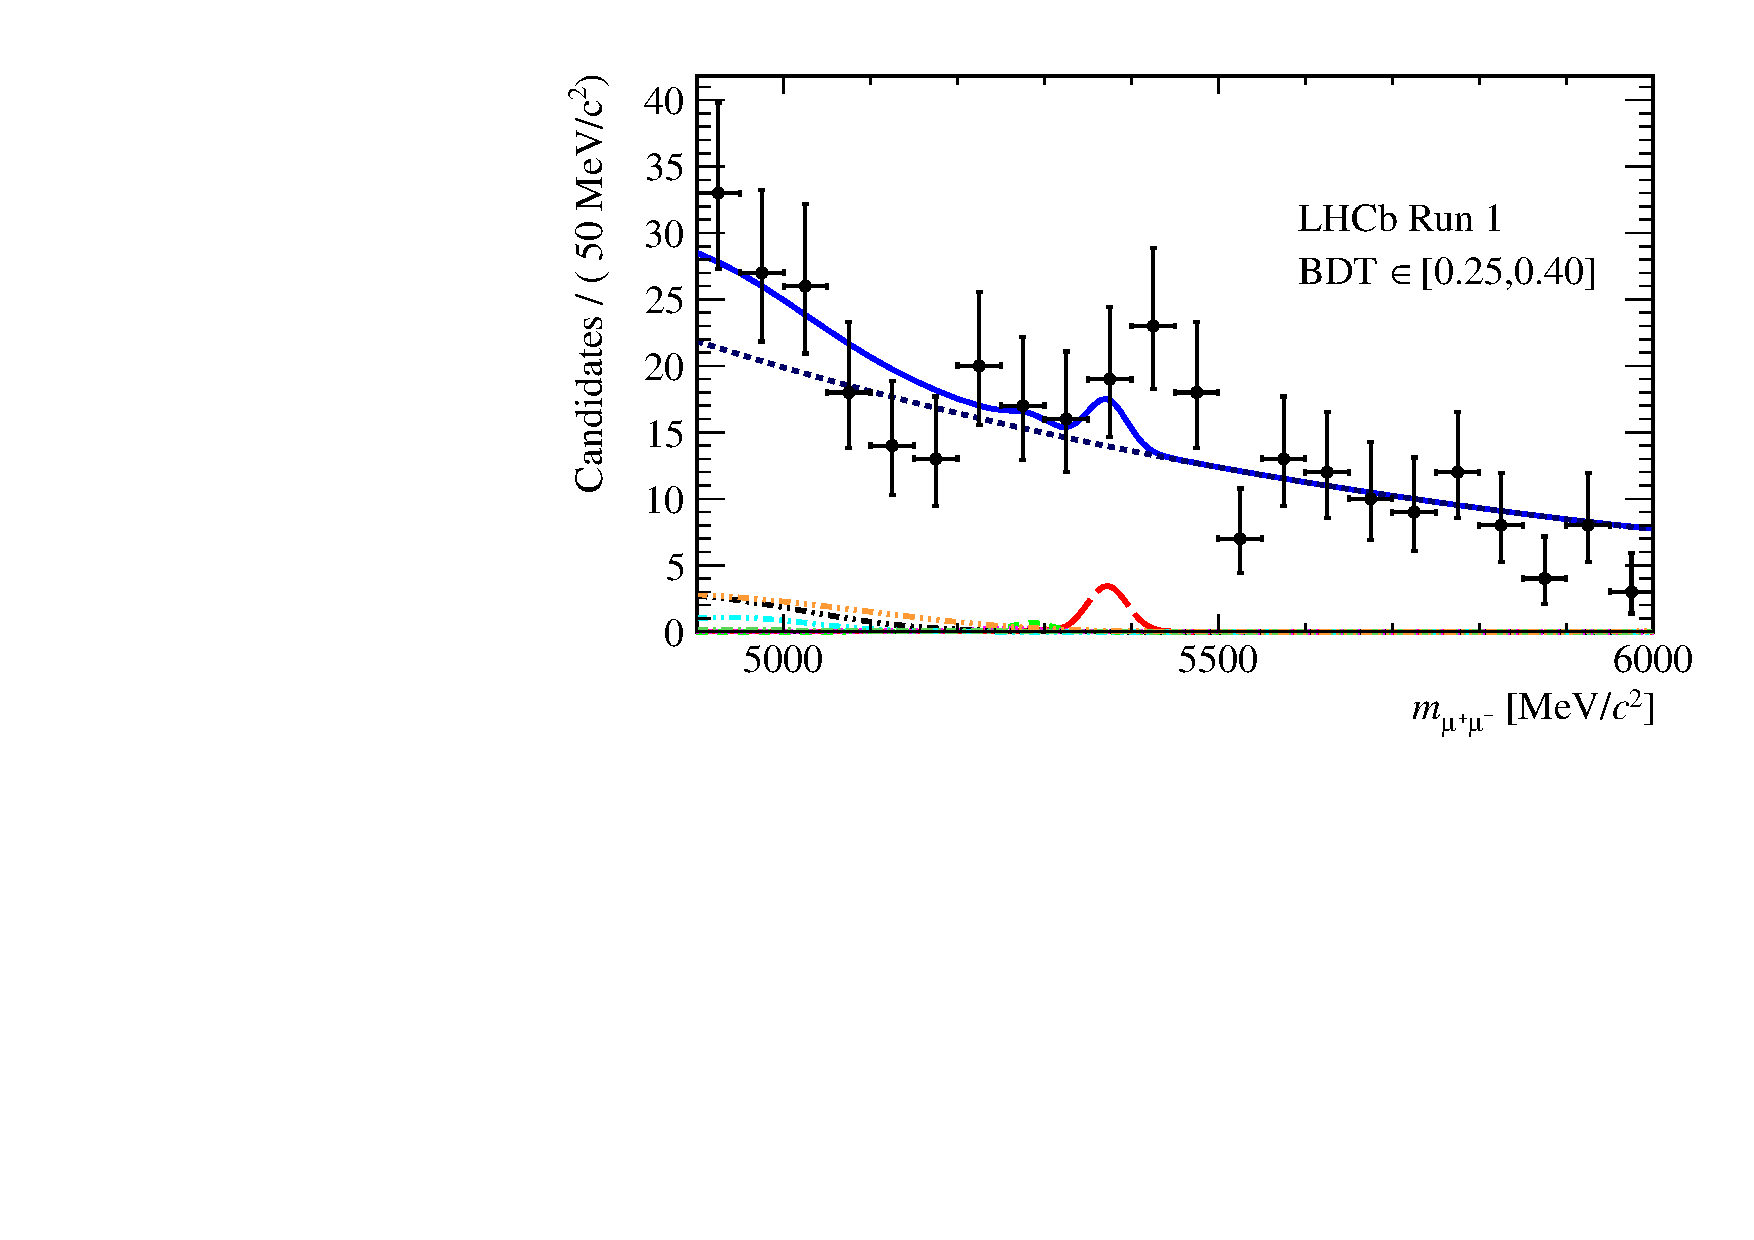
\includegraphics[width=\textwidth]{./Figs/BFAnalysis/Fig17a.pdf}
%    \end{subfigure}
%    ~ %add desired spacing between images, e. g. ~, \quad, \qquad, \hfill etc. 
%      %(or a blank line to force the subfigure onto a new line)
%    \begin{subfigure}[b]{0.48\textwidth}
%       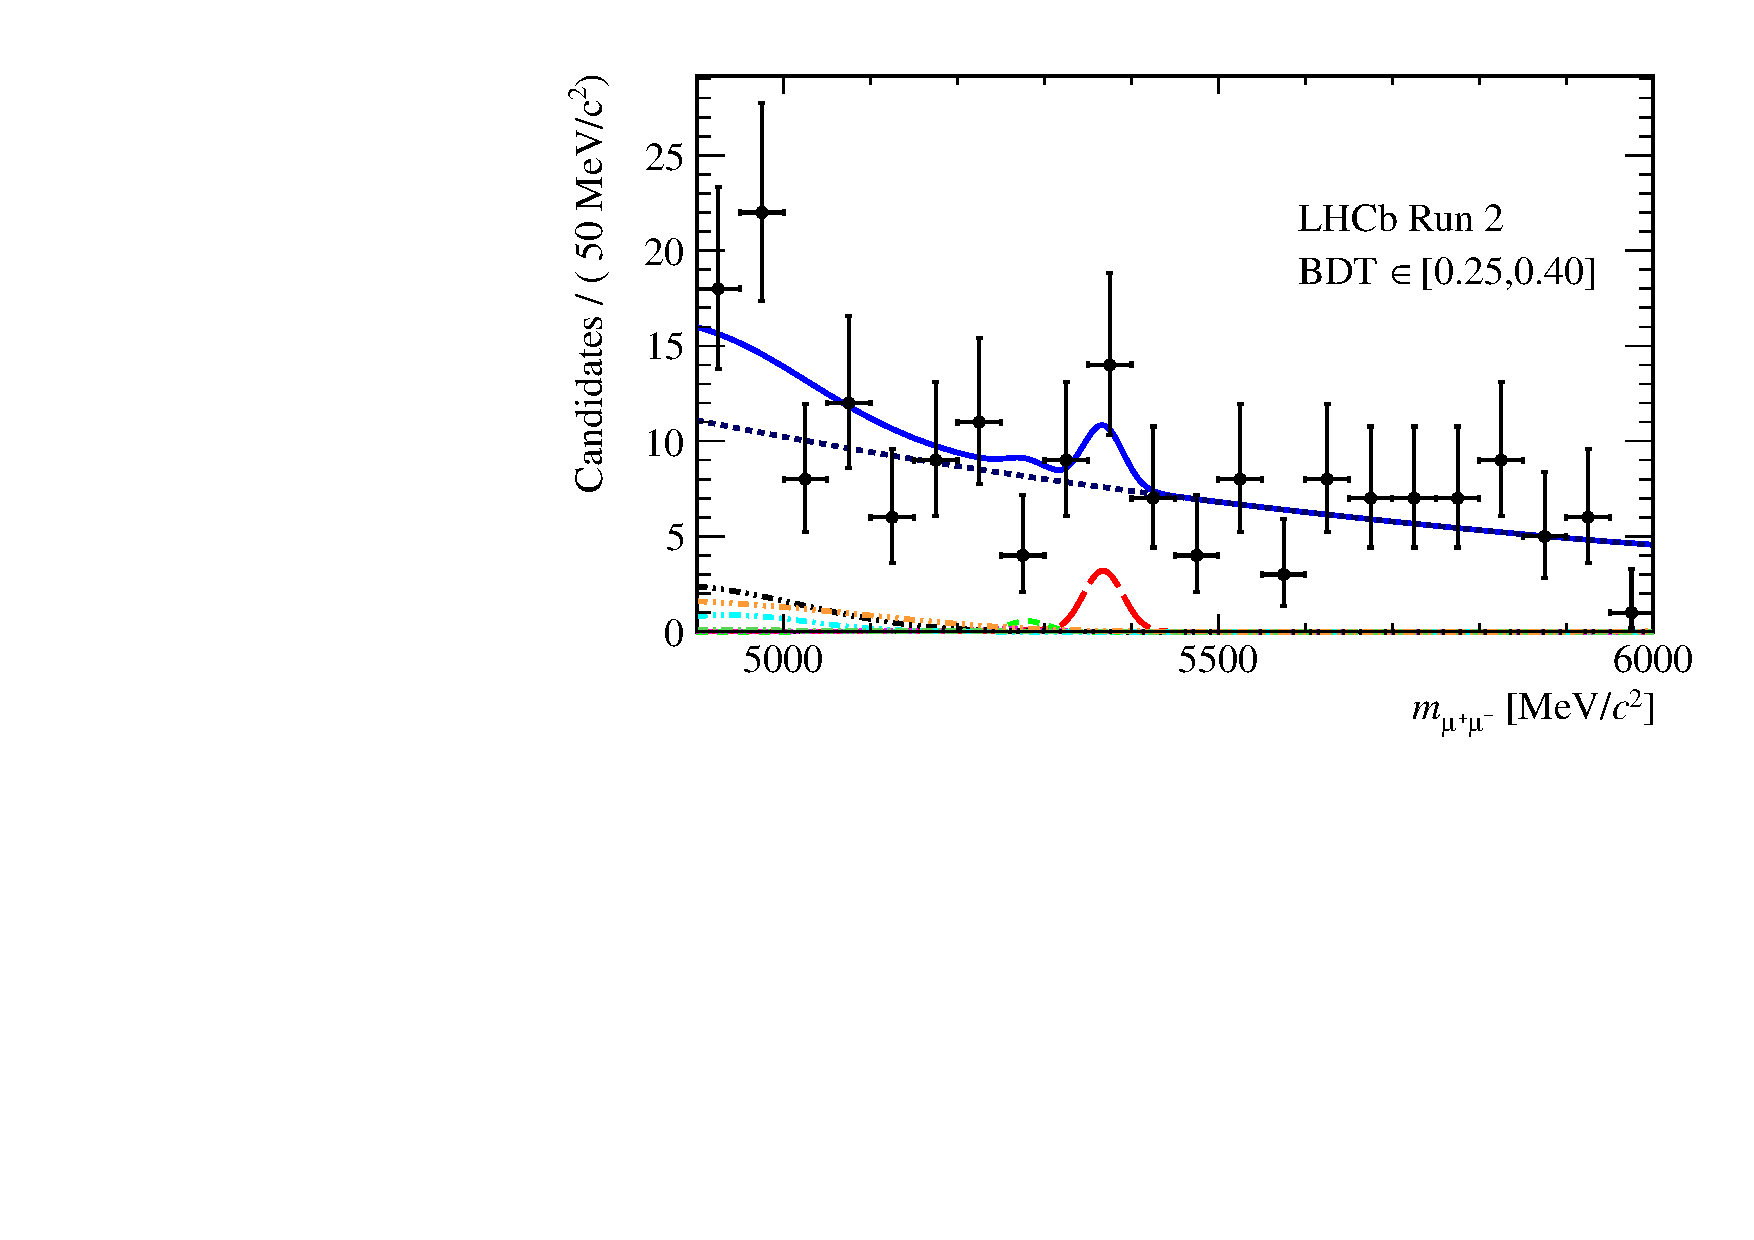
\includegraphics[width=\textwidth]{./Figs/BFAnalysis/Fig17e.pdf}
%    \end{subfigure}
%    \begin{subfigure}[b]{0.48\textwidth}
%        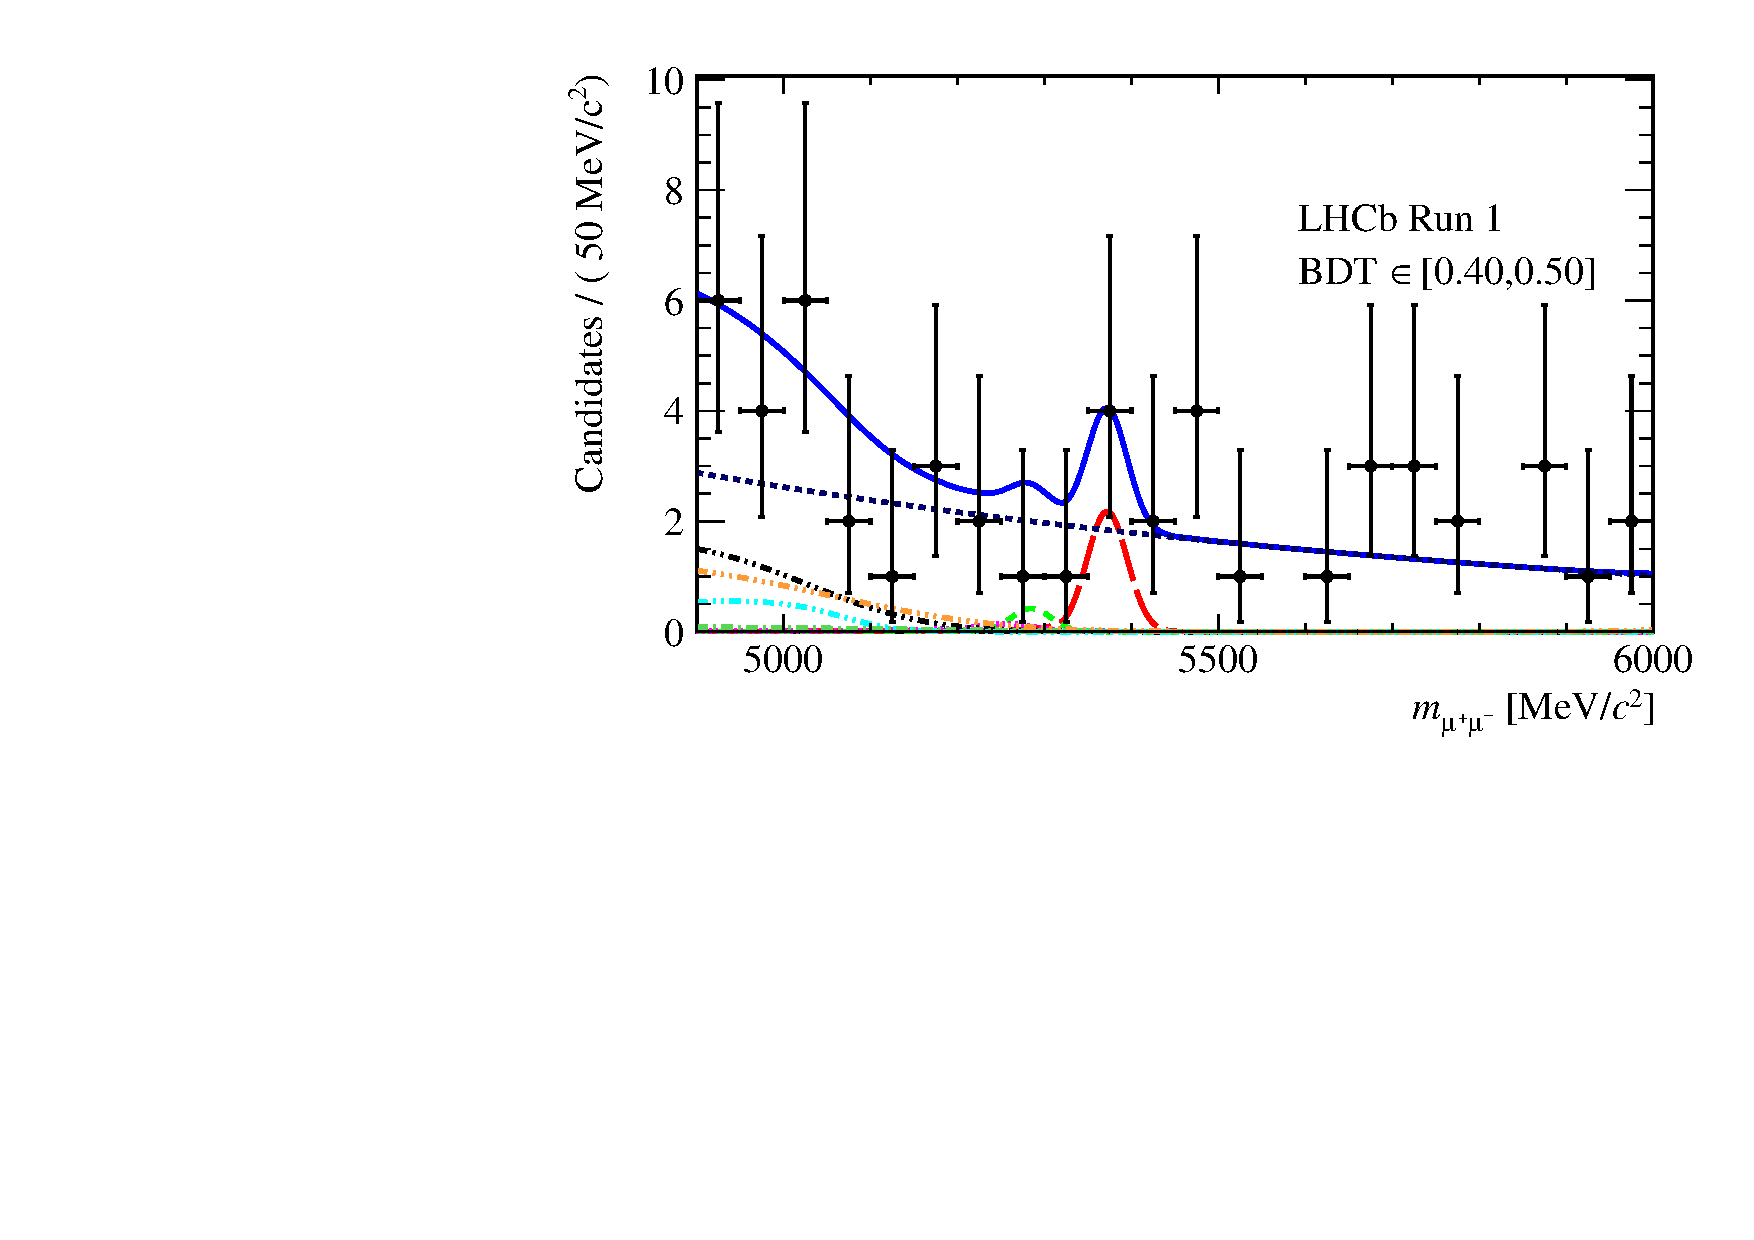
\includegraphics[width=\textwidth]{./Figs/BFAnalysis/Fig17b.pdf}
%    \end{subfigure}
%    ~ %add desired spacing between images, e. g. ~, \quad, \qquad, \hfill etc. 
%      %(or a blank line to force the subfigure onto a new line)
%    \begin{subfigure}[b]{0.48\textwidth}
%       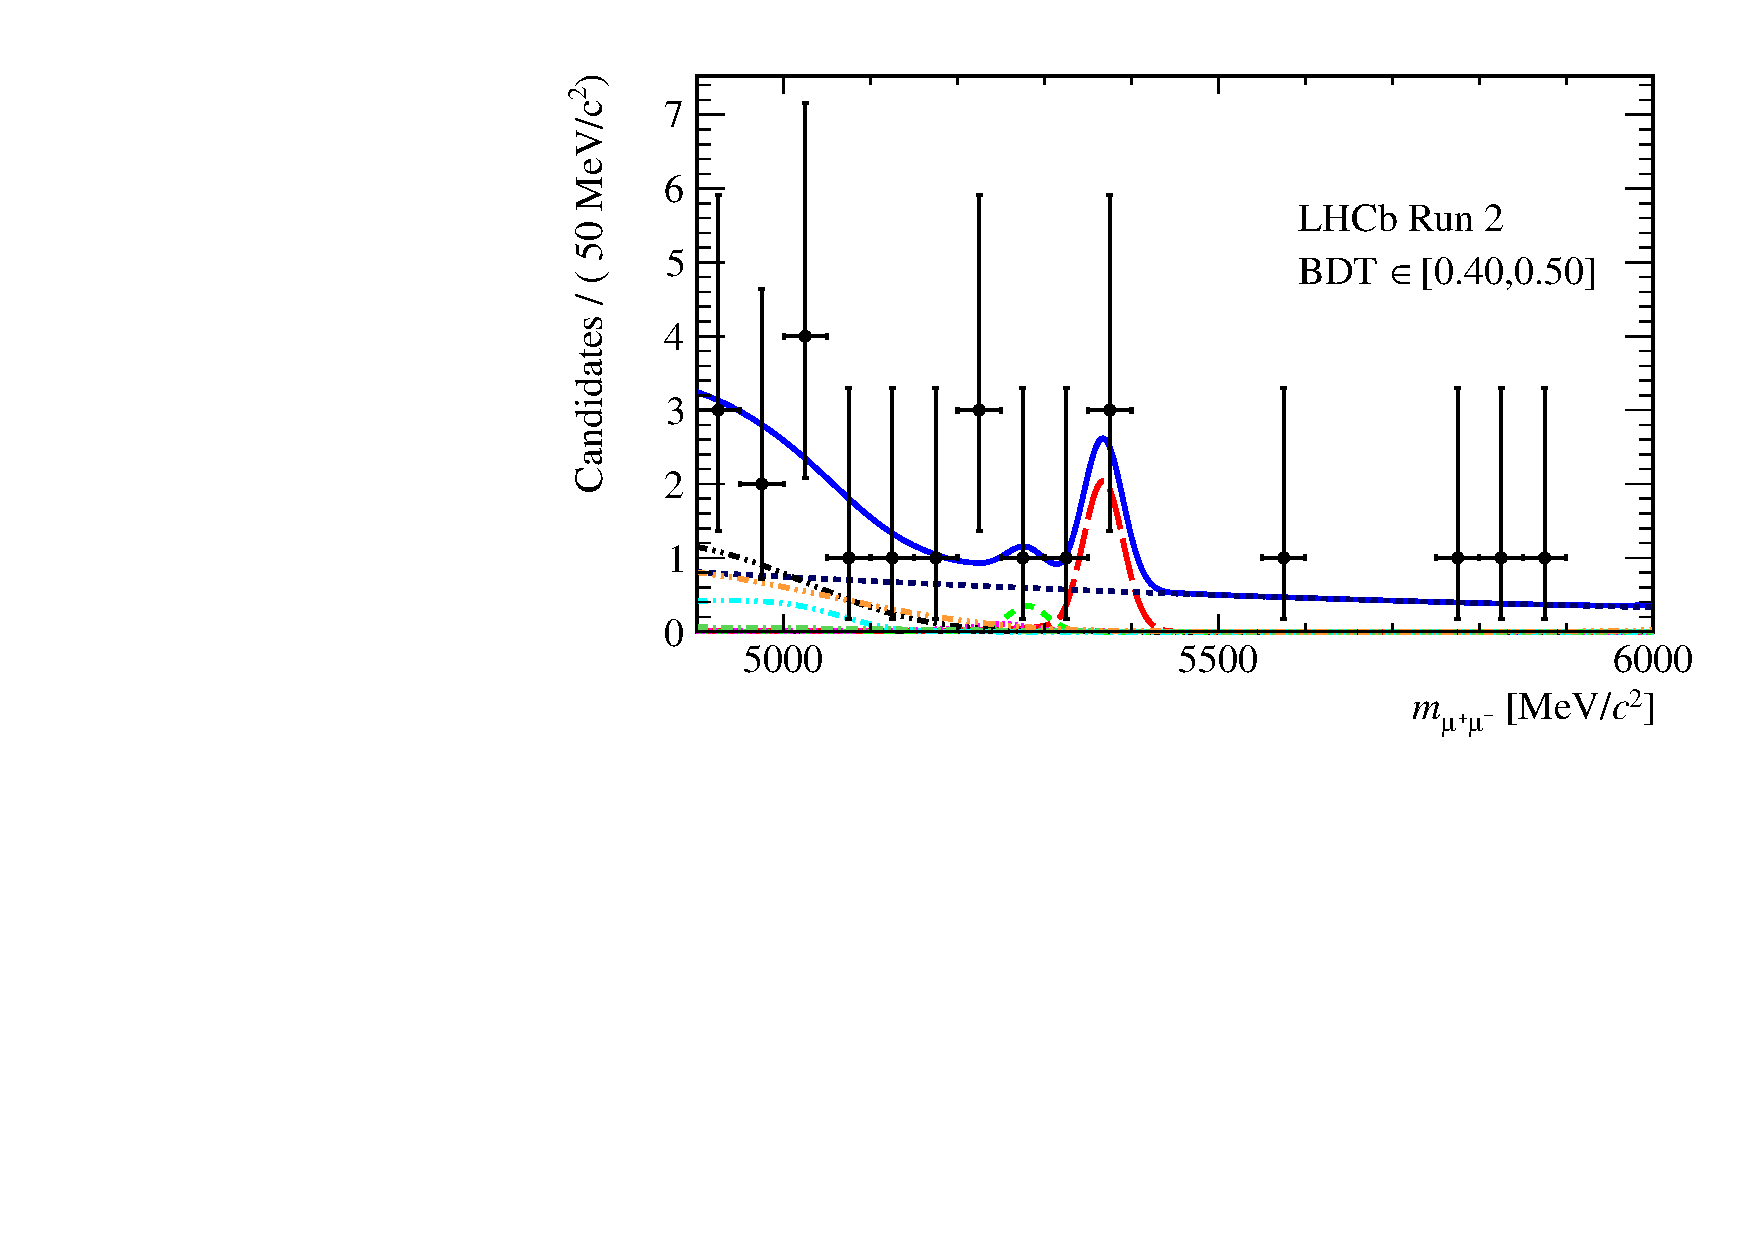
\includegraphics[width=\textwidth]{./Figs/BFAnalysis/Fig17f.pdf}
%    \end{subfigure}
%    ~
%      \begin{subfigure}[b]{0.48\textwidth}
%        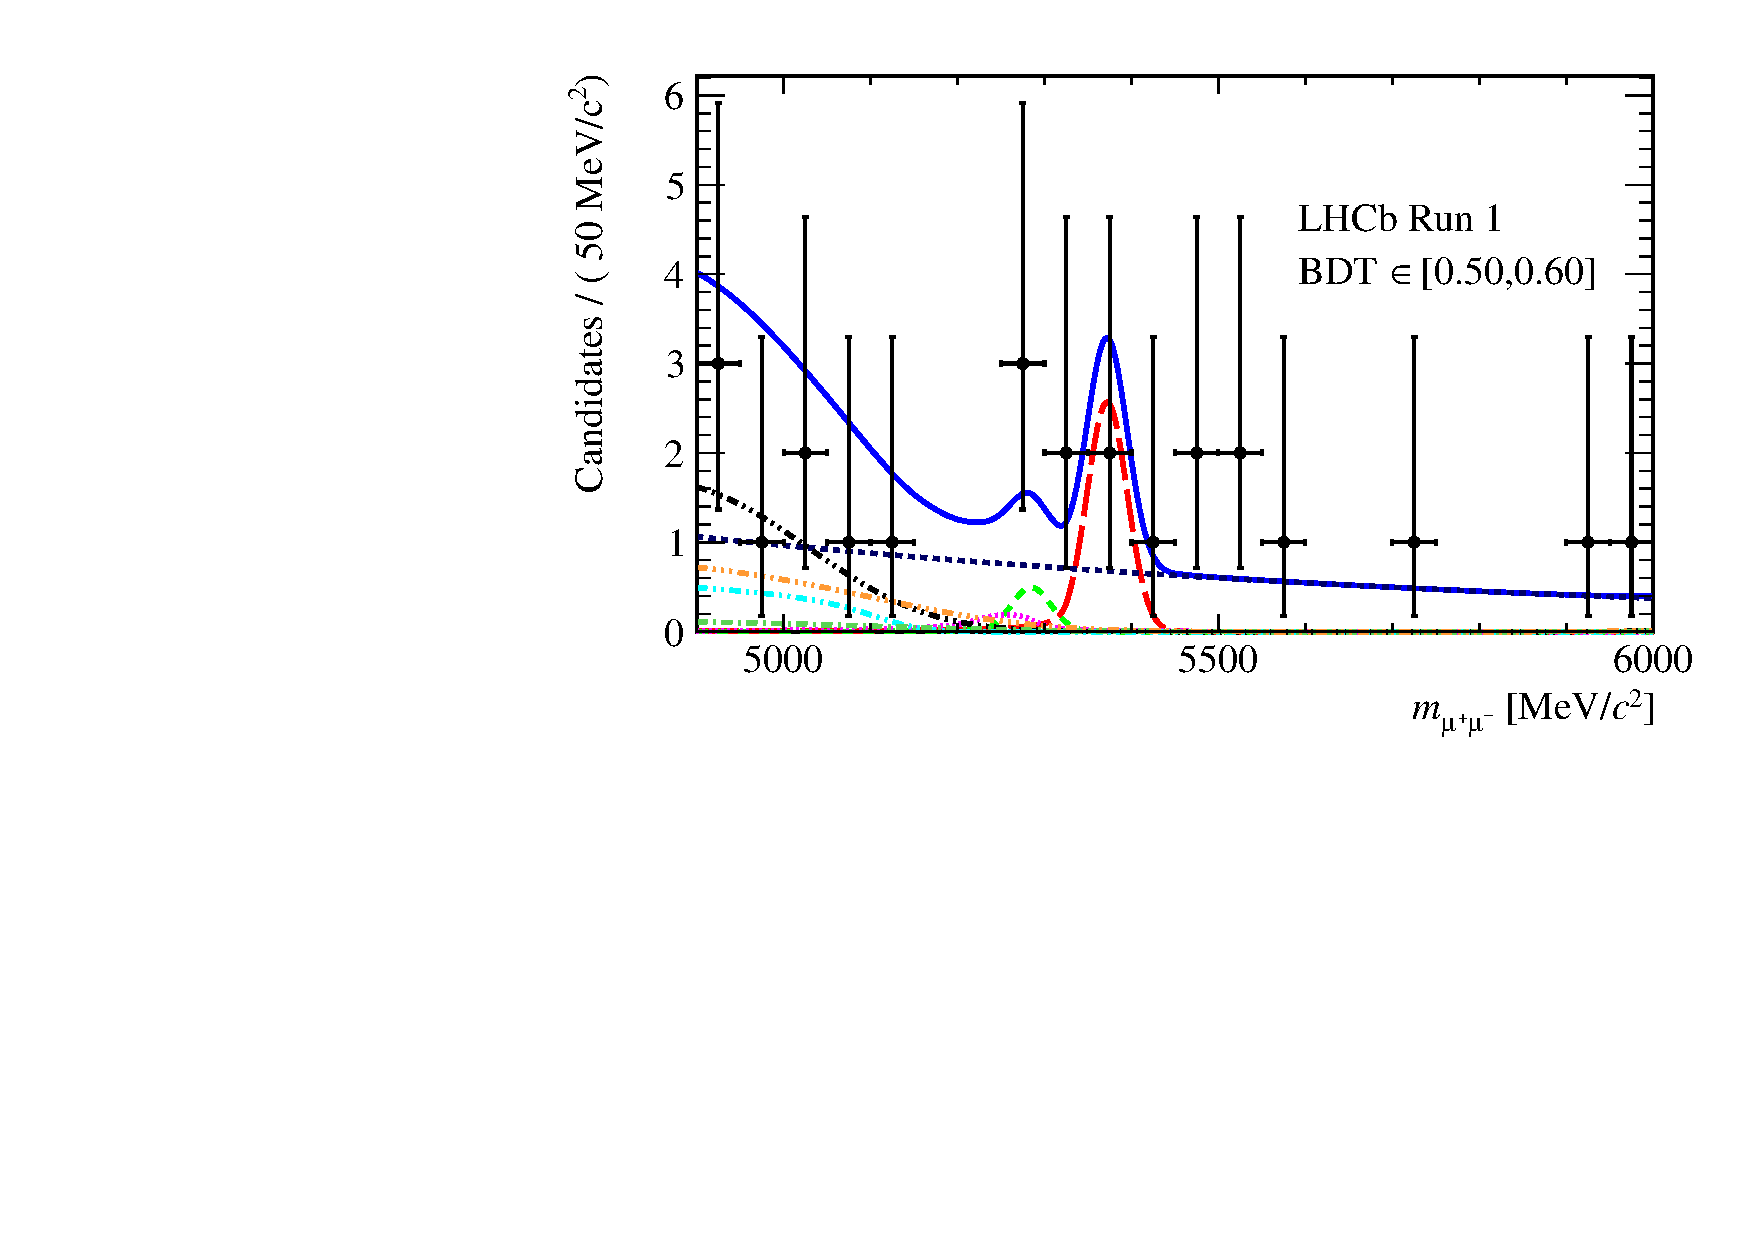
\includegraphics[width=\textwidth]{./Figs/BFAnalysis/Fig17c.pdf}
%    \end{subfigure}
%    ~ %add desired spacing between images, e. g. ~, \quad, \qquad, \hfill etc. 
%      %(or a blank line to force the subfigure onto a new line)
%    \begin{subfigure}[b]{0.48\textwidth}
%       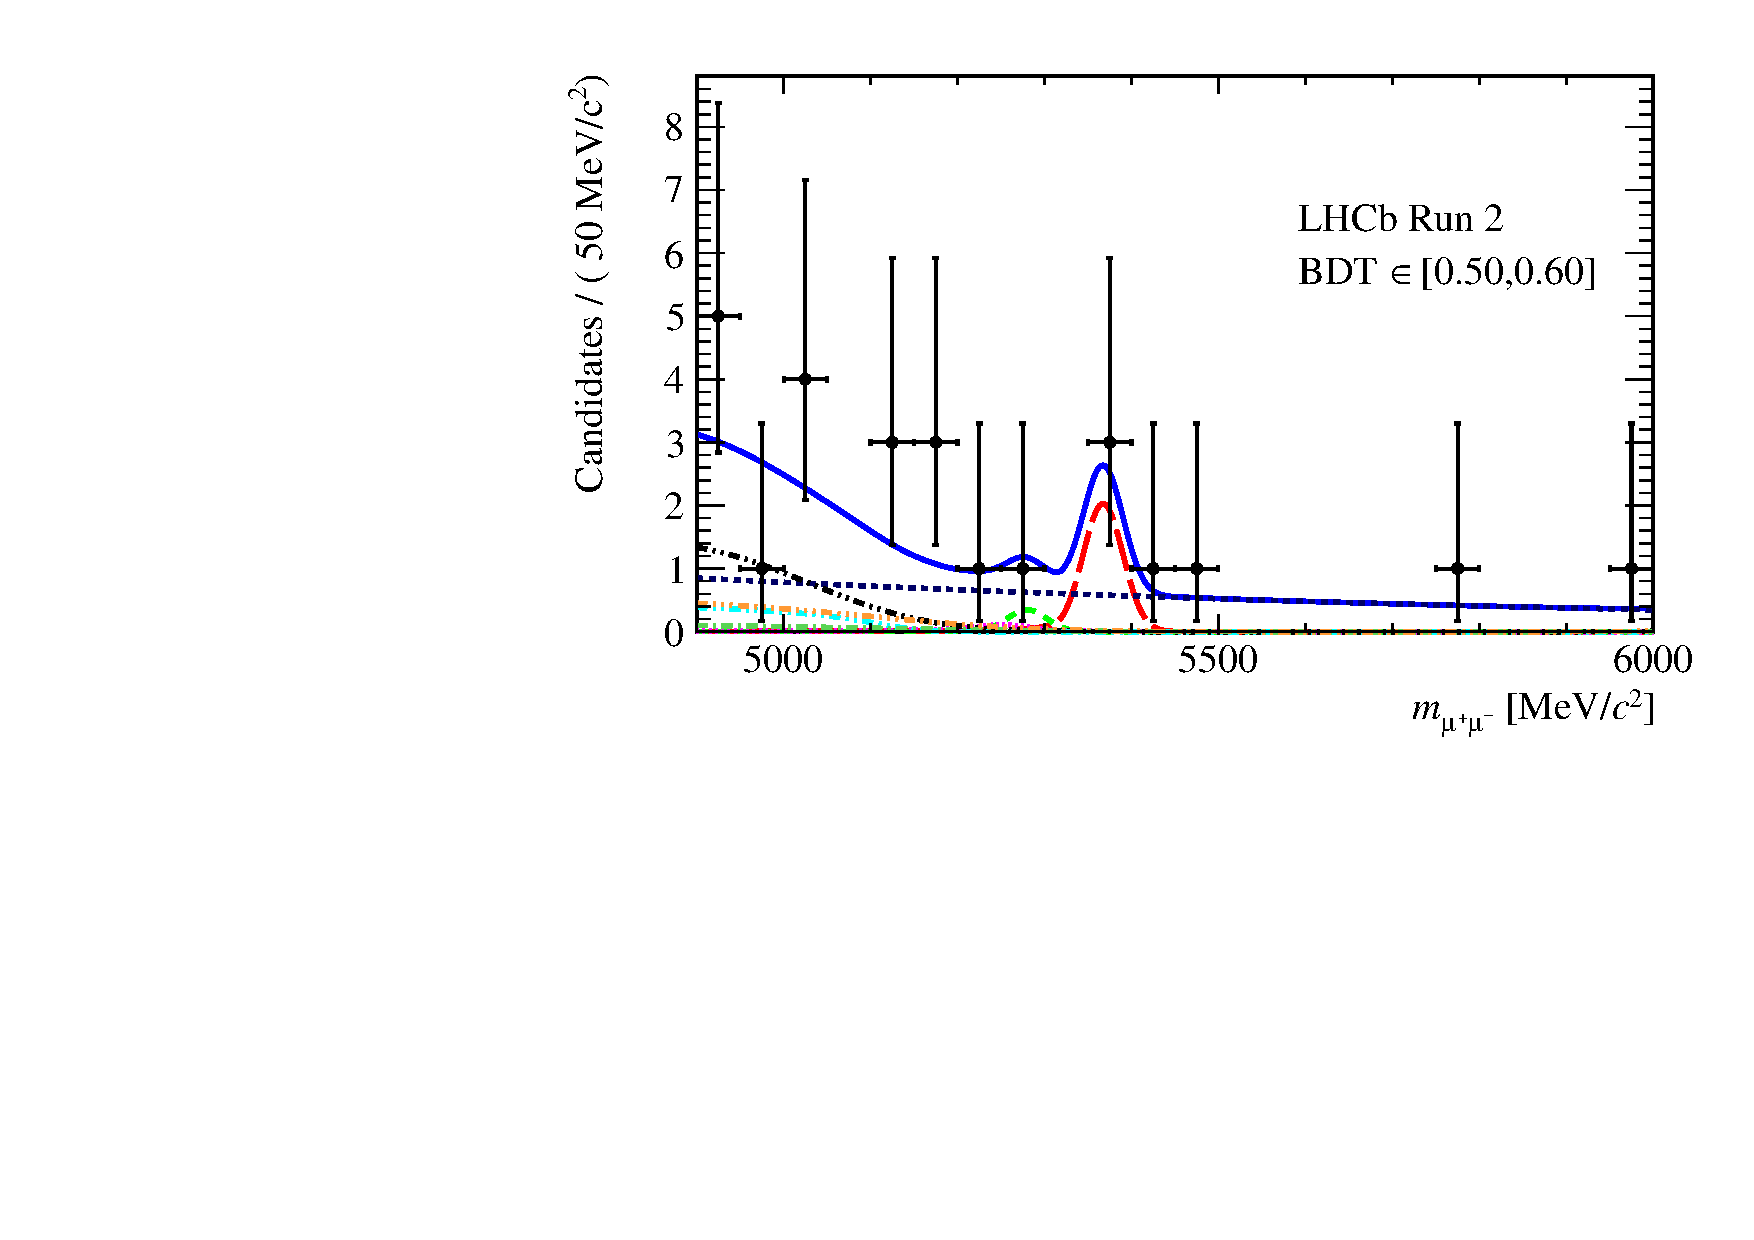
\includegraphics[width=\textwidth]{./Figs/BFAnalysis/Fig17g.pdf}
%    \end{subfigure}
%    \begin{subfigure}[b]{0.48\textwidth}
%        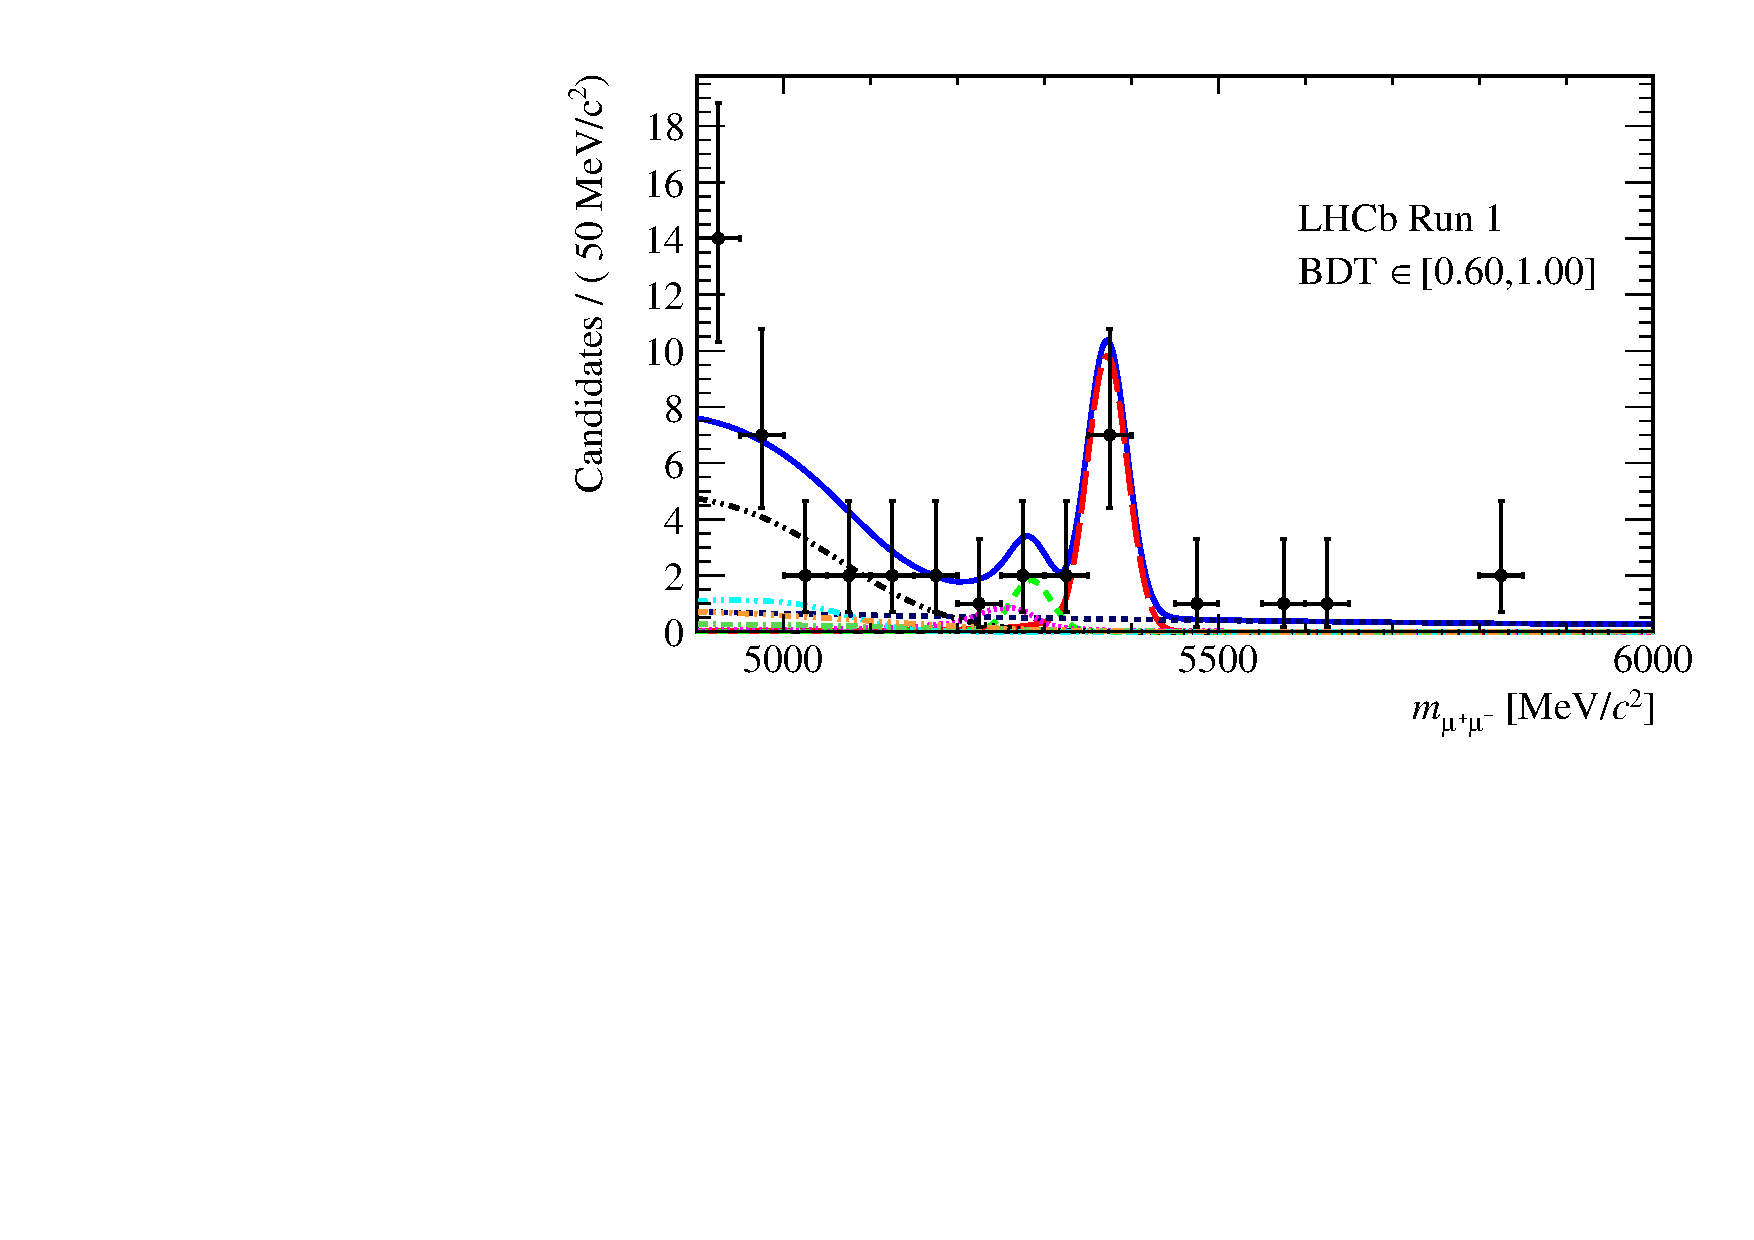
\includegraphics[width=\textwidth]{./Figs/BFAnalysis/Fig17d.pdf}
%    \end{subfigure}
%    ~ %add desired spacing between images, e. g. ~, \quad, \qquad, \hfill etc. 
%      %(or a blank line to force the subfigure onto a new line)
%    \begin{subfigure}[b]{0.48\textwidth}
%       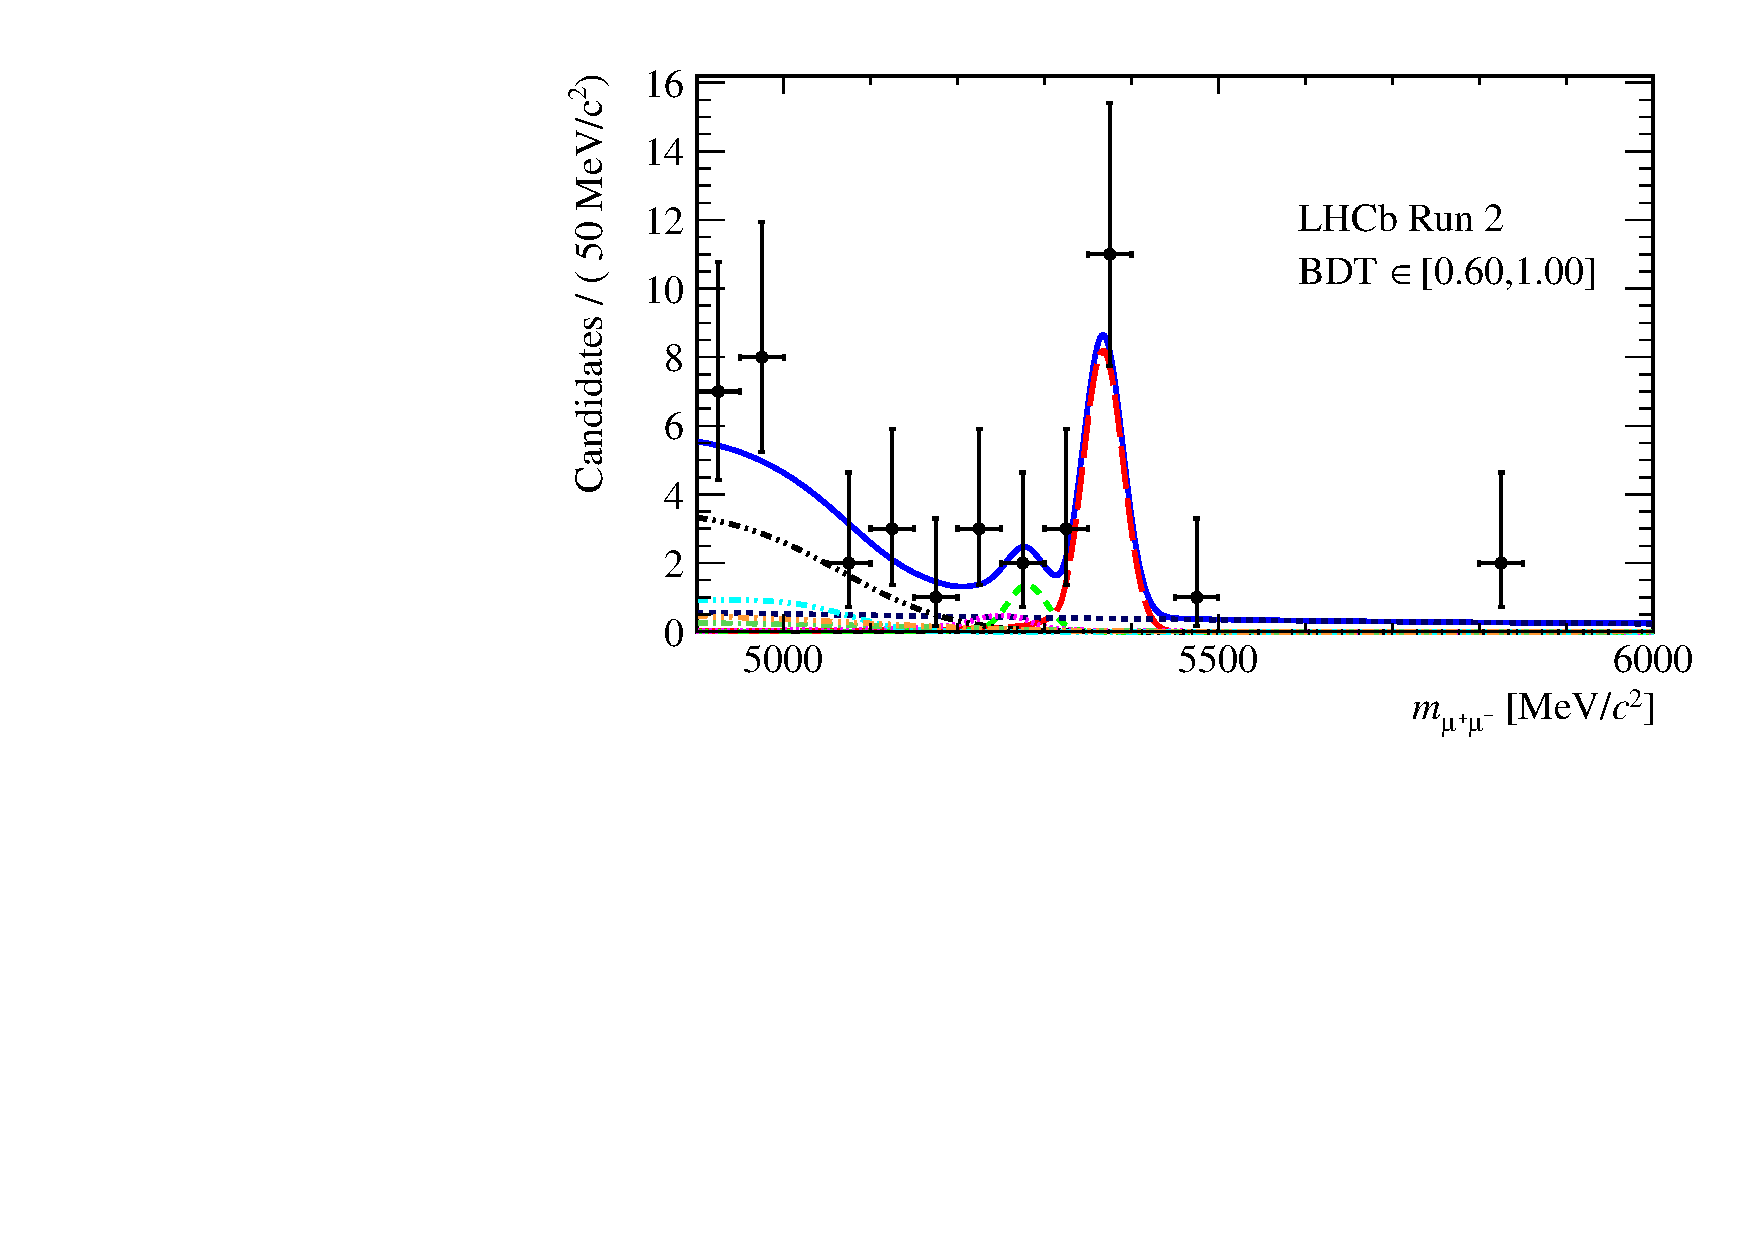
\includegraphics[width=\textwidth]{./Figs/BFAnalysis/Fig17h.pdf}
%    \end{subfigure}%

%    \begin{subfigure}[b]{0.3\textwidth}
%       \includegraphics[width=\textwidth]{./Figs/BFAnalysis/legendA.pdf}
%    \end{subfigure}
%    ~
%    \begin{subfigure}[b]{0.3\textwidth}
%       \includegraphics[width=\textwidth]{./Figs/BFAnalysis/legendB.pdf}
%    \end{subfigure}
%    \caption{Mass distribution in BDT bins for selected \bsmumu and \bdmumu candidates with the fit overlaid for Run 1 and Run 2 data. The fit includes components for \bdmumu, \bsmumu, combinatorial backgrounds, mis-identified \bhh decays and backgrounds from semi-leptonic decays. }
%    \label{fig:BFfit}
%\end{figure}



%{\bf some things I should learn about the BF analysis or I think I should mention. The correlation, orlack ok, between the mass and BDT output. The cascade B decays that are removed by the lower 4900 mass cut (Alessio) and also the decays that contribute to CBG (Siim).}

%{\it prehaps put plots and numbers in the appendix??}

\begin{figure}[htbp] %Put in the summary.                                                                                
      \centering
        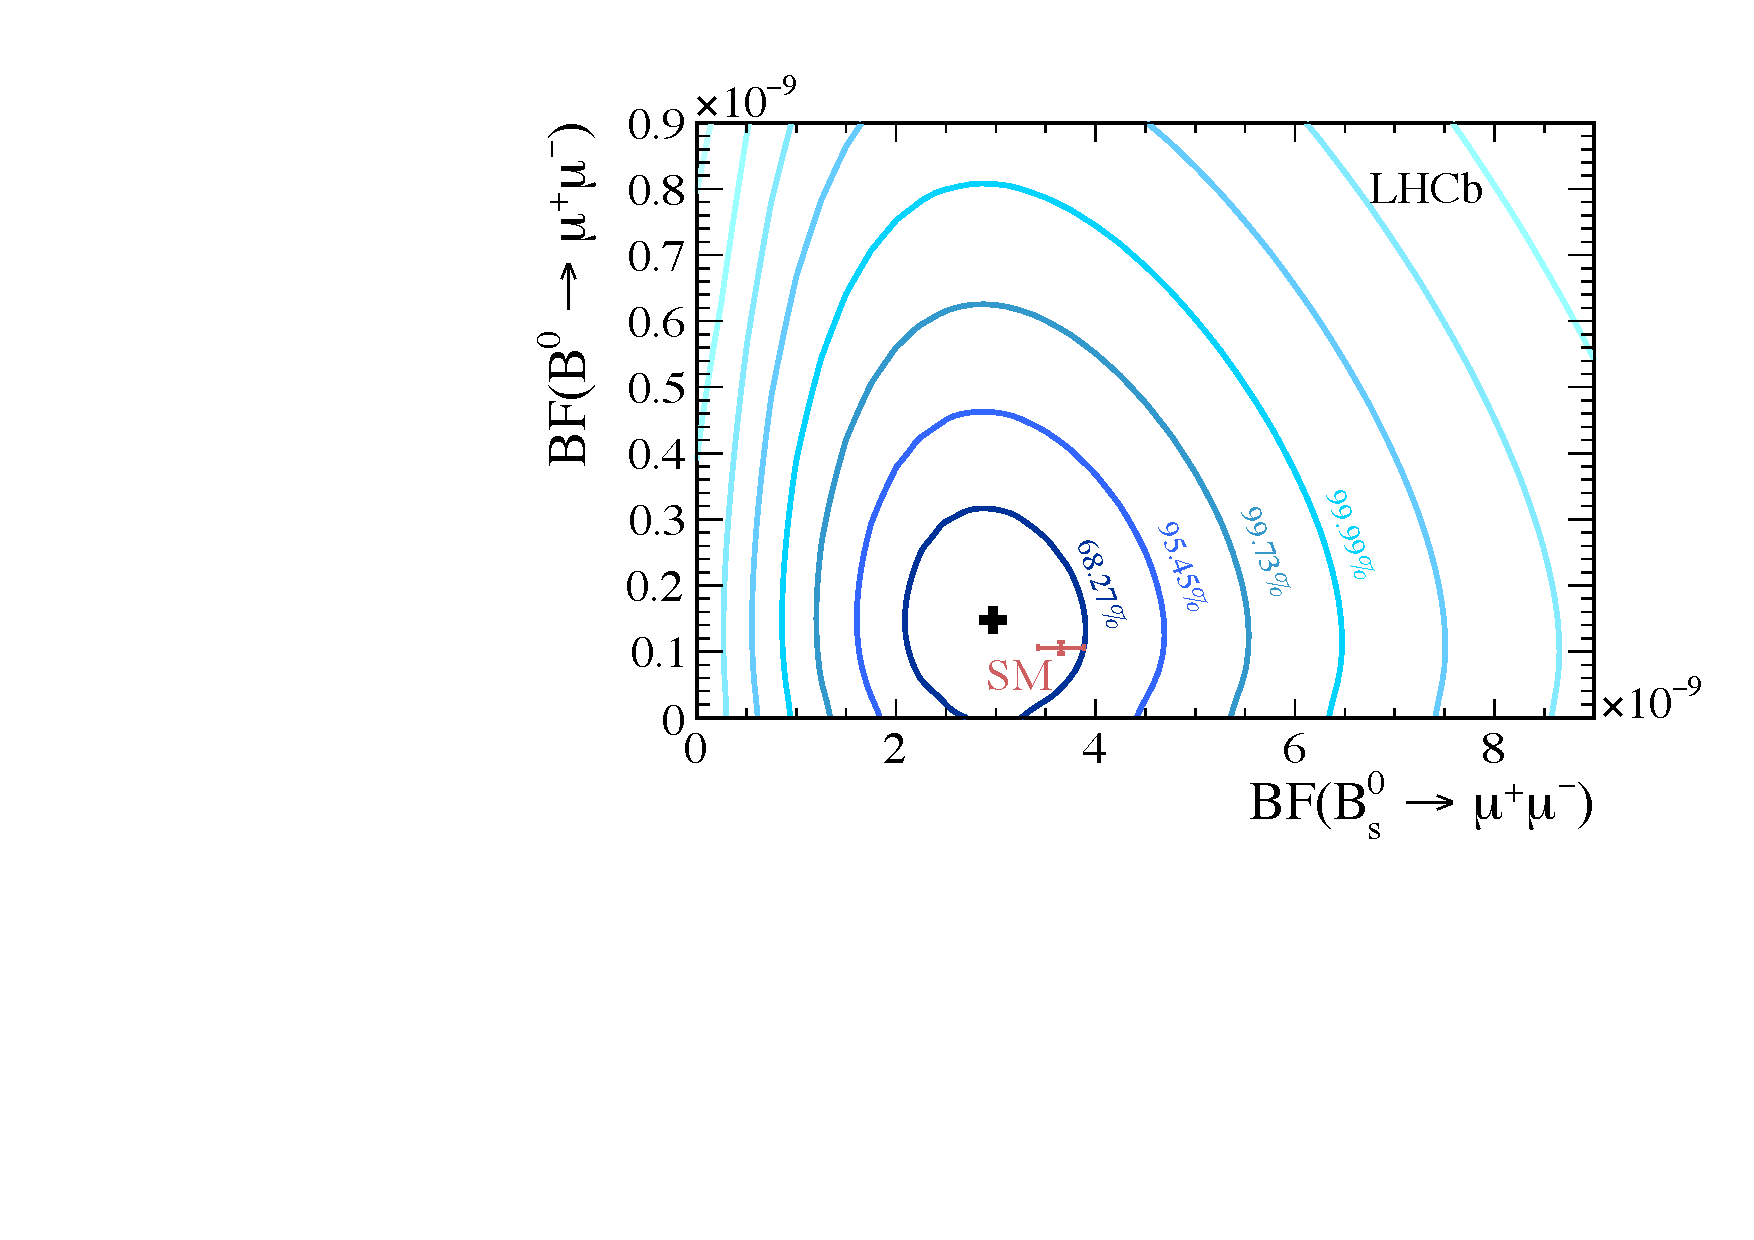
\includegraphics[width= 0.8 \textwidth]{./Figs/BFAnalysis/2D_contour_plot.pdf}
      \caption{\bdmumu and \bsmumu 2-dimensional likelihood plot for the simultaneous branching fraction fit to Run 1 and Run 2 data. }
    \label{fig:contour}
\end{figure}

